%% Phd thesis of Niklas Michel
%% ===========================
%% based on the template of Phd thesis of Jonas Gunst
%%
%% You need at least KomaScript v3.0.0,
%% e.g. available in Texlive 2009

\documentclass  [
  paper           = a4,
  BCOR            = 13mm, %8.25mm bis 18mm
  twoside,
  fontsize        = 11pt, %12
  DIV             = 12,   %oder: 10 bzw. 13 bzw. 14
  %fleqn,
  %bibtotoc,
  %liststotoc,
  %toc             = bibnumbered,
  %toc             = listofnumbered,
  chapterprefix,
  numbers         = noendperiod,
  headinclude     = true,
  footinclude     = false,
  headings        = big,
  headings        = openright,
  headsepline     = true,
  footsepline     = false,
  cleardoublepage = empty,
%  listof          = leveldown,
  titlepage       = true
]                                       {scrbook}

% used pagages
\usepackage     [utf8]                  {inputenc}
\usepackage     [T1]                    {fontenc}
\usepackage                             {color}
\usepackage                             {amsmath,amsfonts,amssymb}
\usepackage                             {bm,bbold}
%\usepackage                             {}
\usepackage                             {graphicx,nicefrac}
\usepackage     [english]               {babel}
%\usepackage     [numbers,sort&compress] {natbib}
\usepackage         					{hyperref}
\usepackage                             {lmodern}
%\usepackage                             {txfonts}
%\usepackage                             {multirow}
%\usepackage                             {hhline}
\usepackage{enumerate}
\usepackage[toc,page,header]{appendix}
\usepackage{cite}
\usepackage{multirow}
\usepackage{colortbl}
\usepackage{combelow}
\usepackage{scrlayer-scrpage}
\usepackage{mathtools}
\mathtoolsset{showonlyrefs=true}%show only referenced eqs.
\usepackage{cases}

\setcounter{secnumdepth}{3}
\setcounter{tocdepth}{2}

\usepackage[margin=10pt,format=plain,font=small,labelfont=bf,labelsep=colon]{caption}
%indention=0.5cm,labelsep=endash
\usepackage[caption=false]{subfig}

\captionsetup[subfigure]{textfont=small, subrefformat=simple,labelformat=simple,listofformat=subsimple}
%labelfont={normalsize,bf},
\renewcommand\thesubfigure{(\alph{subfigure})}


%
%\usepackage{bbold,tikz,bm,nicefrac,slashed}
%\usepackage{subfigure,url,booktabs,enumerate}
%\usepackage[american]{babel}
%\selectlanguage{american}
%\usepackage[automark,headsepline]{scrpage2}
%\usepackage{titlesec,cleveref}
%\usepackage[inner=30mm,outer=30mm,top=25mm,bottom=30mm,a4paper,twoside]{geometry}
%\usepackage{calc}
%\usepackage{tocloft}


% Mathcalboondox
\DeclareFontFamily{U}{BOONDOX-calo}{\skewchar\font=45 }
\DeclareFontShape{U}{BOONDOX-calo}{m}{n}{
  <-> s*[1.05] BOONDOX-r-calo}{}
\DeclareFontShape{U}{BOONDOX-calo}{b}{n}{
  <-> s*[1.05] BOONDOX-b-calo}{}
\DeclareMathAlphabet{\mathcalboondox}{U}{BOONDOX-calo}{m}{n}
\SetMathAlphabet{\mathcalboondox}{bold}{U}{BOONDOX-calo}{b}{n}
\DeclareMathAlphabet{\mathbcalboondox}{U}{BOONDOX-calo}{b}{n}

%\usepackage{mathrsfs}
%\usepackage[cal=cm,scr=boondoxo,scrscaled=1.05]{mathalfa}

 
% Colors

\definecolor{mpgcolor}{rgb}{0.00,0.494117647,0.478431373}
\definecolor{goldenrod}{rgb}{0.85490196, 0.647058823, 0.125490196}
\definecolor{gold}{rgb}{1, 0.843137254, 0.0}
\definecolor{fore}{RGB}{249,242,215}
\definecolor{back}{RGB}{51,51,51}
\definecolor{keywords}{RGB}{255,0,90}
\definecolor{comments}{RGB}{60,179,113}
\definecolor{ubuntured}{rgb}{0.7882353, 0.0, 0.0862745}
\definecolor{MYgreen}{rgb}{0.2352941, 0.7019608, 0.4431373}


% Tables

\newcolumntype{C}[1]{>{\centering\arraybackslash}p{#1}}


% Captions
%\setkomafont{caption}{\normalfont\small}
%\setkomafont{captionlabel}{\sffamily\bfseries\small}  % oder \normalfont ?????
%\setcapindent{0pt}


% Head-/Footline
%\clearscrheadfoot
\setkomafont{pagefoot}{\small\scshape\mdseries}
\setkomafont{pagenumber}{\small\normalfont}
\setkomafont{pageheadfoot}{\small\scshape}

\setkomafont{disposition}{\bfseries}
\setkomafont{partnumber}{\LARGE}
\setkomafont{chapterprefix}{\LARGE}
%\setkomafont{chapter}{\normalfont\huge\bfseries}
%\setkomafont{section}{\normalfont\Large\bfseries}



% Numbering
%\renewcommand{\thepart}{\Alph{part}}


% links
\definecolor{darkblue}{rgb}{0.0,0.0,0.4}
\definecolor{darkgreen}{rgb}{0.0,0.4,0.0}

\hypersetup{
    pdftitle={PhD Thesis},
    pdfauthor={Niklas Michel},
    colorlinks,
    linkcolor=black,
    citecolor=black,
    urlcolor=black
}


% bibliography style


%\bibliographystyle{prsty}
%\bibliographystyle{wmaainf}
%\bibliographystyle{alpha}
%\bibliographystyle{amsalpha_cust}
%\bibliographystyle{amsalphaurl}
%\bibliographystyle{alphadin}


% definitions to keep notation consistent.
% definitions to keep notation consistent.
\newcommand{\Tr}{\mathrm{Tr}}
\newcommand{\ASlash}{\slashed{A}}
\newcommand{\pSlash}{\slashed{p}}
\newcommand{\epsSlash}{\slashed{\epsilon}}
\newcommand{\kSlash}{\slashed{k}}
\newcommand{\psiA}{\psi_{\mathcal{A}}}
\newcommand{\psiAmin}{\psiA^\text{min}}
\newcommand{\psiAmax}{\psiA^\text{max}}
\newcommand{\e}{\text{e}}
\renewcommand{\d}{\text{d}}
\renewcommand{\t}{\text{t}}
\renewcommand{\i}{\text{i}}
\renewcommand{\v}{\text{v}}
\renewcommand{\Re}{\text{Re}}
\renewcommand{\Im}{\text{Im}}

% abbreviations

\newcommand{\be}{\begin{equation}}
\newcommand{\ee}{\end{equation}}
\newcommand{\beqa}{\begin{align}}
\newcommand{\eeqa}{\end{align}}
\newcommand{\beqan}{\begin{align*}}
\newcommand{\eeqan}{\end{align*}}
\newcommand{\ean}{\nonumber\\}
\newcommand{\vect}{\bm}
\newcommand{\PV}{\mathcal{C}\!\!\!\!\!\!\int}
\newcommand{\PVtext}{c\!\!\!\!\int}
\newcommand{\leftexp}[2]{{\vphantom{#2}}^{#1}{#2}}

% physics notation
\def\ket#1{$| #1 \rangle$}
\def\ketm#1{| #1 \rangle}
\def\bra#1{$\langle #1 |$}
\def\bram#1{\langle #1 |}
\def\spr#1#2{$\langle #1 | \right. #2 \rangle$}
\def\sprm#1#2{\langle #1 | \right. #2 \rangle}
\def\me#1#2#3{$\langle #1 | #2 | #3 \rangle$}
\def\mem#1#2#3{\langle #1 | #2 | #3 \rangle}
\def\redme#1#2#3{$\langle #1 \|
                  #2 \| #3 \rangle$}
\def\redmem#1#2#3{\langle #1 \|
                  #2 \| #3 \rangle}
%
\def\threej#1#2#3#4#5#6{$\left( \begin{matrix} #1 & #2 & #3  \\
                                               #4 & #5 & #6  \end{matrix} \right)$}
\def\threejm#1#2#3#4#5#6{\left( \begin{matrix} #1 & #2 & #3  \\
                                               #4 & #5 & #6  \end{matrix} \right)}
%
\def\sixj#1#2#3#4#5#6{$\left\{ \begin{matrix} #1 & #2 & #3  \\
                                              #4 & #5 & #6  \end{matrix} \right\}$}
\def\sixjm#1#2#3#4#5#6{\left\{ \begin{matrix} #1 & #2 & #3  \\
                                              #4 & #5 & #6  \end{matrix} \right\}}

%
\def\ninejm#1#2#3#4#5#6#7#8#9{  \left\{ \begin{matrix} #1 & #2 & #3  \\
                                                       #4 & #5 & #6  \\
                                                       #7 & #8 & #9  \end{matrix}  \right\}   }


%Zeilenabstand
\usepackage[doublespacing]{setspace}
%\raggedbottom

%%Platz vor und nach Gleichungen anpassen
%\usepackage{etoolbox}
%\apptocmd\normalsize{%
%  \setlength\abovedisplayshortskip{.5cm}%
%  \setlength\belowdisplayshortskip{.5cm}%
%  \setlength\abovedisplayskip{.5cm}%
%  \setlength\belowdisplayskip{.5cm}%
%}{}{\undefined}
%\recalctypearea

%extra packages and commands from papers
%%%%% arbitrary length colomn vector
\newcount\colveccount
\newcommand*\colvec[1]{
        \global\colveccount#1
        \begin{pmatrix}
        \colvecnext
}
\def\colvecnext#1{
        #1
        \global\advance\colveccount-1
        \ifnum\colveccount>0
                \\
                \expandafter\colvecnext
        \else
                \end{pmatrix}
        \fi
}
%%%%%%%%%%%%%%%%%%%%%%%%%%%%%%%%%%%
\usepackage{braket}
\usepackage{IEEEtrantools} %multi line eqns
\usepackage{dcolumn}
\usepackage{makecell}


\begin{document}

 \urlstyle{same}

%Titlepages
%----------------------------------------------------------------------
  %\include{titlepages-ger} % select either german
  %% Titleintro

\begin{titlepage}
\begin{center}
  \renewcommand{\baselinestretch}{1.50}
  \normalsize\bfseries%\sffamily
  Dissertation\\
  submitted to the\\
  Combined Faculties of the Natural Sciences and Mathematics\\
  of the Ruperto-Carola-University of Heidelberg, Germany\\
  for the degree of\\
  Doctor of Natural Sciences\\
  \vfill
  put forward by\\
  \vspace{0.5\baselineskip}
  {\Large M.$\,$Sc. Niklas Michel} \\
  \vspace{0.5\baselineskip}
  born in Salzkotten, Germany\\
  Oral examination: February 6$^{\textrm{th}}$, 2019
\end{center}
\end{titlepage}




%% Titlepage

\begin{titlepage}
\begin{center}
  \renewcommand{\baselinestretch}{1.50}
  \vspace*{1.5\baselineskip}
  \bfseries
  %\fontsize{30}{12}\selectfont\bfseries%\sffamily
  {\Huge Nuclear structure }\\\vspace{0.7\baselineskip}%
  {\Huge and QED effects}\\\vspace{0.7\baselineskip}%
  {\Huge in heavy atomic systems}
  \vfill
  \large%\normalsize%\normalfont
  \begin{tabular}{lp{0.5cm}l}
  Referees: && Honorarprof. Dr. Christoph H. Keitel\\
  && PD Dr. Wolfgang Quint
  \end{tabular}
\end{center}
%\par
%\vspace{1\baselineskip}
\end{titlepage}

% reset baselinestretch
\renewcommand{\baselinestretch}{1.00}\normalsize


 % or english title page

%Abstract
%----------------------------------------------------------------------
  \cleardoublepage
\thispagestyle{empty}


\minisec{\centering Zusammenfassung}
%  \vspace{\baselineskip}
  \vspace{0.1cm}
  %% Latex markup und Zitate funktionieren auch hier

{\small
In dieser Arbeit werden verschiedene Einflüsse der Kernstruktur und der Korrekturen der Quantenelektrodynamik (QED) auf die Spektren wasserstoffartiger Systeme untersucht.
Im ersten Teil geht as um die Struktur gebundener Zustände zwischen einem Myon and einem Atomkern, sogenannter myonischer Atome.
Hierbei werden präzise Berechnungen der Übergangsenergien und -wahrscheinlichkeiten mit zeitgemäßen numerischen Methoden durchgeführt. Die Kernausdehnung, QED Korrekturen, Hyperfeinaufspaltung and die Wechselwirkung mit Schalenelektronen werden berücksichtigt. Des weiteren werden neue Methoden für die Berechnung von Korrekturen höherer Ordnung zu der Hyperfeinstruktur präsentiert. Dies beinhaltet eine vollständige Berechnung der Hyperfeinaufspaltung zweiter Ordnung und Korrekturen aufgrund von Vakuumpolarisationseffekten für Quadrupoleverteilungen im Innern des Atomkerns. 
In Verbindung mit kürzlich durchgeführten Experimenten wird das Quadrupolemoment von $^{185}$Re und $^{187}$Re Kernen ermittelt.
Im zweiten Teil dieser Arbeit wird der $g$-Faktor des gebundenen Elektrons untersucht, welcher von der Form der Ladungsverteilung im Atomkern abhängt. Ein numerischer, nicht-perturbativer Ansatz für die Berechnung der entsprechenden Kernformkorrektur zum $g$-Faktor wird vorgestellt und Implikationen für die Unsicherheiten theoretischer Vorhersagen werden diskutiert. Im Besonderen kann die Modellabhängigkeit der Kerngrößenkorrektur zum $g$-Faktor durch Nutzen von Informationen über die verformte Ladungsverteilung des Kerns verringert werden.
Des weiteren tragen Berechnungen der Kerngrößen- und Vakuumpolarisationskorrekturen für den $g$-Faktor des gebundenen Myons in $^{4}_2$He zu einer Vorhersage auf dem $10^{-9}$ Niveau bei. Ein experimenteller Wert mit derselben Genauigkeit könnte eine genauere Ermittlung der Myonmasse oder des magnetischen Moments des Myon ermöglichen.
}


\minisec{\centering Abstract}
%  \vspace{\baselineskip}
  \vspace{0.1cm}
  %% Latex markup and citations may be used here

{\small
In this thesis, several aspects of nuclear structure effects and corrections from quantum electrodynamics (QED) in the spectra of hydrogen-like systems are investigated. The first part of this thesis is about the $g$ factor of a bound electron and its dependence on the shape of the nuclear charge distribution. 
A numerical, non-perturbative approach for the calculation of the corresponding nuclear shape correction is presented and implications for the uncertainties of theoretical predictions are discussed. In particular, the model-uncertainty of the finite-nuclear-size correction to the $g$ factor can be reduced using information on the deformed charge distribution.
The second part is concerned with the structure of bound states between a muon and an atomic nucleus, so called muonic atoms. Here, precise calculations for transition energies and probabilities are presented, using up-to-date numerical methods. The finite nuclear size effect, QED corrections, hyperfine interactions, and the interaction with atomic electrons were evaluated. 
Furthermore, new methods for the calculation of higher order corrections for the hyperfine structure are presented, including a complete calculation of the second order hyperfine structure and leading order vacuum polarization corrections for extended electric quadrupole distributions inside the nucleus. 
In connection with recent measurements on muonic atoms, the nuclear quadrupole moment of $^{185}$Re and $^{187}$Re is extracted.
Furthermore, calculations of finite-size and vacuum-polarization corrections to the $g$ factor of a muon bound to a $^{4}_2$He nucleus contribute to a theoretical prediction on the $10^{-9}$ level. An experimental value of the same accuracy could give access to an improved value of the muon's mass or magnetic moment anomaly.
}

\thispagestyle{empty}


\thispagestyle{empty}





  \ifthispageodd{}{\cleardoublepage}


\noindent \normalfont
The following articles covered by this thesis have been published in peer-reviewed \\journals or have been submitted for publication:

\begin{itemize}
\item Niklas~Michel, Natalia~S.~Oreshkina, Christoph~H.~Keitel \\ 
\textit{Theoretical prediction of the fine and hyperfine structure of heavy muonic atoms} \\ 
Phys.~Rev.~A.~\textbf{96}, 032510 (2017) \vspace*{5pt} \\
%
\item Bastian~Sikora, Halil~Cakir, Niklas~Michel, Vincent~Debierre, Natalia~S.~Oreshkina, Nikolay~A.~Belov, Vladimir~A.~Yerokhin, Christoph~H.~Keitel, Zoltán~Harman \\ 
\textit{Improving the accuracy of the muon mass and magnetic moment anomaly via the bound-muon g factor} \\ 
Phys.~Rev.~D.~\textbf{97}, 111301(R) (2018) \vspace*{5pt} \\
\item Niklas~Michel, Natalia~S.~Oreshkina \\ 
\textit{Higher-order corrections for the dynamic hyperfine structure of muonic atoms}\\
submitted, arXiv:1809.06623 (2018) \vspace*{5pt} \\
\item Niklas~Michel, Jacek~Zatorski, Natalia~S.~Oreshkina, Christoph~H.~Keitel \\ 
\textit{Non-perturbative analysis of nuclear shape effects on the bound electron g factor}\\
submitted, arXiv:1806.00405 (2018) \vspace*{5pt} \\
\end{itemize} 


\vspace{1.5cm}

\noindent
In addition, the following article not covered by this thesis has been published:

\begin{itemize}
\item Natalia~S.~Oreshkina, Stefano~M.~Cavaletto, Niklas~Michel, Zoltán~Harman,\\Christoph~H.~Keitel \\ 
\textit{Hyperfine splitting in simple ions for the search of the variation of fundamental constants} \\ 
Phys.~Rev.~A.~\textbf{96}, 030501(R) (2017) \vspace*{5pt} \\
\end{itemize} 

\thispagestyle{empty}


%TOC
%----------------------------------------------------------------------
  \frontmatter
  \pagenumbering{Roman}

  \tableofcontents
    \thispagestyle{plain}

%Text body
%----------------------------------------------------------------------
  \mainmatter

  %introduction
  \cleardoublepage
  \phantomsection
  \addcontentsline{toc}{chapter}{Introduction} %\protect\large
  \chapter*{Introduction}
\markboth{Introduction}{}
Advances in the field of spectroscopy have always given new insights in the physical laws which govern our world at the smallest scales. %or the microcosm
The first observation of a discrete absorption spectrum was due to Wollaston in 1802~\cite{wollaston1802} and Fraunhofer in 1814~\cite{fraunhofer1817}, who discovered the Fraunhofer lines in the spectrum of the sun independently from each other.
In the following decades, the emission spectra of different elements were explored. Especially noteworthy are the systematic investigations by Kirchhoff and Bunsen~\cite{kirchhoff1860,kirchhoff1861}. It became apparent that elements can be identified by their characteristic spectrum and that laboratory emission spectra are connected to astrophysical absorption spectra~\cite{angstrom1862}.
Since the hydrogen atom consists of only one electron bound to a single proton, it has the simplest spectrum and therefore was particularly important for the development of theoretical models. It was recognized by Balmer in 1885~\cite{balmer1885} that the position of spectral lines as measured by Ångström~\cite{angstrom1853}, Huggins~\cite{huggins1880}, and Vogel~\cite{vogel1880} could be described with surprising accuracy by a simple formula. This was generalized later in terms of the Rydberg formula~\cite{rydberg1889,martinson2005}. It contains the Balmer series as a special case and also predicts the Lyman, Paschen, Brackett, Pfund, and Humphreys series, which were confirmed subsequently by experiments~\cite{lyman1906,paschen1908,brackett1922,pfund1924,humphrey1953}. However, the Rydberg formula is purely empirical, without an underlying theoretical framework.

Additionally, the electron was discovered by the investigation of cathode rays~\cite{thomson1897,rechenberg1997} and Rutherford scattering showed that the positive charge and almost the entire mass of an atom is concentrated in its center in form of an atomic nucleus~\cite{rutherford1911}. Also, the spectral density of black-body radiation was explained by Planck using the quantum hypothesis~\cite{planck1978}. This motivated the Bohr model of the atom~\cite{bohr1913}, where the electron can orbit the nucleus only on certain quantized orbits. Compared to the previous Thomson~\cite{thomson1904} and Rutherford model, now the Rydberg formula and thereby the hydrogen spectrum could be derived and the discrete energies could be expressed in terms of the fine-structure constant $\alpha$, the electron mass $m_e$, and the speed of light $c$. A relativistic extension is the Bohr-Sommerfeld model~\cite{sommerfeld1916}, which explains also finer features of the hydrogen spectrum.
However, despite the success of describing the quantized energies, the Bohr-Sommerfeld model has difficulties with the generalization to many-electron systems. A consistent theoretical framework for non-relativistic atomic theory, also for more complicated atoms, was finally obtained with the Schrödinger equation~\cite{schrodinger1926_1,schrodinger1926_2,schrodinger1926_3,schrodinger1926_4} and matrix mechanics~\cite{heisenberg1925,born1925,born1926}, which were shown to be an equivalent formulation of quantum theory~\cite{schrodinger1926_5}.
Due to the Zeeman effect~\cite{zeeman1896}, spectral lines of atoms exposed to magnetic fields are split into sublevels. This could only be explained consistently by assigning, besides the orbital angular momentum, also the spin angular momentum to the electron~\cite{uhlenbeck1925}. The Dirac equation~\cite{dirac1928} incorporates the electron's spin naturally and predicts that the corresponding magnetic moment due to spin is twice as big compared to orbital angular momentum. Additionally, it obeys the laws of special relativity and negative energy states occur, which led to the prediction of the positron, the electron's antiparticle. The negative energy states also lead to problems with the one-particle interpretation of the Dirac equation due to phenomena like Zitterbewegung or Klein's paradox~\cite{the_dirac_eq}.
 
Two experimental results pointed out that the Dirac equation, despite its success in describing the energy levels of the hydrogen atom, could not be the end of the story for the theory of atomic structure. 
The Dirac equation for a point-like nucleus predicts that two energy levels with the same total angular momentum are degenerate~\cite{greiner2000}. Therefore, the $2s_{1/2}$ and $2p_{1/2}$ levels should be degenerate according to Dirac's theory. However, Lamb and Retherford showed that they are separated by about $1060\,\rm{MHz}$ by driving the transition directly with radio waves~\cite{lamb1947}. On the other hand, anomalies in the magnetic hyperfine structure of hydrogen and deuterium~\cite{nafe1947} as well as sodium and gallium~\cite{kusch1947,kusch1948} were revealed. Both phenomena were explained in the framework of quantum electrodynamics (QED)~\cite{schwinger1948}, which results in small corrections to the energy levels in atoms and the magnetic moment of the electron. To this date, the comparison of experiment and theory for the hyperfine and Zeeman splitting in simple atomic systems keeps challenging QED and delivering values for fundamental physical constants~\cite{haensch1979}. The following two paragraphs describe more recent developments in this field.
\subsubsection*{$g$ factor of the bound electron}
The magnetic moment of the electron is commonly expressed by the dimensionless gyromagnetic factor, or $g$ factor, which is the proportionality constant between magnetic moment and angular momentum. The $g$ factor of the free electron provides a stringent test of QED without an external electromagnetic field. It was measured with an uncertainty below the part-per-trillion level~\cite{odom2006,hanneke2008} and predicted to order $\alpha^5$ theoretically, eg.~\cite{kinoshita2006,aoyama2007,aoyama2015,aoyama2017}. A combination of experiment and theory allowed the extraction of the fine-structure constant $\alpha$ on the parts-per-billion level~\cite{gabrielse2006,gabrielse2007}.

The $g$ factor of the electron can also be measured and theoretically calculated to an extraordinary precision in case of the bound electron in a hydrogen-like (H-like) ion. Here, QED can be tested in the regime of high background fields, since the electron is exposed to the nuclear Coulomb potential. It has been measured for H-like $^{12}_{\phantom{0}6}\rm{C}^{5+}$~\cite{Haffner2000,Sturm2014}, $^{16}_{\phantom{0}8}\rm{O}^{7+}$~\cite{Verdu2004}, and $^{28}_{14}\rm{Si}^{13+}$~\cite{Sturm2011} on the part-per-billion level with Penning trap experiments using a single ion during the \textit{Mainz $g$-Factor Experiment}. A Penning trap is a device for trapping charged particles with a combination of a static electric quadrupole field and a homogeneous magnetic field~\cite{geoniumtheory}. For these measurements, at least two Penning traps are used~\cite{annphysgfactor}.

Two experiments aim at measuring the bound electron $g$ factor in H-like ions also for very high charge numbers. The \textit{ALPHATRAP} experiment~\cite{sturm2017} uses a measurement scheme with two Penning traps similar to the \textit{Mainz $g$-Factor Experiment}. Now, the ions are not created in situ but can be injected from external sources, like the \textit{Heidelberg EBIT} (electron-beam ion trap). In this way, $g$ factors of ions up to H-like $^{208}\rm{Pb}^{81+}$ can be investigated with an expected accuracy of 10 parts-per-trillion~\cite{sturm2017}. The \textit{ARTEMIS} experiment~\cite{vogel2013,sturm2017} will use microwaves to excite transitions between Zeeman sublevels in highly charged ions. In this way, ionic and bound electron $g$ factors can be accessed. With connection to the \textit{HITRAP} beamline, the heaviest hydrogen-like ions, e.g. $\rm{U}^{91+}$, will be available~\cite{vogel2015}.

The precision experiments on the bound electron $g$ factor demand theoretical calculations on a competing level of accuracy. The interaction of a bound electron with the atomic nucleus is characterized by the parameter $Z\alpha$, where $Z$ is the nuclear charge number and $\alpha \approx 1/137$ is the fine-structure constant. For light nuclei, $Z\alpha$ is a small parameters and a power-series expansion is feasible. On the other hand, for heavy nuclei $Z\alpha$ is on the order of unity and results have to be obtained including the nuclear Coulomb potential to all orders. %
%Breit term
The leading contribution to the binding corrections of the bound-electron $g$ factor is due to the point-like Coulomb potential and has been obtained by Breit~\cite{breit1928}.
%QED
The one- and two-loop vacuum-polarization (VP) and self-energy (SE) corrections have been obtained to order $(Z\alpha)^4$ in Refs.~\cite{karshenboim2000,Pachucki2004,pachucki2004_err,Pachucki2005}. 
Two-loop corrections to order $(Z\alpha)^5$ have been recently presented in Ref.~\cite{czarnecki2018}.
The most precise one-loop QED correction for the SE to all orders in $Z\alpha$ has been calculated in Ref.~\cite{yerokhin2017}.
Two-loop calculations to all orders in $Z\alpha$ have not been completed to date. The have been presented for two VP loops and mixed VP-SE in Ref.~\cite{yerokhin2013}, and for the SE loop-after-loop terms in Ref.~\cite{sikora2018_arxiv}.

%nuclear effects
Furthermore, nuclear effects beyond the point-like Coulomb potential have to be considered. Although the nucleus is much smaller than the typical extend of the electron wave function, it is an extended object and correspondingly, the Coulomb potential is modified at small distanced. This causes the finite nuclear size correction to the $g$ factor of the bound electron. The relativistic analytic formula for this has been given in Ref.~\cite{Glazov2002} and the corresponding non-relativistic limit in Ref.~\cite{karshenboim2000}. In two-photon exchanges, also excited nuclear states contribute and the nuclear polarization corrections have been considered in Refs.~\cite{Nefiodov,volotka2014}. 
%recoil
So far, all effects calculations assumed an infinitely heavy nuclei, which is not moving. The nuclear recoil corrections account for the finite nuclear mass. Here, besides $\alpha$ for QED loops and $Z\alpha$ for interactions with the nuclear potential, there is the additional expansion parameter $m_e/M$, where $m_e$ is the electron mass and $M$ is the nuclear mass. To order $\alpha(Z\alpha)^2(m_e/M)^2$, results can be found in Refs.~\cite{eides2010} and to all orders in $m_e/M$ and first order in $Z\alpha$ in Ref.~\cite{pachucki2010}. Suitable for heavy ions, the recoil correction to first order in $m_e/M$, but all orders in $Z\alpha$, is given in Ref.~\cite{shabaev2001,Shabaev2002}.
%introduce nuclear shape and motivate work in this thesis
In Ref.~\cite{jacek2012}, the nuclear shape effect, also called nuclear deformation effect, was introduced for spinless nuclei, which takes a deformed nuclear charge distribution into account. It is not important for light nuclei, but scales strongly with the nuclear charge and therefore becomes important for high $Z$. 

%outlook/outline
The combination of theory and experiment for the bound electron $g$ factor in $^{12}_{\phantom{0}6}$C provided an improved value of the electron mass~\cite{Sturm2014,Zatorski2017}. For $^{28}_{14}$Si~\cite{Sturm2011}, it was shown as a proof-of-principle that nuclear parameters like the RMS charge radius can be obtained. Extracting nuclear magnetic moments was suggested theoretically~\cite{Yerokhin2011,Werth2001}. Also, it was argued that an independent and more accurate value for the fine-structure constant can be obtained~\cite{Shabaev2006,yerokhin2016}. With the upcoming experiments in the high-$Z$ regime, further tests of QED in stong fields, information on nuclear parameters, and extraction of fundamental constants can be expected, and updated theoretical calculations especially for heavy nuclei are needed.
\subsubsection*{Muonic atoms}
For further studies of H-like systems, either the atomic nucleus or the bound electron can be exchanged for another charged particle. This establishes the field of research on \textit{exotic atoms}. Depending on the type of considered particles, nuclear structure effects can either be avoided or enhanced. Bound states between two leptons are not affected by the strong interaction or nuclear effects and are therefore suitable for testing bound state QED. 
% positronium
One example is positronium~\cite{karshenboim2004}, a bound state between an electron and its antiparticle, the positron. The energy levels were studied up to order $\alpha^6$~\cite{pineda1998,pachucki1998,czarnecki1999,zatorski2008} and measured on a $10^{-4}$ up to $10^{-9}$ level, e.g.~\cite{mills1975,ritter1984,danzmann1989,hagena1993,fee1993}, despite a life time in the range of $10^{-9}$s due to pair annihilation. 
% muonium
Another interesting leptonic system is muonium~\cite{jungmann2004}, a bound state consisting of an antimuon and an electron. The muon is the charged lepton in the second generation of matter in the Standard Model. Since the mass ratio of muon and proton is $m_p/m_\mu \approx 8.9$, the spectrum of muonium is quite similar to hydrogen, except that effects due to proton structure are avoided. The hyperfine splitting in muonium was measured to a part-per-billion level in ~\cite{casperson1975,liu1999} and calculated with a similar accuracy~\cite{pachucki1996,Karshenboim1996,sapirstein1997,nio1997,eides1998}. The \textit{MuSEUM} collaboration plans new precision experiments on the hyperfine structure in muonium~\cite{museum}. 
% true muonium / dimuonium
The muon-antimuon bound state is called true muonium~\cite{brodsky2009}, or dimuonium. It has yet to be observed, which is the aim of the $\mu\mu$tron collider, which is constructed at the Budker Institute of Nuclear Physics~\cite{bogomyagkov2017}. 
% true tauonium
A similar bound state exists in principle also for third-generation matter and a tau-antitau bound state is called true tauonium. However, due to the extremely short life time of a tau lepton, it is even more difficult to observe~\cite{brodsky2009}.


%muonic atoms
The muon can also form bound states with atomic nuclei. These exotic atoms are commonly referred to as muonic atoms. In this case, the nuclear structure effects are very important for the following reason: The muon is about 207 times heavier than the electron. Therefore, the Bohr radius of muonic atoms, which is an estimate for the distance between bound particle and nucleus, is also 207 times smaller. As a consequence, especially for high $Z$, the bound muon has a big overlap with the nucleus and it comes to interesting interplays between atomic and nuclear physics. X-rays from muonic atoms were reported for the first time in Ref.~\cite{chang1949} in cosmic ray studies and in Ref.~\cite{fitch1953} with a laboratory muon beam. The beginning of muonic atoms theory is the seminal paper by Wheeler~\cite{wheeler1949}.  Since then, the spectra of muonic atoms have been investigated in numerous experiments, e.g.~\cite{hitlin1970,zehnder1975,powers1976,Yamazaki1978,tanaka1983,tanaka1984,tanaka1984_2,Bergem1988,
powers1977}. In particular, absolute RMS charge radii of atomic nuclei can be obtained by analysis of muonic x-ray spectra~\cite{FRICKE1995}. An overview over the progress in theoretical calculations can be found in Refs.~\cite{BorieRinker1982,Devons1995,wu1969}. In the past, the codes \texttt{MUON} and \texttt{RURP}~\cite{rinker1979} have been used frequently for the comparison of theoretical predictions and measurements of muonic x-rays. 

Muonic hydrogen came to attention recently because laser spectroscopy of a \mbox{\small{$2p\rightarrow 2s$}} transition enabled the extraction of the proton charge radius as $r_p^{(\mu)}=0.84184(67)\,\rm{fm}$ and the result was smaller than CODATA value $0.8768(69)\,\rm{fm}$ at the time by five standard deviations~\cite{Pohl2010}. In 2013, a new measurement increased the deviation to seven standard deviations~\cite{antognini2013}. Measurements on muonic deuterium confirmed these results~\cite{pohl2016} for the deuterium charge radius and lately, also an experiment with atomic hydrogen measured the small proton radius~\cite{beyer2017}.
Results from elastic electron-proton scattering, which are also used for the CODATA value~\cite{CODATA2014}, seem to confirm the large value for the proton radius, but the proton-radius extraction from scattering data is not unambiguous~\cite{arrington2015}. However, a new result from atomic hydrogen spectroscopy resulted in the large value again~\cite{fleurbaey2018} and the so-called \textit{proton radius puzzle} is not resolved until now. Together with anomalies on the magnetic moment of the muon~\cite{bennett2006}, this motivates further investigation of muonic systems.


\subsubsection*{Content of this thesis}
%g factor
To date, the nuclear deformation correction was calculated with perturbative methods only. This thesis contributes to the theory landscape by investigating the nuclear deformation correction non-perturbatively with numerical methods.

%muonic atoms
In the high-$Z$ regime, the MuX collaboration has started an experimental campaign on x-ray spectroscopy of heavy muonic atoms, where the measurements are performed at the Paul Scherrer Institut. 
The aim is to measure muonic x-ray spectra for the heaviest and for the first time also radioactive nuclei, for example $^{226}_{\phantom{1}88}$Ra and $^{248}_{\phantom{1}96}$Cm. 
Therefore, the calculation of muonic spectra is necessary in connection with these experiments. This thesis presents calculations of muonic spectra, using up-to-date numerical schemes and new methods for predicting the higher order hyperfine structure, including vacuum polarization corrections due to deformed nuclei.

\subsubsection*{Structure of the thesis}

This thesis is organized in the following way:\\
Chapter 1 gives an introduction to the framework of bound state QED. The usage of the Dirac equation is discussed, together with analytical and numerical solutions for nuclear potentials and vacuum polarization potentials.\\
In Chapter 2, the nuclear finite size and deformation correction to the bound electron $g$ factor is introduced. A numerical methods for its precise calculation is introduced and compared with the previous results.\\
Chapter 3 is about the energy levels and transition probabilities of muonic atoms. In this connection, new methods and calculations for vacuum polarization and higher-order hyperfine splitting are presented as well as an updated numerical spectrum generator for the extraction of nuclear parameters. In connection with measurements on isotopically pure muonic Rhenium, the nuclear spectroscopic quadrupole moment is extracted.\\
Finally, the main findings of the thesis are summarized in the Summary \& Outlook.




































%\clearpage
%
%
%
%\begin{itemize}
%\item a bit more history for free and bound el. g factor experiment (eg. v. Dyck., Dehmelt)
%\item cite w.q.'s papers
%\item problems with 1-particle interpretation of the Dirac eq. resolved due to QED point of view
%\item connection to nuclear deformation and this thesis
%\item muonic atoms: one possibility for measuring absolute charge radii
%\item for outlook: generalization of nuclear shape correction to non-zero spins
%\end{itemize}
%[heavy ions]\\[11pt]
%[exotic atoms]\\[11pt]
%
%\subsubsection*{Spectroscopy of atoms, picture of atoms in general}
%\begin{itemize}
%\item
%review picture of atom and structure of atom (beginning with rutherford's experiment)\\
%review history of spectroscopy of atoms and connection to development of theories\\
%(discrete spectrum -> quantum mechanics; finestructure -> dirac eq.; lambshift,hfs -> finite nuclear size, qed). \\
%Also mention recent development (H precision spectroscopy, highly charged ions, x ray spectr., microwave spectr.)\\
%\end{itemize}
%
%\subsubsection*{contemporary research}
%\begin{itemize}
%\item recent (precision) spectroscopy
%\item especially heavy ions, nuclear structure effects in spectra
%\end{itemize}
%
%\subsubsection*{bound electron g factor}
%\begin{itemize}
%\item
%history of measurements and theory (Zeeman). recent project (heaviest highly charged ions). penning traps, fine structure constant, electron mass, specific difference etc.
%\end{itemize}
%
%\subsubsection*{muonic atoms}
%\begin{itemize}
%\item
%explain field of exotic atoms (positronium, muonium, true muonium, pionic atoms, muonic atoms) and which regimes can be tested with them. Give more details about muonic atoms, history of findings and results. Describe the new experiments at psi.
%\item 
%explain proton radius puzzle as a motivation for more experiments on muonic systems, also g-2 anomlies for muon
%\end{itemize}







  %content
  %\part{Thesis can be devided into parts like this}
  %\label{part:thesis}
  %\chapter{Sample Content}
\markboth{Sample Content}{}


Insert your content here, see \cite{Michel2018}. 








  \chapter{Bound state QED in the Furry picture}
\label{ch:furry_pic}
\begin{itemize}
\item Division of electromagnetic 4-potential in background and quantum part
\item Bound states as poles in correlation functions
\item Inclusion of background part in wave functions
\item Quantum fluctuations around background as perturbation theory
\item Treatment of perturbations in Furry picture(mixed QED+HFS)
\item Treatment of nuclear structure effects in Furry picture (nuclear excited states)
\item needed notation: sigma, gamma matrices, $\sqrt{p\cdot \sigma}$ in plane wave solutions
\item conventions for prefactors in lagrangian, def. of gamma matrices: peskin schröder
\end{itemize} 
\section{Bound states in the external field approximation}
A huge success of the Dirac equation~\cite{dirac1928} was the correct prediction of the fine structure of the hydrogen atom. Originally intended to be a relativistic generalization of the Schrödinger equation, it was a one-particle equation for a classical field. 
However, a relativistic quantum theory always has to be a many-body theory, since for high energies effects like pair creation have to be considered. The relativistic quantum field theory suitable for describing the electromagnetic interaction is quantum electrodynamics (QED). In this framework, the bound state energies of atomic systems can be obtained including radiative corrections due to the quantized photon field and virtual particle-antiparticle pairs. 

In this thesis, hydrogen-like systems and heavy nuclei are considered, so a single fermion (electron or muon) bound to a nucleus with a high charge number $Z$. The interaction strength of electron and nucleus is characterized by the parameter $Z\alpha$, where $\alpha \approx 1/137$ is the fine-structure constant. For high $Z$, this parameter is not small and as a result the Coulomb interaction between fermion and nucleus cannot be treated in perturbation theory. 
For heavy nuclei, the mass ratio $m/M$, where $m$ is the fermion and $M$ is the nuclear mass, is small. Accordingly, the external field approximation ~\cite[\mbox{Section~13.6}]{weinberg2005} $m/M \rightarrow 0$ can be used, which is also called the Furry picture of QED~\cite{furry1951}. Here, recoil effects are neglected and the nucleus is considered as the source of a classical electromagnetic field, which the bound fermion is exposed to.

The basis of the derivations in this chapter is the Lagrangian of QED
\begin{alignat}{6}
\label{eq:Lqed}
\mathcal{L}_{\text{QED}}&=\phantom{:}\bar{\psi}\left( i \gamma^\mu \partial_\mu -m  \right)\psi &&-\frac{1}{4}F_{\mu\nu}F^{\mu\nu}&&-e\bar{\psi}\gamma^\mu \psi A_\mu,\\
&\eqqcolon \mathcal{L}_{\text{free}}^{\text{D}} &&+ \mathcal{L}_{\text{free}}^{\text{E.M.}} &&+ \mathcal{L}_{\text{int}} \nonumber
\end{alignat}
which is the sum of the free Dirac, the free electromagnetic and the interaction Lagrangian. Here, $\psi(x)$ is the fermion field operator, $F_{\mu\nu}=\partial_\mu A_\nu - \partial_\nu A_\mu$ the field strength tensor of the electromagnetic four-potential $A_\mu(x)$. Detailed introductions to QED starting from this Lagrangian can be found in several excellent textbooks, e.g.~\cite{weinberg2005,itzykson2005,peskin1995}, thus the focus of this section is on the external field approximation and extraction of bound state energies. The counter terms are not included, so the derivations here should be understood on a formal level, for calculations including the counterterms, see e.g. \cite[Section 14]{weinberg2005}, \cite{shabaev2002}.

In the external field approximation, the electromagnetic four-potential is written as
\begin{equation}
A_\mu(x) = \mathcal{A}_\mu(x) + \hat{A}_\mu(x),
\end{equation}
where $\mathcal{A}_\mu(x)$ is the classical four-potential, caused by the nuclear charge and current distribution and $\hat{A}_\mu(x)$ is the quantized field describing quantum fluctuations. Correspondingly, the interaction part in Eq.~\eqref{eq:Lqed} is devided as
\begin{equation}
\label{eq:Lint}
\mathcal{L}_{\text{int}}=-e\bar{\psi}\gamma^\mu \psi \mathcal{A}_\mu-e\bar{\psi}\gamma^\mu \psi \hat{A}_\mu\eqqcolon\mathcal{L}_{\text{int}}^{\text{C}} + \mathcal{L}_{\text{int}}^{\text{Q}}.
\end{equation}
For hydrogen-like systems, bound state energies can be extracted from the poles of the fermion propagator. In the following, it is demonstrated how the poles of the propagator in the interacting theory can be obtained approximately by perturbation theory in powers of the finestructure constant $\alpha$, including the interaction with the classical field to all orders. For this, the full propagator is connected to the propagator in the external classical field and to the propagator of the free theory.
\subsubsection*{Propagator in the free Dirac theory}
As a start, the Lagrangian of the free Dirac theory $\mathcal{L}_{\text{free}}^{\text{D}}$ from Eq.~\eqref{eq:Lqed} is considered. The Euler-Lagrange equations result in the Dirac equation as the equation of motion for the quantum field as
\begin{equation}
\label{eq:dirac}
\left( i\gamma^\mu \partial_\mu -m \right) \psi(x) = 0.
\end{equation}
The general solution of Eq.~\eqref{eq:dirac} is written as a superposition of plane-wave solutions~\mbox{\cite[Section~3.3.]{peskin1995}} as
\begin{alignat}{2}
& \psi(x) = 
\int \frac{\mathrm{}d^3p}{(2\pi)^3}\frac{1}{\sqrt{2E_\mathbf{p}}} 
\sum_{s=1}^{2} \left(a^s_\mathbf{p}u^s(p) \e^{-ip\cdot x} + b^{s\,\dagger}_{\mathbf{p}}v^s(p) \e^{ip\cdot x} \right),\\
& \bar{\psi}(x) = 
\int \frac{\mathrm{}d^3p}{(2\pi)^3}\frac{1}{\sqrt{2E_\mathbf{p}}} 
\sum_{s=1}^{2} \left(b^s_\mathbf{p}\bar{v}^s(p) \e^{-ip\cdot x} + a^{s\,\dagger}_{\mathbf{p}}\bar{u}^s(p) \e^{ip\cdot x} \right),\\
\end{alignat}
where the plane wave solutions read as
\begin{alignat}{4}
& u_1(p)= \begin{pmatrix}\sqrt{p\cdot \sigma}\xi_1\\\sqrt{p\cdot \bar{\sigma}}\xi_1\end{pmatrix},\,&& 
u_2(p)= \begin{pmatrix}\sqrt{p\cdot \sigma}\xi_2\\\sqrt{p\cdot \bar{\sigma}}\xi_2\end{pmatrix},\,&& 
v_1(p)= \begin{pmatrix}\phantom{-}\sqrt{p\cdot \sigma}\xi_1\\-\sqrt{p\cdot \bar{\sigma}}\xi_1\end{pmatrix},\,&& 
v_2(p)= \begin{pmatrix}\phantom{-}\sqrt{p\cdot \sigma}\xi_2\\-\sqrt{p\cdot \bar{\sigma}}\xi_2\end{pmatrix}\notag\\
&\text{with}\\
&\xi_1=\begin{pmatrix}1\\0\end{pmatrix},\quad
\xi_2=\begin{pmatrix}0\\1\end{pmatrix}.\notag
\end{alignat}
The Operators $a^{s}_{\mathbf{p}}$, $b^{s}_{\mathbf{p}}$ fulfill the anticommutation relations
\begin{equation}
\left\{ a^{r}_\mathbf{p},a^{s\,\dagger}_\mathbf{q}\right\} = \left\{ b^{r}_\mathbf{p},b^{s\,\dagger}_\mathbf{q}\right\} = (2\pi)^3 \delta (\mathbf{p}-\mathbf{q})\delta^{rs},
\end{equation}
and zero for all other cases. The vacuum state of the theory is defined as the state destroyed by the annihilation operators as
\begin{equation}
a^s_\mathbf{p}\left|0\right> = b^s_\mathbf{p}\left|0\right> = 0,
\end{equation}
while the one-particle fermion and anti-fermion states are created from the vacuum as
\begin{align}
\left|\mathbf{p},s\right> = \sqrt{2E_\mathbf{p}}a^{s\,\dagger}\left|0\right>,\notag\\
\left|\mathbf{q},r\right> = \sqrt{2E_\mathbf{q}}b^{r\,\dagger}\left|0\right>.
\end{align}
Now, the Feynman propagator can be defined as the vacuum expectation value of the time-ordered product~\cite[Section 3.5.]{peskin1995} and reads as
\begin{equation}
S_F(x-y)\coloneqq \left<0\right|T\psi(x)\bar{\psi}(x)\left|0\right>=\int \frac{\mathrm{d}^4p}{(2\pi)^4}\frac{i (\gamma^\mu p_\mu+m)}{p^2-m^2+i\epsilon}\e^{-ip\cdot(x-y)}.
\end{equation}
The Feynman propagator is a Green's function of the Dirac equation~\eqref{eq:dirac}, thus
\begin{equation}
\left(i\gamma^\mu \partial_\mu -m\right)S_F(x-y)=i\delta(x-y)
\label{eq:freeprop}
\end{equation} 
\subsubsection*{Propagator in the external field}
As a next step, we will consider the sum $\mathcal{L}_{\text{free}}^{\text{D}} + \mathcal{L}_{\text{int}}^{\text{C}}$ of free Dirac Lagrangian  and the interaction with the classical external field  from Eq.~\eqref{eq:Lint}. In the following, it is assumed that the external field is independent of time. The equations of motion for the fermion field are
\begin{equation}
\left( i \gamma^\mu \partial_\mu - m - e \gamma^\mu \mathcal{A}_\mu \right)
\psi(x) = 0,
\end{equation}
which simply is the Dirac equation in an external field. However, this is still an equation for the quantum field. The corresponding equation for the classical Dirac field is obtained by using a complete set of states $\left|n\right>$ with energies $E_N$, where $\left|0\right>$ is the vacuum state, and define the Dirac wave functions as matrix elements of the fermion field operator~\mbox{\cite[Section 14.1]{weinberg2005}} as
\begin{alignat}{5}
&u_n(x)&&=&&u_n(\mathbf{x})\,\e^{-iE_Nt}&&\coloneqq&&\left<0\right|\psi(x)\left|n\right>\notag\\
&v_n(x)&&=&&v_n(\mathbf{x})\,\e^{+iE_Nt}&&\coloneqq&&\left<n\right|\psi(x)\left|0\right>,
\end{alignat}
where the first equality follows from time translation invariance, and is only valid in static background fields. 
Then, it can be shown from the anti-commutation relations of the field operator that the wave functions fulfill the completeness relation
\begin{equation}
\sum_n u_n(\mathbf{x})u_n^\dagger(\mathbf{y}) + \sum_n v_n(\mathbf{x})v_n^\dagger(\mathbf{y})=\delta(\mathbf{x}-\mathbf{y}),
\end{equation}
and that both $u_n(\mathbf{x})$ and $v_n(\mathbf{x})$ satisfy the Dirac equation, now for classical fields:
\begin{alignat}{3}
& \left( i\,\pmb{\alpha} \cdot \mathbf{\nabla} + \beta m + e\, \mathcal{A}_0 - e\, \pmb{\alpha}\cdot \pmb{\mathcal{A}} \right) u_n(\mathbf{x}) &&=&& \phantom{-}E_n u_n(\mathbf{x}) \notag\\
& \left( i\,\pmb{\alpha} \cdot \mathbf{\nabla} + \beta m + e\, \mathcal{A}_0 - e\, \pmb{\alpha}\cdot \pmb{\mathcal{A}} \right) v_n(\mathbf{x}) &&=&& -E_n v_n(\mathbf{x}).
\end{alignat}
The Propagator in the external field can be obtained, analogously to Eq.~\eqref{eq:freeprop}, from
\begin{equation}
\left(i\gamma^\mu \partial_\mu -m - e \gamma^\mu A_\mu\right)S_{\mathcal{A}}(x,y)=i\delta(x-y), 
\label{eq:extprop}
\end{equation}
and combining Eq.~\eqref{eq:freeprop} with Eq.~\eqref{eq:extprop} gives a relation between the propagators of the free theory and in the external field, which can be solved iteratively, as
\begin{alignat}{2}
&i\,S_{\mathcal{A}}(x,y)&&= i\,S_F(x-y) 
+ \int\mathrm{d}x\, i\,S_F(x-z)\left(-e\gamma^\mu A_\mu(z)\right)i\,S_{\mathcal{A}}(z,y)\\
& &&=i\,S_F(x-y)+\int\mathrm{d}z\,i\,S_F(x-z)(-e\gamma^\mu A_\mu(z))i\,S_F(x-z)\\
&&&\phantom{=}+\iint\mathrm{d}z_1\mathrm{d}z_2\,i\,S_F(x-z_1)(-e\gamma^\mu A_\mu(z_1))i\,S_F(z_1-z_2)(-e\gamma^\mu A_\mu(z_2))i\,S_F(z_2-y)\\
&&&\phantom{=}+...\,\,.
\end{alignat}
As demonstrated in Fig.~xxx, this gives a intuitive picture of the dressed propagator: Propagation in the external field corresponds to free propagation with all possible interactions with the external field.

\subsubsection*{Propagator of interacting theory}

\subsection{Vacuum polarization potentials}
\section{Dirac equation in central potentials}
...
\section{Solution of the Coulomb problem}
...
\section{Numerical solution in a cavity}







  
  \chapter{Nuclear shape effects on the bound-electron $\bf{g}$~factor}
\label{ch:nucl_def}
The electron's $g$~factor characterizes its magnetic moment in terms of its angular momentum. For an electron bound to an atomic nucleus, the $g$~factor can be predicted in the framework of bound state quantum electrodynamics (QED) as well as measured in Penning traps, both with a very high degree of accuracy. This enables extraction of information on fundamental interactions, constants and nuclear structure. For example, the combination of theory and precise measurements of the bound electron $g$~factor has recently provided an enhanced value for the electron mass~\cite{Sturm2014}, and bound state QED in strong fields was tested with unprecedented precision~\cite{Haffner2000, Verdu2004, Kohler2015, Zatorski2017}. It also enables measurement on characteristics of nuclei such as electric charge radii, as shown for $\textrm{Si}^{13+}$ ion~\cite{Sturm2011}, or the isotopic mass difference as demonstrated for $\null^{48} \textrm{Ca}$ and $\null^{40} \textrm{Ca}$ in~\cite{Kohler2016}, or, as proposed theoretically, magnetic moments~\cite{Yerokhin2011}.  Also, it was argued that $g$-factor experiments with heavy ions could result in a value for the fine-structure constant which is more accurate than the presently established one~\cite{Shabaev2006}.
With planned experiments involving high $Z$ nuclei~\cite{HITRAP2008,vogel2015} and current experimental accuracies on the $10^{-10}$ level for low $Z$, it is important to keep track also of higher order effects. In this context, besides QED, e.g.~\cite{Yerokhin2004,yerokhin2017,Pachucki2005, czarnecki2016,czarnecki2018}, and nuclear polarization~\cite{Nefiodov} corrections, also the influence of nuclear size and deformation is critical.
In~\cite{jacek2012}, the nuclear shape correction to the bound electron $g$~factor was introduced and calculated for spinless nuclei using the perturbative effective radius method (ERM)~\cite{Shabaev1993,kozhedub2008}. This effect takes the influence of a deformed nuclear charge distribution into account, and changes the $g$~factor up to a $10^{-6}$ level for heavy nuclei, thus being potentially visible in future experiments.
Additionally, the uncertainty of the finite nuclear size correction to the Lamb shift in hydrogenlike $^{238}$U was shown to be sensitive on nuclear deformation effects~\cite{kozhedub2008}.
This motivates the possibility of a lowering of uncertainties for the bound electron $g$~factor by considering ND.
Therefore, a comparison of experiment and theory for heavy nuclei demands a critical scrutiny of the validity of the previously used perturbative methods, as pointed out in \cite{karshenboim2018}.

In this chapter, non-perturbative calculations of the ND correction to the bound electron $g$~factor are presented and the corresponding values for nuclei across the entire nuclear chart are shown, quantifying the non-perturbative corrections in the values of the bound electron $g$~factor. Furthermore, it is shown how the model dependence of the finite nuclear size correction can be reduced using deformed nuclear charge distributions.

\section{Averaged Nuclear Potential}
In this section, the electric interaction energy between a spinless atomic nucleus, described by a rigid rotor (Appendix~\ref{app:rig_rotor}), and an electron in a hydrogen-like ion is investigated, following~\cite{kozhedub2008,jacek2012}. In Chapter~\ref{ch:furry_pic}, it is shown that to leading order, this is without radiative corrections, the bound state energies can be obtained by solving the Dirac equation for the electron in the nuclear potential. For a rigid rotor, the charge density $\rho(\mathbf{r}^{\prime}_N)$ is given in the nuclear body fixed frame, and the position of the body fixed frame in the laboratory frame is described in terms of the Euler angles $(\phi,\theta,\psi)$. In the following, primed coordinates refer to the body fixed system and unprimed coordinates to the laboratory system, and vectors are written in spherical coordinates as $\mathbf{r}_i=(r_i,\vartheta_i,\varphi_i)$. The passive picture of rotations is used, i.e. the vectors are considered as invariant geometric objects and the Euler angles are used to describe the rotations of the coordinate axes. The electric potential energy of an electron at position $\mathbf{r}_{e}^\prime$ due to the nuclear electric field is
\begin{equation}
V(\mathbf{r}_e^\prime)=-Z\alpha \int\mathrm{d}^3\mathbf{r}_N^\prime\,
\frac{\rho(\mathbf{r}_N^\prime)}{\left|\mathbf{r}_e^\prime - \mathbf{r}_N^\prime\right|}.
\end{equation}
Now, the denominator is expanded in spherical multipoles~\cite{jackson1999} without assumptions about the distance of nuclear charge distribution and electron, which results in radial distribution functions of the $l$-th multipoles, instead of the usual scaling $\sim 1/r^{l+1}$ . Hereby, the potential is rewritten as
\begin{equation}
V(\mathbf{r}_e^\prime)=\sum_{l=0}^\infty \sum_{m=-l}^l V_{lm}(\mathbf{r}_e^\prime)= \sum_{l=0}^\infty \sum_{m=-l}^l
-Z\alpha\int\mathrm{d}^3\mathbf{r}_N^{\prime}\,\frac{r_<^l}{r_>^{l+1}}\rho(\mathbf{r}_N^\prime) C_{lm}^*(\vartheta^\prime_N,\varphi_N^\prime) C_{lm}(\vartheta^\prime_e,\varphi_e^\prime),
\label{eq:mulitipoles_1}
\end{equation}
where $r_>=\max(r^\prime_N,r^\prime_e)$ and $r_<=\min(r^\prime_N,r^\prime_e)$, and $C_{lm}(\vartheta,\varphi)=\sqrt{4\pi/(2l+1)}Y_{lm}(\vartheta,\varphi)$ are the normalized spherical harmonics. Since the laboratory frame and the body fixed frame are related by a rotation, the absolute value of vectors stays the same, i.e. $r^\prime_i = r_i$.
%In the following, spinless nuclei are considered, which are axially symmetric with respect to the body-fixed $z^\prime$ axis, as most nuclei are~\cite{zickendraht1991}. As a consequence, only the $m=0$ terms of Eq.~\eqref{eq:mulitipoles_1} give a non-zero contribution.
Since the angular variables are separated by the multipole expansion, the electronic angles can be transformed to the laboratory system in a simple way, while keeping the nuclear variables in the body-fixed frame. The body-fixed variables $\vartheta^{\prime}_e,\varphi^\prime_e$ are in general a function of the laboratory $\vartheta_e,\varphi_e$ and the Euler angles $(\phi,\theta,\psi)$. For the special case of spherical harmonics, the connection is
\begin{equation}
C_{l0}(\vartheta_e^\prime,\varphi_e^\prime) = \sum_{\tilde{m}=-l}^l C^{*}_{l\tilde{m}}(\theta,\phi)C_{l\tilde{m}}(\vartheta_e,\varphi_e)
\end{equation}
Furthermore, nuclear polarization effects~\cite{Nefiodov} are neglected, so it is assumed that the nucleus is in its ground state only and the interaction with the electron does not induce nuclear transitions. These assumption is a good approximation, since the typical nuclear energy scales are on the order of $100\,$keV, which is much larger than typical energies in atomic physics. Under these conditions, the nuclear degrees of freedom can be integrated out via the expectation value of the electric potential with the nuclear ground state wave functions, which correspond in the rigid rotor model to $I=M=K=0$. Due to the vanishing nuclear spin, only $l=m=\tilde{m}=0$ terms are non-zero, and the potential~\eqref{eq:mulitipoles_1} reduces to
\begin{alignat}{2}
\label{eq:gfac_monopole}
&V(r_e)&&=-Z\alpha \int\mathrm{d}^3\mathbf{r}^\prime_N\frac{\rho(\mathbf{r}_N^\prime)}{r_>}\\
& &&= -\frac{Z\alpha}{r_e} \int_0^{r_e}\mathrm{d}r_N^\prime r_N^{\prime\,2}\rho_0(r_N^\prime) 
-Z\alpha \int_{r_e}^\infty\mathrm{d}r_N^\prime r_N^{\prime}\rho_0(r_N^\prime), \notag
\end{alignat}
with the averaged charge distribution
\begin{equation}
\rho_0(r^\prime_N)=\int_0^{2\pi}\mathrm{d}\varphi_N^\prime \int_0^\pi \mathrm{d}\vartheta_N^\prime \sin\theta\,\rho(\mathbf{r}_N^\prime).
\end{equation}
Thus, for spinless nuclei, the potential is spherically symmetric, although the charge distribution of the nucleus does not have to be. Therefore, the theory of the bound electron g-factor in a spherical potential can be applied also in this case.

\section{Bound-electron $g$ factor in central potentials}
In the previous Section, it was shown that for spinless nuclei the electric potential for a bound electron is still spherically symmetric, also for deformed nuclear charge distributions. Therefore, in this Section, the theory of the bound-electron $g$ factor in a spherically symmetric potential is presented, following~\cite{rose1961,Karshenboim2005}. The $g$ factor is determined by the energy splitting in a homogeneous magnetic field, which is linear in the field strength. Therefore, an electron moving in an arbitrary central potential $V(r_e)$ of the nucleus and in a homogeneous magnetic field $\mathbf{B}$ is considered. The $z$ axis is aligned along the magnetic field, i.e. $\mathbf{B}=B\mathbf{e}_z$, where $\mathbf{A}(\mathbf{r_e})=\mathbf{B}\times \mathbf{r}_e /2$ is the corresponding vector potential in Coulomb gauge. The stationary Dirac equation for the electron thereby reads as
\begin{equation}
\left(\boldsymbol{\alpha}\cdot\mathbf{p}+\beta m_e + V(r_e) -e\boldsymbol{\alpha}\cdot\mathbf{A}(\mathbf{r_e})\right)\left|\psi\right> = E\,\left|\psi\right>.
\end{equation}
Since only the energy splitting linear in the magnetic field strength is needed for the g factor, it is enough to solve the Dirac equation with only the nuclear potential as
\begin{equation}
\left(\boldsymbol{\alpha}\cdot\mathbf{p}+\beta m_e + V(r_e) \right)\left|n\kappa m\right> = E\,\left|n\kappa m\right>,
\end{equation}
where the methods presented in Section~\ref{sec:sph_dirac} for spherical potentials can be used. Then, the first order energy splitting due to the magnetic field is considered as
\begin{equation}
\Delta E_B = -e\left<n\kappa m\right|\boldsymbol{\alpha}\cdot\mathbf{A}(\mathbf{r_e})\left|n\kappa m\right>.
\end{equation}
Using angular momentum theory, the energy splitting can be calculated as \mbox{$\Delta E_B = m\, g \mu_B B$}, where the $g$ factor is defined as the proportionality constant between energy shift and product of the quantum number $m$, Bohr magneton $\mu_B$ and field strength $B$ as
\begin{equation}
g\coloneqq\frac{2m_e\kappa}{j(j+1)}\int_0^\infty\mathrm{d}r_e r_e^3 f_{n\kappa}(r_e)g_{n\kappa}(r_e).
\label{eq:gfac_central}
\end{equation}
It has been shown in~\cite{Karshenboim2005}, that the radial integral in Eq.~\eqref{eq:gfac_central} is related to the derivative of the electron energies with respect to its mass. As a first step, from the radial equations~\eqref{eq:radial_equations_small} the following identity for the radial wave functions can be derived:
\begin{equation}
\int\mathrm{d}r_e r_e^3 f(r_e)g(r_e) = -\frac{1}{4m_e}
\text{\Large(}1-2\kappa \underbrace{\int_0^\infty\mathrm{d}r_e r_e^2 (f(r_e)^2-g(r_e)^2)}_{=\left<n\kappa m\right|\beta\left|n\kappa m\right>}\text{\Large)}.
\end{equation}
where the radial integral on the right hand side can be expressed in terms of the expectation value of the $\beta$ matrix. Since for potentials which do not depend on the mass of the electron, $\beta$ can be expressed by the derivative of the Dirac Hamiltonian~\eqref{eq:sphdirac} as $\beta = \partial\text{H}_D/\partial m_e$, it follows that
\begin{equation}
\left<n\kappa m\right|\beta\left|n\kappa m\right> = \left<n\kappa m\right|\partial\text{H}_D/\partial m_e\left|n\kappa m\right> = \partial E_{n\kappa}/\partial m_e,
\end{equation}
and the $g$ factor~\eqref{eq:gfac_central} can be written as
\begin{equation}
g = \frac{-\kappa}{j(j+1)}\left( 1-2\kappa\partial E_{n\kappa}/\partial m_e\right).
\label{eq:gfac_viaDeriv}
\end{equation}
This formula is valid for arbitrary central potentials and can be used for numerical and analytical calculations. Using the expression for the energies in the pure Coulomb potential from Eq.~\eqref{eq:finestructure_formula}, the ground state $g$ factor for a point-like nucleus with charge number $Z$ reads as
\begin{equation}
\label{eq:point_gfac}
g_{\text{Point}}=\frac{2}{3}\left( 1+2\sqrt{1-(Z\alpha)^2}\right),
\end{equation}
a result obtained first by Breit~\cite{breit1928}.

For an extended nuclear charge distribution, the resulting bound-electron $g$ factor is different from the point-like value~\eqref{eq:point_gfac}. Correspondingly, the finite nuclear size correction is defined as the difference between the $g$ factor of the extended charge distribution~\eqref{eq:gfac_viaDeriv} and the point-like nucleus as
\begin{equation}
\delta g_{\text{FS}}=g-g_{\text{Point}}.
\end{equation}
%
%chare distribution figure start
\begin{figure*}
\centering
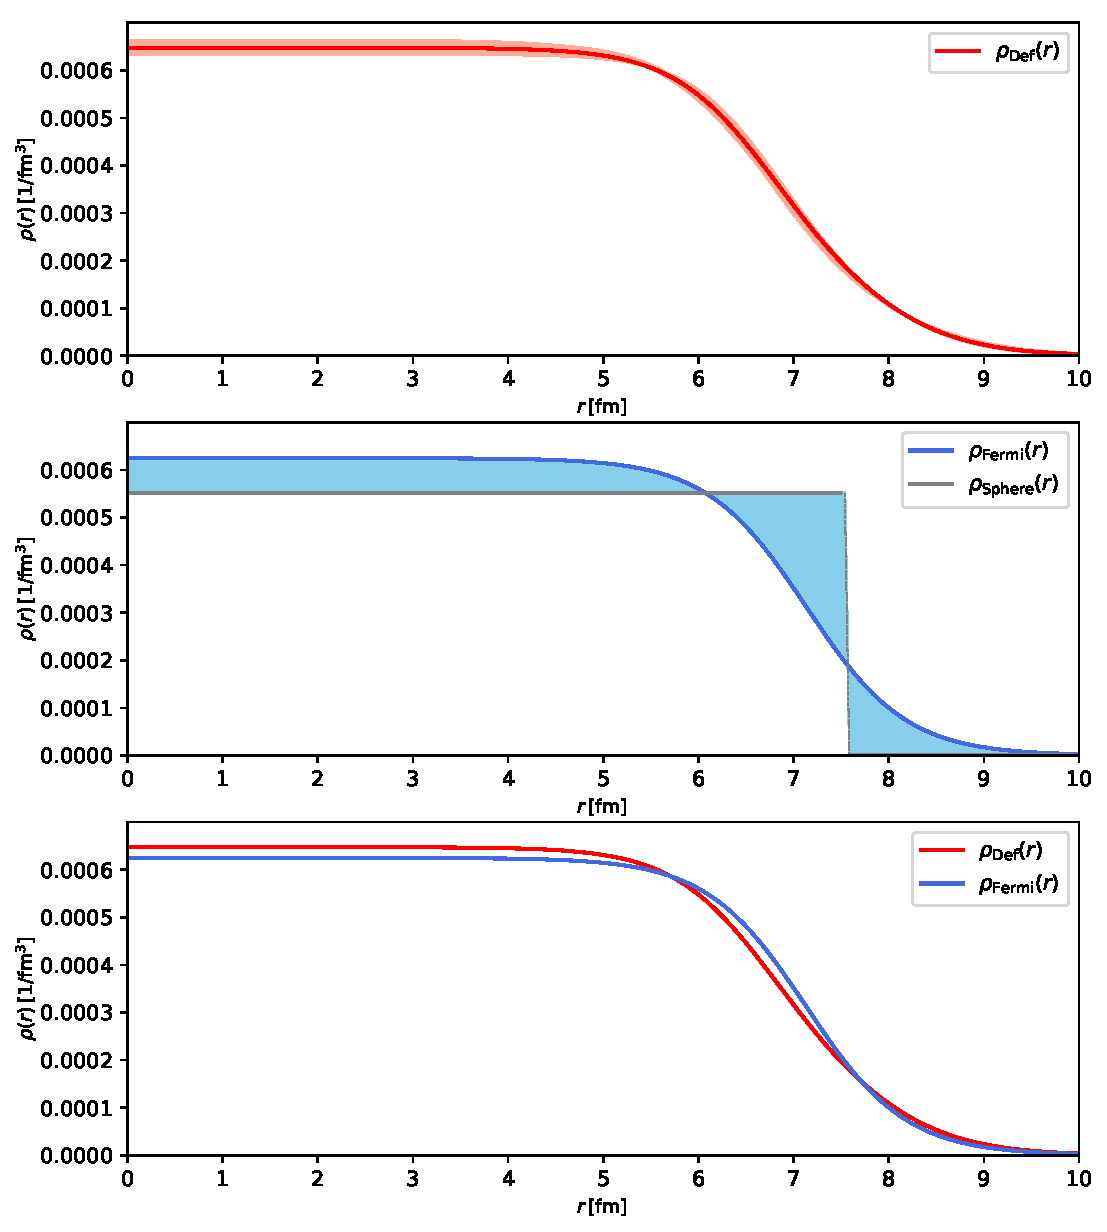
\includegraphics[width=\textwidth]{pics/chargeDistr.pdf}\\
\caption{\label{fig:charge distr.}\\
Upper figure: Deformed Fermi distribution for $^{238}$U, where the parameters and their uncertainties are taken from~\cite{kozhedub2008}. The light red border shows the uncertainties due to the parameters $a$, $\beta_2$, $\beta_4$, which is the remaining model uncertainty once the nuclear charge radius is fixed and which enables a reduced model uncertainty in the finite nuclear size $g$-facor correction.\\
Middle figure: Normal Fermi distribution with $a=0.5234\,$fm and homogeneoulsy charged sphere with the same charge radius as the deformed Fermi distribution. The difference (in light orange) is the conventional model uncertainty of the unclear charge distribution, which is larger as in the upper figure.\\
Lower figure: Comparison of normal and deformed Fermi distribution with the same RMS radius. The difference causes the nuclear deformation effect.}
\end{figure*}
% charge distribution figure end
%
\section{Non-perturbative analysis of nuclear shape effects}
In this work, we focus on quadrupole deformations and beyond, since atomic nuclei do not possess static dipole moments. Here, the deformed Fermi distribution
\begin{equation}
\rho_{ca\beta}(r,\vartheta)=\cfrac{N}{1+\text{exp}(\frac{r-c(1+\beta_2 \text{Y}_{20}(\vartheta)+\beta_4 \text{Y}_{40}(\vartheta))}{a})}
\label{eq:deffermi}
\end{equation}
as a model of the nuclear charge distribution has proved to be very successful, e.g. in heavy muonic atom spectroscopy with deformed nuclei \cite{hitlin1970,tanaka1984}; the normal Fermi distribution (${\beta_i}{=}{0}$) has also been used in electron-nucleus scattering experiments determining the nuclear charge distribution \cite{hahn1956}. Here, $a$ is a skin thickness parameter and $c$ the half-density radius, while $\beta_2$, $\beta_4$ are deformation parameters. $\text{Y}_{lm}(\vartheta,\varphi)$ are the spherical harmonics and $\text{Y}_{l0}(\vartheta)$ depend only on the polar angle $\vartheta$, and not on the azimuthal angle $\varphi$. The normalization constant $N$ is determined by the condition
\begin{equation}
\int \text{d}^3r\, \rho_{ca\beta}(r,\vartheta)=1.
\end{equation}
%
% begin table with comarison non-pert vs. eff-rad
\begin{table}[b]
\caption{\label{tab:spline}%
Comparison of the ND $g$~factor correction obtained by the ERM with the analytical expressions from Eqs.~\eqref{eq:efs} and \eqref{eq:radius} ($\delta g_{\text{ND}}^{(\text{eff,A})}$), by the ERM with effective radius and corresponding energy correction calculated numerically ($\delta g_{\text{ND}}^{(\text{eff,N})}$) and non-perturbatively by direct numerical calculations ($\delta g_{\text{ND}}^{(\text{num})}$) for several isotopes. $R_N$ is the RMS nuclear electric charge radius from literature \cite{Angeli2013} and $\beta_2$ is the parameter of the deformed Fermi distribution (\ref{eq:deffermi}). $\beta_4 \approx 0$ is assumed, according to~\cite{Moller1995}. All methods, as well as the procedure for obtaining the parameters of the deformed Fermi distribution, are described in the text.
}
\centering
\begin{tabular}{lccccc}
 &$R{\scriptstyle _N(\text{fm})}$& $\beta_2$ & $\delta g_{\text{ND}}^{(\text{eff,A})}$ & $\delta g_{\text{ND}}^{(\text{eff,N})}$ & $\delta g_{\text{ND}}^{(\text{num})}$\\
\hline\\[-5pt]
$^{\phantom{0}58}_{\phantom{0}26}$Fe & 3.775 & 0.273 & ${\text{-}}{2.19}{\scriptstyle\times}{10^{\text{-}11}}$ &${\text{-}}{2.02}{\scriptstyle\times}{10^{\text{-}11}}$&${\text{-}}{2.11}{\scriptstyle\times}{10^{\text{-}11}}$\\[4pt]
$^{\phantom{0}82}_{\phantom{0}38}$Sr & 4.246 & 0.263 & ${\text{-}}{3.56}{\scriptstyle\times}{10^{\text{-}10}}$ &${\text{-}}{3.16}{\scriptstyle\times}{10^{\text{-}10}}$&${\text{-}}{3.27}{\scriptstyle\times}{10^{\text{-}10}}$\\[4pt]
$^{\phantom{0}98}_{\phantom{0}44}$Ru & 4.423 & 0.194 & ${\text{-}}{6.00}{\scriptstyle\times}{10^{\text{-}10}}$ &${\text{-}}{5.25}{\scriptstyle\times}{10^{\text{-}10}}$&${\text{-}}{5.41}{\scriptstyle\times}{10^{\text{-}10}}$\\[4pt]
$^{116}_{\phantom{0}48}$Cd           & 4.628 & 0.189 & ${\text{-}}{1.20}{\scriptstyle\times}{10^{\text{-}9\phantom{0}}}$ &${\text{-}}{1.04}{\scriptstyle\times}{10^{\text{-}9\phantom{0}}}$&${\text{-}}{1.07}{\scriptstyle\times}{10^{\text{-}9\phantom{0}}}$\\[4pt]
$^{116}_{\phantom{0}50}$Sn           & 4.627 & 0.108 & ${\text{-}}{5.11}{\scriptstyle\times}{10^{\text{-}10}}$ &${\text{-}}{4.42}{\scriptstyle\times}{10^{\text{-}10}}$&${\text{-}}{4.55}{\scriptstyle\times}{10^{\text{-}10}}$\\[4pt]
$^{134}_{\phantom{0}54}$Xe           & 4.792 & 0.113 & ${\text{-}}{1.09}{\scriptstyle\times}{10^{\text{-}9\phantom{0}}}$ &${\text{-}}{9.36}{\scriptstyle\times}{10^{\text{-}10}}$&${\text{-}}{9.62}{\scriptstyle\times}{10^{\text{-}10}}$\\[4pt]
$^{152}_{\phantom{0}64}$Gd           & 5.082 & 0.202 & ${\text{-}}{1.53}{\scriptstyle\times}{10^{\text{-}8\phantom{0}}}$ &${\text{-}}{1.29}{\scriptstyle\times}{10^{\text{-}8\phantom{0}}}$&${\text{-}}{1.32}{\scriptstyle\times}{10^{\text{-}8\phantom{0}}}$\\[4pt]
$^{208}_{\phantom{0}82}$Pb           & 5.501 & 0.061 & ${\text{-}}{1.35}{\scriptstyle\times}{10^{\text{-}8\phantom{0}}}$ &${\text{-}}{1.10}{\scriptstyle\times}{10^{\text{-}8\phantom{0}}}$&${\text{-}}{1.13}{\scriptstyle\times}{10^{\text{-}8\phantom{0}}}$\\[4pt]
$^{244}_{\phantom{0}94}$Pu           & 5.864 & 0.287 & ${\text{-}}{1.28}{\scriptstyle\times}{10^{\text{-}6\phantom{0}}}$ &${\text{-}}{1.03}{\scriptstyle\times}{10^{\text{-}6\phantom{0}}}$&${\text{-}}{1.05}{\scriptstyle\times}{10^{\text{-}6\phantom{0}}}$\\[4pt]
$^{248}_{\phantom{0}96}$Cm           & 5.825 & 0.299 & ${\text{-}}{1.70}{\scriptstyle\times}{10^{\text{-}6\phantom{0}}}$ &${\text{-}}{1.36}{\scriptstyle\times}{10^{\text{-}6\phantom{0}}}$&${\text{-}}{1.39}{\scriptstyle\times}{10^{\text{-}6\phantom{0}}}$\\[4pt]
\end{tabular}
\end{table}
% end table
%
For the deformed Fermi distribution~(\ref{eq:deffermi}) with a fixed charge number $Z$, the $g$~factor (\ref{eq:gfacgs}) is completely determined by the parameters $c$, $a$ and $\beta_i$, and therefore can be written for the ground state as
\begin{equation}
g = g_{\text{point}} + \delta g^{(ca\beta)}_{\text{FS}},
\label{eq:finiteDef}
\end{equation}
where $\delta g^{(ca\beta)}_{\text{FS}}$ is the finite size correction depending on the parameters $c$, $a$, and $\beta_i$. In \cite{jacek2012}, the ND correction to the bound electron $g$~factor is defined as the difference of the finite size effect due a deformed charge distribution and due to a symmetric charge distribution (i.e. ${\beta_i}{=}{0}$) with the same nuclear radius as
\begin{equation}
\delta g_{\text{ND}}=\delta g^{(c_1a\beta)}_{\text{FS}} - \delta g^{(c_2a0)}_{\text{FS}},
\label{eq:defdgnd}
\end{equation}
where $a=2.3\,\text{fm}/(4\text{ln}(3))$, and $c_i$ are determined such that $\sqrt{\left<r^2\right>_{\rho}}$ of the corresponding charge distribution agrees with the root-mean-square (RMS) values from literature \cite{Angeli2013}. The $n$-th moment of a charge distribution $\rho(\vec{r}\,)$ is defined as
\begin{equation}
\left< r^n \right>_{\rho} = \int \text{d}^3r\,\, r^n \rho(\vec{r}\,).
\label{eq:nmoment}
\end{equation}
Values for the deformation parameter $\beta_2$ can be obtained by literature values of the reduced E2-transition probabilities from a nuclear state $2^+_i$ to the ground state $0^+$ via~\cite{Trager}:
\begin{equation}
\beta_2 = \frac{4\pi}{3Z|e|\sqrt{5\left< r^2\right>_{\rho} /3}}\left[ \sum_i B(E2;0^+\rightarrow 2_i^+) \right]^{1/2}
\label{eq:beta}
\end{equation}
From Eq.~(\ref{eq:defdgnd}) it is evident that the ND correction is a difference of two finite size effects and therefore especially sensitive on higher order effects. However, for high $Z$ it reaches the $10^{-6}$~level and therefore is very significant.

It was shown in~\cite{jacek2012} with the ERM \cite{Shabaev1993} that $\delta g_{\text{FS}}^{(ca\beta)}$ and therefore $\delta g_{\text{ND}}$ mainly depends on the moments $\left< r^2 \right>_{\rho}$ and $\left< r^4 \right>_{\rho}$. $\delta g_{\text{ND}}$ can be calculated with the formula~\cite{Karshenboim2005}
\begin{equation}
\delta g^{(ca\beta)}_{\text{FS}}=\frac{4}{3}\frac{\partial E_{\text{FS}}(c,a,\beta)}{\partial m_e},
\label{eq:effrad}
\end{equation}
which is a direct consequence of Eq.~(\ref{eq:deriv}) and where $E_{\text{FS}}(c,a,\beta)$ is the energy correction due to $\rho_{ca\beta}(r,\vartheta)$ compared to the point like nucleus.
The effective radius~$R$ is defined as the radius of a homogeneously charged sphere with the same energy correction $E^{(\text{sph})}_{\text{FS}}(R)$ as the deformed Fermi distribution via
\begin{equation}
E^{(\text{sph})}_{\text{FS}}(R) = E_{\text{FS}}(c,a,\beta).
\label{eq:effradNum}
\end{equation}
The energy correction can be approximated~\cite{Shabaev1993} as
\begin{equation}
E^{(\text{sph})}_{\text{FS}}(R)\approx\frac{(Z\alpha)^2}{10}\left[{1}{+}(Z\alpha)^2f(Z\alpha) \right](2Z\alpha R m_e)^{2\gamma}m_e.
\label{eq:efs}
\end{equation}
Here, $f(x)=1.380-0.162x+1.612x^2$ and the effective radius is approximately
\small
\begin{equation}
R\approx\sqrt{\frac{5}{3}\left<r^2\right>_{\rho_{ca\beta}}\left[ 1-\frac{3}{4}(Z\alpha)^2 \left( \frac{3}{25}\cfrac{\left<r^4\right>_{\rho_{ca\beta}}}{\left<r^2\right>^2_{\rho_{ca\beta}}}-\frac{1}{7} \right) \right]}.
\label{eq:radius}
\end{equation}
\normalsize
While \eqref{eq:effrad} is exact for an arbitrary central potential, provided that $E_{\text{FS}}$ is known exactly, \eqref{eq:efs} is an approximation derived under the assumption of the difference between point-like and extended potential being a perturbation. The calculation of the ND correction to the bound electron $g$~factor via the effective radius approach therefore relies on a perturbative evaluation of the energy derivative in Eq.~(\ref{eq:effrad}) and is limited by the accuracy of the finite size corrections.

In this work, the ND $g$-factor correction is calculated with three methods:
Firstly, with the previously used analytical ERM described above. Secondly, with a numerical ERM, where instead of the approximative Eqs.~\eqref{eq:efs} and \eqref{eq:radius}, Eq.~\eqref{eq:effradNum} is solved numerically for $R$ and the ND $g$-factor correction is obtained by using Eq.~\eqref{eq:gfacgs} with the wave functions of the corresponding charged sphere.
Finally, we also calculate $\delta g_{\text{ND}}$ non-perturbatively by solving the Dirac equation (\ref{eq:diraceq_nucldef}) numerically with the dual kinetic balance method~\cite{dualkinetic} for the potential (\ref{eq:potdef}), including all finite size effects due to the deformed charge distribution $\rho_{ca\beta}(r,\vartheta)$. Then, the $g$~factors needed in Eq.~(\ref{eq:defdgnd}) for the ND correction can be obtained by numerical integration of the wave functions in Eq.~(\ref{eq:gfacgs}). Alternatively, the derivative of the energies in Eq.~(\ref{eq:deriv}) can be calculated numerically as 
\begin{equation}
\frac{\partial E_{n\kappa}}{\partial m_e} \approx \frac{E_{n\kappa}^{(m_e+\delta m)}-E_{n\kappa}^{(m_e-\delta m)}}{2 \delta m},
\end{equation}
with a suitable ${\delta m / m_e}{\ll}{1}$. Here, $E_{n\kappa}^{(m_i)}$ stands for the binding energy obtained by solving the Dirac equation with the electron mass replaced by $m_i$. We find both methods in excellent agreement.

\begin{figure*}
  \centering
  \begin{minipage}[b]{\textwidth}
    \centering
    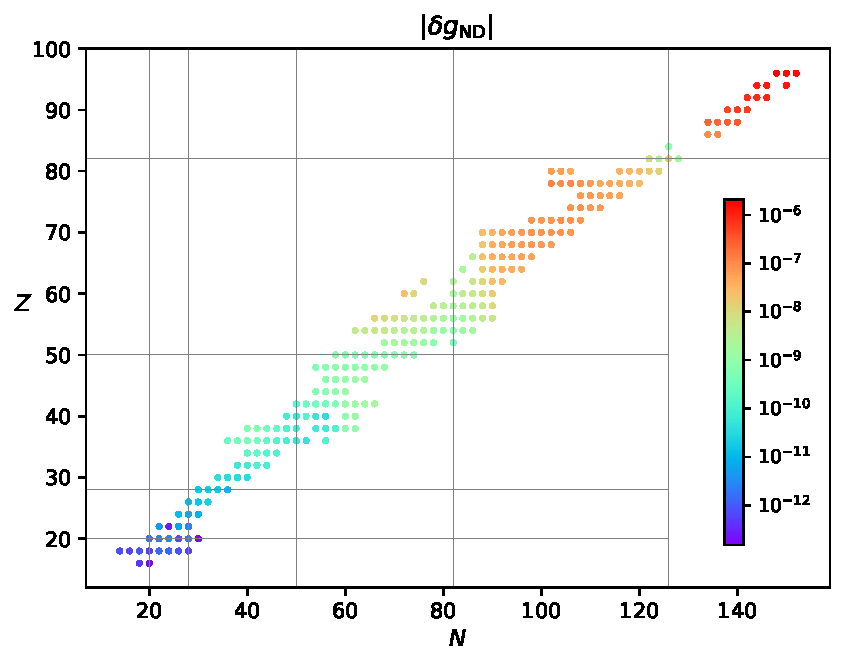
\includegraphics[width=0.94\textwidth]{pics/dgnuclchart.pdf}\\
    $\qquad \, \,$(a)
  \end{minipage}
  \hfill
  \begin{minipage}[b]{\textwidth}
     \centering
    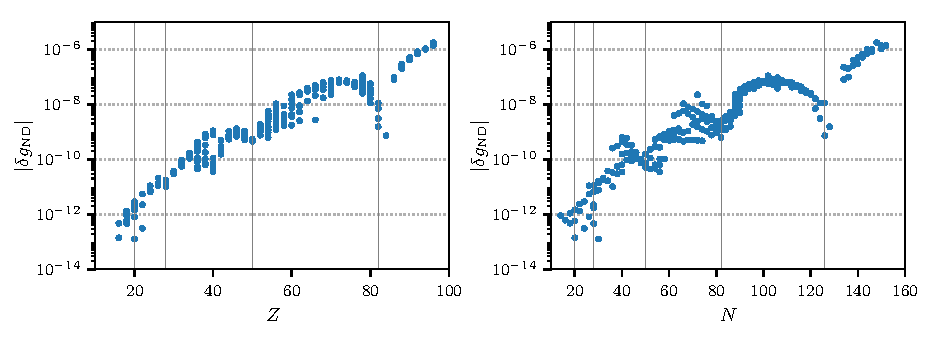
\includegraphics[width=0.99\textwidth]{pics/dgZN.pdf}\\
    \hspace{1.3cm}(b)\hspace{6.7cm}(c)
    \caption{\label{fig:dg}(Color online) Nuclear chart with charge number $Z$ and neutron number $N$, where the grey lines indicate the magic numbers 20, 28, 50, 82, and 126. The points represent even-even nuclei, where their color in (a) displays the ND $g$-factor correction $\delta g_{\text{ND}}$, calculated with the numerical, non-perturbative approach, which takes particularly low values around the magic numbers and larger values in between. The two lower figures show $\delta g_{\text{ND}}$ with the numerical approach for the considered even-even nuclei as a function of only the charge number $Z$ (b) and of only the neutron number $N$ (c), respectively. See~\cite{michel2015} for an evaluation with the previously used perturbative method. The vertical solid grey lines are the nuclear magic numbers, which show that filled proton, as well as neutron shells, reduce $\delta g_{\text{ND}}$.}
  \end{minipage}
\end{figure*}

We calculated the ND $g$-factor correction for a wide range of even-even, both in the proton and neutron number, and therefore spinless nuclei with charge numbers between 16 and 96 using the deformed Fermi distribution from~Eq.~(\ref{eq:deffermi}) with parameters $a$, $c$, and $\beta$ obtained as described below Eq.~(\ref{eq:defdgnd}). The required RMS values for the nuclear charge radius are taken from~\cite{Angeli2013} and the reduced transition probabilities needed for the calculation of $\beta$ via (\ref{eq:beta}) from \cite{ENSDF}. The resulting values for $|\delta g_{\text{ND}}|$, obtained by the non-perturbative method, are shown in Fig.~\ref{fig:dg} as a function of the charge number $Z$ and the neutron number $N$. If proton or neutron number is in the proximity of a nuclear magic number 2, 8, 20, 28, 50, 82, and 126, which corresponds to a filled proton or neutron shell \cite{Ring}, the nuclear shell closure effects also transfer to the bound electron $g$~factor, and the ND correction is reduced~\cite{michel2015}. In Table \ref{tab:spline}, a comparison between our numerical approaches and the analytical ERM from \cite{jacek2012} is shown.

Now, let us discuss the main causes for the disagreement of the results as presented in Table~\ref{tab:spline}. Both Eqs.~\eqref{eq:efs} and~\eqref{eq:radius} are approximations derived by perturbation theory, which affects the accuracy of the analytical ERM ($\delta g_{\text{ND}}^{(\text{eff,A})}$). Eq.~\eqref{eq:efs} has an estimated relative uncertainty ${\scriptstyle\lesssim}\,0.2\,\%$~\cite{Shabaev1993} and \eqref{eq:radius} uses only the second and fourth moment of the nuclear charge distribution for finding the effective radius. Also, it was shown in~\cite{karshenboim2018} that the analytical ERM for arbitrary charge distributions is incomplete in order $(Z\alpha)^2m_e(Z\alpha m_e R_N)^3$, where $R_N$ is the nuclear RMS charge radius. Furthermore, even if the effective radius is calculated without approximations according to Eq.~\eqref{eq:effradNum}, the wave functions of the corresponding homogeneously charged sphere differ slightly from the ones of the deformed Fermi distribution with the same binding energy. This affects values of the $g$~factor and explains the difference between the numerical ERM ($\delta g_{\text{ND}}^{(\text{eff,N})}$) and the direct numerical calculations ($\delta g_{\text{ND}}^{(\text{num})}$). 
Finally, being a difference of two small finite-nuclear-size corrections, the ND correction can exhibit enhanced sensitivity on the uncertainty of the ERM.
From Table~\ref{tab:spline}, we conclude that for high $Z$, the difference between analytical ERM and non-perturbative calculations is mainly due to the approximations in Eqs.~\eqref{eq:efs} and~\eqref{eq:radius}.

Concluding, the analytical ERM proved to be a good order-of-magnitude estimate of the ND correction, but for high-precision calculations, non-perturbative methods beyond the ERM and without an expansion in $Z\alpha$ or $Z\alpha\, m_e\, R_N$ are indispensable. Convergence of the numerical methods was checked by varying numerical parameters and using various grids, and the obtained accuracy permits the consideration of nuclear size and shape with an accuracy level much higher than the differences to the perturbative method.

\begin{table}[t]
\caption{\label{tab:uranium}%
Comparison of the finite nuclear size correction for the normal Fermi distribution $\delta g_{\text{FS}}^{\text{(Fermi)}}$ and the deformed Fermi distribution $\delta g^{(ca\beta)}_{\text{FS}}$, evaluated with the effective radius method (ERM) and numerically. The number in the first and second parenthesis is the uncertainty due to the RMS charge radius and the model uncertainty, respectively. Parameters are taken from Ref.~\cite{kozhedub2008}.
}
\centering
\begin{tabular}{lcc}
&ERM&Numerical\\\hline\\
$\delta g_{\text{FS}}^{\text{(Fermi)}}$&$1.2860(11)(31)\times 10^{-3}$&$1.2739(11)(25)\times 10^{-3}$\\[0.4cm]
$\delta g^{(ca\beta)}_{\text{FS}}$&$1.2852(11)(9)\phantom{0}\times 10^{-3}$&$1.2733(11)(7)\phantom{0}\times 10^{-3}$
\end{tabular}
\end{table}
Previously, the uncertainty of the finite nuclear size correction was commonly estimated as the difference between the Fermi distribution and a homogeneously charged sphere, which is a very conservative estimate~\cite{Shabaev2006}. If the finite size correction is calculated as $\delta g^{(ca\beta)}_{\text{FS}}$ from Eq.~\eqref{eq:finiteDef} including deformation effects, the remaining model uncertainty is reduced to the difference between the deformed Fermi distribution and the true, unknown nuclear charge distribution.
As a consequence, precise values for $c$, $a$, and $\beta$ need to be known, e.g. from muonic atoms spectroscopy~\cite{Close1978,hitlin1970}, along with their error bars, which are needed to estimate the difference between deformed Fermi and true charge distribution. 
The reduction of model uncertainties is demonstrated in Fig~\ref{fig:charge distr.}. Here, the averaged charge distribution for the deformed Fermi distribution with parameters from~\cite{kozhedub2008} is shown along with errorbars due to the uncertainties in $a$, $c$, $\beta_2$, and $\beta_4$. For comparison, the conventional way of estimating the model dependence is also demonstrated by showing difference between the normal Fermi and charged sphere charge distribution.

For values of the RMS radius, $a$, $\beta_2$, and $\beta_4$ of $^{238}$U  taken from Ref.~\cite{kozhedub2008}, it is shown it Table~\ref{tab:uranium} that accounting for the deformation effects reduces the uncertainty of the finite size correction by more than a factor of two. Also, it shows that the difference of the ERM and the all-order numerical method is larger than the uncertainty due to nuclear parameters.

In total, the ND $g$-factor correction was calculated non-perturbatively for a wide range of nuclei by using quadrupole deformations estimated from nuclear data.
By comparing the previously used perturbative ERM and the all-order numerical approach, it was shown that the contributions of the non-perturbative effects can amount up to the $20\,\%$ level.
In the low-$Z$ regime, the ND corrections can safely be neglected, especially for the ions considered in \cite{Sturm2014}. However, considering a ND correction up to the parts-per-million level and an expected parts-per-billion accuracy, or even below, for the $g$-factor experiments with high-$Z$ nuclei, in this case an all-order treatment is indispensible. 
For hydrogenlike Uranium, it was shown that inclusion of deformation effects leads to reduced uncertainties in the theoretical prediction of the finite nuclear size correction.
On the other hand, since he distribution of electric charge inside the nucleus is a major theoretical uncertainty for $g$~factors with heavy nuclei, the extraction of information thereon from experiments is possible. Our work demonstrates the required accurate mapping of arbitrary nuclear charge distributions to corresponding $g$~factors.
\newpage
\section{Summary}
At first, in this Chapter, the following known results are summarized:
\begin{enumerate}
\item For spinless nuclei, the angular dependence of the interaction energy averaged out and the bound electron is exposed to a averaged, spherically symmetric nuclear potential.
\item For these spherically symmetric potentials, the bound electron $g$ factor can be obtained by solving the Dirac equation and then performing radial integrals or deriving the binding energy by the electron mass
\item Deformed charge distributions cause a nuclear shape or nuclear deformation effect on the $g$ factor, which can be calculated perturbatively with the effective radius method according to~\cite{jacek2012}.
\end{enumerate}
From thereon, the following new results are presented in this thesis:
\begin{itemize}
\item The nuclear shape correction is calculated without using the perturbative effective radius method. Instead, the averaged potential is calculated numerically starting from a given deformed charge distribution. Then, finite basis set methods are used to solve the Dirac equation numerically in this potential and the integrals and energy derivatives for the bound electron $g$ factor are performed numerically, as well. Thereby, nuclear deformation effects on the bound electron $g$ factor are obtained non-perturbatively.
\item Results for a wide range of nuclei were presented using the non-perturbative method. It was shown that the results for the deformation effects of the previously used perturbative effective radius method differ from the non-perturbative results on the $20\%$-level
\item For the example of Uranium-238, it was shown with available parameters on the deformed charge distribution that the uncertainty of the finite nuclear size effect can be reduced by a factor of two by considering deformation effects. Furthermore it was demonstrated that the non-perturbative method is needed for acurate results.
\end{itemize}


  
  %\chapter{Nuclear shape g factor papers}





  
  %\chapter{Vacuum polarization corrections to the bound muon g factor in $\mu$-He}
\label{ch:muongfac}
 








  
  \chapter{Hyperfine structure of muonic atoms}
\label{ch:muonic_atoms}
This chapter is devoted to the prediction of the level structure and transition probabilities in muonic atoms with focus on high nuclear charge numbers. Compared to conventional atomic electrons, the much higher muon mass reduces the length- and  increases the energy scales by the muon-electron mass ratio. Thereby, all finite nuclear size and shape effects are much more important and also excited nuclear states have to be taken into account.\\
This chapter is organized in the following way:\\
At first, a motivation for the need for new structure calculations is given in Section~\ref{sec:muon_motivation} by comparing to existing methods and by pointing new experiments in the field out, which use the results presented in this thesis.\\
Afterwards, the theoretical framework and implementation of several known effects is shown in Sections~\ref{sec:muon_framework} to~\ref{sec:muon_dynamic}, using finite basis set methods suitable for precision calculations and presenting results for selected nuclei.\\
In Sections~\ref{sec:muon_residualSO} and~\ref{sec:muon_quadUehl}, improved methods for calculating higher order effects in the electric hyperfine interactions are presented.\\
Finally, in Sections~\ref{sec:muon_re}, calculations in combination with experiments on isotopically pure Rhenium-185 are presented, including the extraction of the nuclear quadrupole moment by combining theoretical predictions and measurements of muonic transitions. \\
In Section~\ref{sec:muon_he}, precision calculations for the vacuum polarization corrections to the bound-muon $g$ factor in muonic Helium-4 are shown.

\section{Calculation of spectra for muonic atoms}
\subsection{Motivation}
\label{sec:muon_motivation}
Atomic nuclei are one of the building blocks of matter and therefore, information on their structure, like the distribution of electric charge inside the nucleus, is of intrinsic interest. Furthermore, the charge radii of atomic nuclei are of importance as an input parameter for the interpretation of other experiments. For example, radium atoms are a candidate for measuring atomic parity violation effects, but for this more accurate values of the radium charge radii are needed~\cite{wansbeek2012}.
There are several methods for extracting information on the nuclear charge distribution, i.e. the distribution of protons inside the atomic nucleus, like electron scattering~\cite{devries1987} or laser spectroscopy~\cite{wang2004,dewitte2007,mueller2007}. One method is also muonic atom spectroscopy. Here, a muon, which is a negatively charged elementary particle is brought in the proximity of an atomic nucleus. Then, the negatively charged muon forms bound states with the positively charged nucleus and radiation due to muonic transitions can be analyzed in order to obtain information on the nuclear charge distribution and measure quantities like nuclear charge radii and quadrupole moments.

Correspondingly, the theory of muonic atoms has been developed in order to describe the level structure and the probabilities for muonic transitions. The general approach is that for a given nuclear charge distribution, the spectrum of the corresponding muonic atom needs to be predicted. Then, vice versa, for a measured spectrum the nuclear charge distribution can be extracted. An overview of the different contributions to the energy levels of muonic atoms can be found in~\cite{BorieRinker1982}. Hitherto, the majority of analyses of the spectra of heavy muonic atoms used the computer programs \textit{MUON} and \textit{RURP}~\cite{rinker1979}. There are two main differences compared to the approach used in this thesis:
Firstly, the dual-kinetic-balance method~\cite{Shabaev2004} is used in this thesis. Being a finite basis set method, a approximation of the complete muon spectrum is obtained, i.e. bound states and positive as well as negative continuum states, including the effects of the finite nuclear charge distribution. Thereby, numerical summations over the complete muon spectrum are possible. This enables for example a complete treatment of the second order hyperfine interactions, as presented in Section~\ref{sec:muon_residualSO}.
Secondly, whereas in the \textit{MUON} and \textit{RURP} codes, the fine and hyperfine structure are calculated separately, in this thesis the calculations of the fine and hyperfine structure are performed at once, based on a given nuclear charge distribution, enabling improved analysis of the dependence of the muonic spectrum on parameters of the nuclear charge distribution.

Furthermore, there are new experiments on high $Z$ muonic atoms being performed by the muX-Collaboration at the Paul-Scherrer-Institute in Villigen, Switzerland~\cite{kirch2016}. One of the goals is to measure the charge radius for Radium, needed for experiments on atomic parity violations, as mentioned earlier in this Section. Furthermore, measurements on muonic atoms involving several nuclei will be or have been performed for the first time, involving isotopically pure Rhenium. The corresponding structure calculations for muonic Rhenium were performed during the work on this thesis, and results are presented in Section~\ref{sec:muon_re}.

\subsection{Theoretical framework}
\label{sec:muon_framework}
A muon is a charged elementary particle, which is in many aspects similar to the electron, in particular, it has the same electric charge, but it is ${\approx}\,{200}$ times heavier than the electron~\cite{codata}. When coming close to an atom, a muon can be captured by the nucleus and form a hydrogen-like muonic ion. This atomic system is commonly referred to as a muonic atom. The lifetime of the muon is big enough to be considered stable in the structure calculations of these muonic bound states.
The reason why muonic atoms, compared to conventional electronic atoms, are suitable for extraction information on nuclear structure is that the muon is about 207 times heavier than the electron. This can be seen by considering the ratio of the nuclear radius and the Bohr radius of the bound fermion, which is the typical length scale for the bound muon or electron. The larger this ratio is, the larger are nuclear finite size effects. The Bohr radius for a hydrogen-like atomic system with a bound fermion of mass $m_f$ and a nuclear charge number $Z$ reads as
\begin{equation}
r_B = \hbar / (m_f c Z \alpha),
\end{equation}
where $\hbar$ is the Planck's constant, $\alpha$ is the finestructure constant and $c$ is the speed of light in vacuum. In Table~\ref{tab:nucl_radii}, the nuclear radius, the Bohr radius for the corresponding electronic and muonic hydrogen-like ion, and their ratio is shown for a selection of nuclei, from very light to very heavy.
%
%
\begin{table}
\caption{\label{tab:nucl_radii}
Comparison of the ratio of nuclear charge radius $R_N$ to the Bohr radius $r_B$ of a bound electron or muon in the corresponding hydrogen-like atomic system for Hydrogen, Helium, Rhenium, and Uranium. If this ratio is small, the finite size of the nucleus does not influence the bound fermion significantly. On the other hand, if this ratio is on the order of 1, large finite nuclear size and nuclear structure effects can be expected. The nuclear charge radii are taken from~\cite{Angeli2013}.}
\centering
\begin{tabular}{ccccc}
Fermion type & Nucleus & $R_N$[fm]&$r_B$[fm]&$R_N/r_B$\\\hline\\[-5pt]
$e^-$&$^1_1$H&0.8783&$52917.721$&$1.660\times 10^{-5}$\\[3pt]
$\mu^-$&$^1_1$H&0.8783&$\phantom{11}255.928$&$3.432\times 10^{-3}$\\[15pt]
$e^-$&$^4_2$He&1.6755&$26458.861$&$6.332\times 10^{-5}$\\[3pt]
$\mu^-$&$^4_2$He&1.6755&$\phantom{11}127.964$&$1.309\times 10^{-2}$\\[15pt]
$e^-$&$^{185}_{\phantom{1}75}$Re&5.3596&$\phantom{11}705.570$&$7.596\times 10^{-3}$\\[3pt]
$\mu^-$&$^{185}_{\phantom{1}75}$Re&5.3596&$\phantom{1111}3.412$&$1.571\phantom{111111}$\\[15pt]
$e^-$&$^{238}_{\phantom{1}92}$U&5.8571&$\phantom{11}575.193$&$1.018\times 10^{-2}$\\[3pt]
$\mu^-$&$^{238}_{\phantom{1}92}$U&5.8571&$\phantom{1111}2.782$&$2.105\phantom{111111}$
\end{tabular}
\end{table}
%
%
It can be seen that, that for electronic atoms, the nucleus is generally a few orders of magnitude smaller compared to the extend of the electronic wave function, which is given by the Bohr radius, although for high $Z$, the electron is much closer to the nucleus due to the strong Coulomb attraction. Since the Bohr radius is inversely proportional to the mass of the bound fermion, the situation in muonic atomic systems is different. While for low $Z$, the extend of the muonic wave functions is still much larger than the nuclear radius, for high $Z$, the nuclear radius is actually larger than the muonic Bohr radius. This means the overlap between muonic wave functions and nucleus is large in this case. Also, a typical energy scale for hydrogen-like systems is the ground state binding energy from Eq.~\eqref{eq:finestructure_formula} for a point-like nucleus, which reads as
\begin{equation}
E_{0,\text{point}}=m_f c^2 (1-\sqrt{1-(Z\alpha)^2}),
\end{equation}
and is proportional the fermion mass. As a consequence, for muonic atoms and high charge numbers, muonic transitions can have an energy of several mega electronvolts and fine structure splitting can be on the order of several hundreds of kilo electronvolts. This is of the same order as excitation energies of nuclear rotational states~\cite{ENSDF} and therefore a nuclear model has to be used, which besides an extended charge distribution also contains the excited nuclear states of the ground state rotational band. Here, the symmetric rigid rotor model model for nuclei with axial symmetry has proved successful in describing heavy muonic atoms, e.g.~\cite{tanaka1984,hitlin1970,wu1969,Devons1995} and also is used in this thesis. The symmetric rigid rotor model is introduced in Appendix~\ref{app:rig_rotor}, where also the expressions for the nuclear wave functions in terms of Wigner D functions can be found. In the symmetric rigid rotor model, the nucleus is described by a charge distribution $\rho(\mathbf{r})$ given in the body fixed nuclear frame, and the Euler angles $\Omega=(\phi,\theta,\psi)$ describe its position in the laboratory frame. The rotational state of the nucleus $\left|IMK\right>$ is given by the total nuclear angular momentum quantum number $I$, its projection on the $z$ axis of the laboratory frame $M$ and on the $z$ axis of the body fixed frame $K$, where $K$ also corresponds to the ground state angular momentum. As derived in Chapter~\ref{ch:furry_pic}, the muonic bound states without radiative corrections can be obtained by solving the Dirac equation for the nuclear potential. The coupled system of muon as a Dirac particle and nucleus as a rigid rotor therefore is described by the eigenvalue equation
\begin{equation}
\text{H} \left(\left|N\right>\otimes \left|\mu\right>\right)= \left(\text{H}_{\text{N}} + \text{H}_\mu + V_{\text{el}}\right) \left(\left|N\right>\otimes \left|\mu\right>\right)= E \left(\left|N\right>\otimes \left|\mu\right>\right),
\label{eq:muon_htotal}
\end{equation}
where $H_{\text{N}}$ is the nuclear rigid rotor Hamiltonian, and ${H_\mu}{=}{\boldsymbol{\alpha} \cdot \mathbf{p} + \beta m_\mu}$ is the free Dirac Hamiltonian for the muon with momentum $\mathbf{p}$, and $\boldsymbol{\alpha}$ and $\beta$ are the four Dirac matrices. $\left|N\right>$ is the nuclear state and $\left|\mu\right>$ is the muon state. Following Eq.~\eqref{eq:furry_elPot}, the electric potential energy between muon and nuclear charge distribution reads as
\begin{equation}
\label{eq:muon_elInteract}
V_{\text{el}}(\mathbf{r}_\mu^\prime)=-Z\alpha \int \mathrm{d}^3\mathbf{r}_N^\prime \frac{\rho(\mathbf{r}_N^\prime)}{|\mathbf{r}_\mu^\prime-\mathbf{r}_N^\prime|}.
\end{equation}
It is important to recall, that the nuclear charge distribution is given in the body fixed nuclear frame, thus the integration in Eq.~\eqref{eq:muon_elInteract} in most conveniently performed in this frame. The resulting expression in dependence of the position of the muon, however, is needed in the laboratory frame. Therefore, in the following, a multipole expansion of Eq.~\eqref{eq:muon_elInteract} is performed, and the result is given as a function of the muon position in the laboratory frame and the Euler angles describing the orientation of the nuclear frame. Here, vectors are written is spherical components as $\mathbf{r}_i = (r_i,\vartheta_i,\varphi_i)$ in the laboratory frame and as $\mathbf{r}_i^\prime = (r_i^\prime,\vartheta_i^\prime,\varphi_i^\prime)$ in the body-fixed nuclear frame. Since rotations do not change the absolute value of rotations, it holds that $r_i^\prime = r_i$.\\

With the multipole expansion of the Coulomb potential~\cite{jackson1999}
\begin{equation}
\frac{1}{|\mathbf{r}_\mu^{\,\prime}-\mathbf{r}_N^{\,\prime}|}=\sum_{l=0}^\infty \frac{r_<^l}{r_>^{l+1}}\sum_{m=-l}^l  \text{C}^*_{lm}(\vartheta_N^{\prime},\varphi_N^{\prime})\text{C}_{lm}(\vartheta_\mu^\prime,\varphi_\mu^\prime),
\end{equation}
where $r_<:=\min (r_\mu,r_N)$, $r_>:=\max (r_\mu,r_N)$, the electric potential~\eqref{eq:muon_elInteract} can be written as
\begin{align}
V_{\text{el}}(\mathbf{r}_\mu^{\,\prime})=&\sum_{l,m}-Z\alpha \left[ \int \text{d}^3r^{\prime}_N \frac{r_<^l}{r_>^{l+1}}\text{C}^*_{lm}(\vartheta_N^{\prime},\varphi_N^{\prime})\rho(\mathbf{r}_N^{\,\prime})\right]\notag\\
&\,\times\text{C}_{lm}(\vartheta_\mu^{\prime},\varphi_\mu^\prime),
\end{align}
where ${\text{C}_{lm}(\vartheta,\varphi)}{=}{\sqrt{4\pi/(2l+1)}\text{Y}_{lm}(\vartheta,\varphi)}$ are the normalized spherical harmonics.
For axially symmetric charge distributions, only the ${m}{=}{0}$-terms are non-zero after integrating over the charge distribution. The dependency on the muonic angular variables can be transformed to the laboratory system using the Euler angles by
\begin{equation}
\text{P}_{l}(\cos\vartheta_\mu^\prime)=
 \sum_{m=-l}^l C^*_{lm}(\theta,\phi)C_{lm}(\vartheta_\mu,\varphi_\mu),
\end{equation}
which is a special case of Eq.~\eqref{eq:rot_sphHarm}.
Thereby, the potential as a function of the Euler angles and the muon's position in the laboratory frame reads
\begin{align}
V_{\text{el}}(\mathbf{r}_\mu,\phi,\theta)=&\sum_{l=0}^\infty-Z\alpha \left[ \int \text{d}^3\mathbf{r}^{\prime}_N \frac{r_<^l}{r_>^{l+1}}\text{P}_{l}(\cos \vartheta_N^{\prime})\rho(\mathbf{r}_N^{\,\prime})\right]\sum_{m=-l}^l \text{C}^*_{lm}(\theta,\phi)\text{C}_{lm}(\vartheta_\mu,\varphi_\mu).\notag\\
\eqqcolon &\sum_{l=0}^\infty Q_{\text{el}}^{(l)}(r_\mu)\sum_{m=-l}^lC^*_{lm}(\theta,\phi)C_{lm}(\vartheta_\mu,\varphi_\mu)&\notag\\
\eqqcolon& \sum_{l=0}^\infty V^{(l)}_{\text{el}}(\mathbf{r}_\mu,\phi,\theta),
\label{eq:defmulti}
\end{align}
where $Q_{\text{el}}^{(l)}(r_\mu)$ describe the radial distribution of the multipole moments and the dependency on the muonic angles and the Euler angles is in form of a scalar product of spherical tensor operators. This means, as expected the interaction energy does only depend on the relative orientation of the muon with respect to the body fixed nuclear $z^\prime$ axis.

Most nuclei turn out to be symmetric with respect to reflection in the $(x^\prime ,y^\prime)$-plane~\cite{zickendraht1991}. This results in only even-$l$ terms in Eq.~\eqref{eq:defmulti} being non-zero, thus the first to terms are the monopole term $l=0$ and the quadrupole term $l=2$. The next term would be the $l=4$ hexadecapole terms, however, usually, higher order terms are not needed for the correct description of the hyperfine level structure. It follows from Eq.~\eqref{eq:defmulti}, that the monopole terms only depends on the muonic radial variable, since it can be written as
\begin{equation}
V_{\text{el}}^{(0)}(r_\mu)=-Z\alpha \int\text{d}^3\mathbf{r}_N^\prime \frac{\rho(\mathbf{r}_N^\prime)}{r_>}.
\end{equation} 
In fact, the $l=0$ terms is the averaged nuclear potential already derived in Eq.~\eqref{eq:gfac_monopole} in the previous chapter on the $g$ factor of spinless nuclei. As a consequence, the $l=0$-term can be used as a potential in the spherically symmetric Dirac equation to define the unperturbed muonic states as
\begin{equation}
\label{eq:muonicEn}
\left(\boldsymbol{\alpha} \cdot \mathbf{p} + \beta m_\mu + V_{\text{el}}^{(0)}(r_\mu) \right) \left|n\kappa m\right> = E_{n\kappa}\left|n\kappa m\right>.
\end{equation}
The unperturbed nuclear states are the rigid rotor states from Eq.~\eqref{app:rigidRot_state} with
\begin{equation}
\label{eq:nuclEn}
\text{H}_N \left|IMK\right> = E_N \left|IMK\right>,
\end{equation}
where the excitation energies of the nuclear rotational states are typically taken from experiment~\cite{ENSDF}, and not parametrized by the moment of inertia from Eq.~\eqref{eq:rig_rotorEn}.
The $l=2$ quadrupole term couples nuclear and muonic degrees of freedom and is treated in perturbation theory in Sections~\ref{sec:elQuad1},~\ref{sec:muon_dynamic}, and~\ref{sec:muon_residualSO}. The multipole interaction from Eq.~\eqref{eq:defmulti} in general, and the quadrupole interaction with $l=2$ in particular has the structure of a scalar product of two irreducible tensor operators, as defined in Eq.~\eqref{app:tensor_scalarProd}. One operator acts on the nuclear angular variables, i.e. the Euler angles, and one on the muonic angular variables.
For these types of operators, the calculation of expectation values can be simplified by using the theory of irreducible tensor operators, as described in Appendix~\ref{app:ang_theo}. For applying formula~\eqref{app:reducedMatEl_expectation}. Therefore, states of defined total angular momentum have to be considered as
\begin{equation}
\label{eq:totalState}
\left| FM\,IKj(\kappa)\right> = \sum_{M_N, m}\text{C}^{FM}_{IM_N\,jm}\left|IM_NK\right>\,\left|n\kappa m\right>
\end{equation}
with total angular momentum $F$, nuclear angular momentum $I$ and muonic angular momentum $j$ are defined. The muonic angular momentum $j$ is already composed out of the orbital angular momentum $l$ and the spin angular momentum, as described in Eq.~\eqref{eq:ansatz_dirac}. The total energy of the muon-nucleus system can be calculated as the sum of nuclear energy $E_N$ from Eq.~\eqref{eq:nuclEn}, the muonic energy from Eq.~\eqref{eq:muonicEn} and the expactation value of the quadrupole interaction $\left<V_{\text{el}}^{(2)}\right>$ from Eq.~\eqref{eq:defmulti}.

\subsection{Fine and first order hyperfine structure}
\label{sec:muon_finestructure}
In this Section, the solution of the Dirac equation for the muon will be discussed, in particular the effects of vacuum polarization in Uehling approximation, recoil corrections, electron screening are implemented, using known methods. Especially, the usage of the dual-kinetic-balance method~\cite{Shabaev2004} in the framework of muonic atoms is presented. In the following, the first order hyperfine structure is considered. Results are presented for muonic $^{205}$Bi, $^{147}$Sm, and $^{89}$Zr. This Section follows~\cite{michel2017}, which was published in the framework of this thesis.

\subsubsection{Finite nuclear size corrections}
\label{sec:radialEq}
%The total Hamiltonian for a muon bound to a nucleus can be written as a sum of nuclear, muonic, and interaction Hamiltonian~\cite{Devons1995}. Thus, we consider the Hamiltonian
%\begin{equation}
%H = H_{N} + H^{(0)}_{\mu} + H_{\mu - N},
%\end{equation}
%with the nuclear Hamiltonian $H_{N}$, the Dirac Hamiltonian $H^{(0)}_{\mu}$ for the free muon, and the interaction Hamiltonian $H_{\mu - N}$. The nucleus is described in the rotational model, i.e. in a state with well defined angular momentum and charge- and current density in the body fixed nuclear frame~\cite{kozhedub2008}. As a next step, the interaction between the bound muon and the atomic nucleus is expanded, where electric and magnetic interactions are taken into account. The interaction Hamiltonian is
%\begin{equation}
%\label{eq:Hint}
%H_{\mu - N} = H_{E} + H_{M}
%\end{equation}
%where the electric part reads
%\begin{equation}
%\label{eq:elInt}
%H_{E}= - \alpha \int \mathrm{d}V^{\prime}\, \frac{\rho (\vec{r}^{\,\prime})}{|\vec{r}_{\mu}-\vec{r}^{\,\prime}|} ,
%\end{equation}
%with the fine structure constant $\alpha$, the position $\vec{r}^{\,\prime}$ of the nuclear charge distribution and the position $\vec{r}_{\mu}^{\,\prime}$ of the muon in the nuclear frame. The nuclear charge distribution $\rho(\vec{r})$ is normalized to the nuclear charge $Z$ as
%\begin{equation}
%\label{eq:norm}
%\int \mathrm{d}V\rho(\vec{r}) = Z.
%\end{equation}
For considering monopole and quadrupole interactions, the nuclear charge distribution is divided into a spherically symmetric part $\rho_0(r)$ and a part $\rho_2(r)$ describing the quadrupole distribution in the nuclear frame as~\cite{hitlin1970}
\begin{equation}
\label{eq:rho}
\rho(\mathbf{r}^{\,\prime}) = \rho_0(r^{\prime}) + \rho_2(r^{\prime}) \, Y_{20}(\vartheta^\prime,\varphi^\prime),
\end{equation}
with the spherical harmonics $Y_{lm}(\vartheta,\varphi)$. Since an analogous part for the dipole distribution would be an operator of odd parity, it would vanish after averaging with muon wave functions of defined parity~\cite{johnson2007}, and thus it is not considered here and neither are higher multipoles beyond the quadrupole term. Correspondingly, the electric potential from~\eqref{eq:defmulti} contains only the monopole and quadrupole part, and can be written as
\begin{equation}
\label{eq:quadInt}
V_{\text{el}}(\mathbf{r}_\mu,\phi,\theta) = V^{(0)}_{\text{el}}(r_\mu) + V^{(2)}_{\text{el}}(\mathbf{r}_\mu,\phi,\theta),
\end{equation}
where the spherically symmetric part of the charge distribution can be written as
\begin{equation}
\label{eq:Hmonopole}
V^{(0)}_{\text{el}}(r_\mu)= - 4 \pi Z\alpha \int_0^\infty \mathrm{d}r \, r^2 \frac{\rho_0(r)}{r_>},
\end{equation}
with $r_>=\text{max}(r,r_\mu)$. This interaction potential will be included in the numerical solution of the Dirac equation for the muon as described in Sec.~\ref{sec:radialEq}. The quadrupole part of the interaction $V^{(2)}_{\text{el}}$ causes hyperfine splitting, which is calculated perturbatively in Sec.~\ref{sec:elQuad1}.\\

For evaluating these Hamiltonians, the appropriate states are states of defined total angular momentum, as introduced in Eq.~\eqref{eq:totalState}. As a basis for further calculations, the Dirac equation
\begin{equation}
\label{eq:diracSph}
\left( \boldsymbol{\alpha}\cdot \mathbf{p}+ \beta + V_{\text{el}}^{(0)}(r_\mu) \right) \ket{n \kappa m} = (1-E^{(B)}_{n \kappa}) \ket{n \kappa m}
\end{equation}
is solved for the muon. Here, $\boldsymbol{\alpha}$ and $\beta$ are the four Dirac matrices, $E^{(B)}_{n \kappa}$ are the binding energies, and the potential $V(r)$ is the spherically symmetric part of the interaction with the nucleus, which is the monopole contribution from the electric interaction in Eq.~\eqref{eq:Hmonopole} and, if vacuum polarization is considered, the Uehling potential from Eq.~\eqref{eq:uehl_2}. A Fermi type charge distribution~\cite{Beier2000} is used to model the monopole charge distribution as
\begin{equation}
\label{eq:fermi}
\rho_0 (r)=\frac{N}{1+\text{exp}((r-c)/a)},
\end{equation}
where $a$ is a skin thickness parameter and $c$ the half-density radius. The normalization constant $N$ is chosen such that the volume integral is equal to one, since the charge is already included in the fine-structure constant. It has been proven, that $a=t/(4\,\text{log}3)$, with $t=2.30\,\text{fm}$, is a good approximation for most of the nuclei~\cite{Beier2000}. The parameter $c$ is then determined by demanding, that the charge radius squared
\begin{equation}
\left<r^2\right>=\cfrac{\int\text{d}r \, r^4\rho_0(r)}{\int\text{d}r \, r^2\rho_0(r)}
\end{equation}
agrees with the values from the literature~\cite{Angeli2013}. Since the potential in Eq.~\eqref{eq:diracSph} is spherically symmetric, the angular part can be separated and the solution with spherical spinors $\Omega_{\kappa m}(\vartheta,\varphi)$ can be written in terms of the spherical spinors from Eqs.~\eqref{eq:sph_spinor} and \eqref{eq:ansatz_dirac} as~\cite{greiner2000}
\begin{equation}
\ket{n\kappa m}=\frac{1}{r}\colvec{2}{G_{n\kappa}(r)\,\Omega_{\kappa m}}{i\,F_{n\kappa}(r)\,\Omega_{-\kappa m}},
\end{equation}
and the resulting equations for the radial functions are solved with the dual-kinetic-balance method~\cite{Shabaev2004} to obtain $G_{n\kappa}$ and $F_{n\kappa}$, and the corresponding eigenenergies numerically.

In Table~\ref{tab:sphDirac}, the binding energies for muonic $^{205}_{83}$Bi, $^{147}_{62}$Sm, and $^{89}_{40}$Zr are shown, both with and without the corrections from the Uehling potential in Eq.~\eqref{eq:uehl_2}. The finite nuclear size effect is illustrated by also including the binding energies $E^{(C)}_{n\kappa}$ from Eq.~\eqref{eq:finestructure_formula} of the pure Coulomb potential $-Z\alpha / r_\mu$, which read~\cite{greiner2000}
\begin{equation}
\label{eq:finestructure_formula_2}
E^{(C)}_{n\kappa}=1-\left(1+\frac{(Z\alpha)^2}{\left( n-|\kappa|+\sqrt{\kappa^2-(Z\alpha)^2} \right)^2}\right)^{-\frac{1}{2}}.
\end{equation}
The uncertainties include the error in the rms radius value as well as a model error, which is estimated via the difference of the binding energies with the Fermi potential from Eq.~\eqref{eq:fermi} and the potential of a charged sphere with the same rms radius. For heavy nuclei, the finite nuclear size correction can amount up to 50$\,\%$, and thus the binding energy is halved.

%begin table
\begin{table}[b]
\caption{\label{tab:sphDirac}
Overview of the binding energies for muonic $^{205}_{83}$Bi, $^{147}_{62}$Sm, and $^{89}_{40}$Zr, obtained by solving the Dirac equation with the spherically symmetric parts of the muon-nucleus interaction. The values for solving the Dirac equation only with the electric monopole potential, and with the electric monopole potential and the Uehling potential are presented to show the influence of the leading order vacuum polarization. The binding energies \eqref{eq:finestructure_formula_2} for a  point like nucleus are shown as well. The reduced mass is used to include the non-relativistic recoil corrections from Section~\ref{sec:recoil}. The corrections from section~\ref{sec:screen} are not included in this table. All energies are in keV.}
%\begin{ruledtabular}
\centering
\begin{tabular}{cclll}
& state & \text{point like}& \text{finite size (fs)}\footnotemark[1] &\text{fs+Uehling}\footnotemark[2]\\ \hline \\[-7pt]
$^{205}$Bi & 1s\nicefrac{1}{2} &\text{21573.3} & \text{10699.(51.)} &\text{10767.(52.)} \\
  & 2s\nicefrac{1}{2} & \text{\phantom{1}5538.6} & \text{\phantom{1}3654.(15.)} & \text{\phantom{1}3674.(15.)}\\
  & 2p\nicefrac{1}{2} & \text{\phantom{1}5538.6} & \text{\phantom{1}4893.(3.)} & \text{\phantom{1}4927.(3.)} \\
  & 2p\nicefrac{3}{2} & \text{\phantom{1}4958.9} & \text{\phantom{1}4706.(5.)} & \text{\phantom{1}4737.(5.)} \\
  & 3s\nicefrac{1}{2} & \text{\phantom{1}2394.3} & \text{\phantom{1}1796.(5.)} & \text{\phantom{1}1804.(6.)} \\
  & 3p\nicefrac{1}{2} & \text{\phantom{1}2394.3} & \text{\phantom{1}2170.0(5)} & \text{\phantom{1}2190.1(5)} \\
  & 3p\nicefrac{3}{2} & \text{\phantom{1}2221.4} & \text{\phantom{1}2131.(1.)} & \text{\phantom{1}2141.(1.)} \\
  & 3d\nicefrac{3}{2} & \text{\phantom{1}2221.4} & \text{\phantom{1}2216.9(3)}& \text{\phantom{1}2227.8(3)}\\
  & 3d\nicefrac{5}{2} & \text{\phantom{1}2174.6} & \text{\phantom{1}2172.8(2)} & \text{\phantom{1}2183.0(2)} \\[7pt]
 $^{147}$Sm & 1s\nicefrac{1}{2} & \text{11423.8} & \text{\phantom{1}7165.(28.)} & \text{\phantom{1}7213.(29.)} \\
  & 2s\nicefrac{1}{2} & \text{\phantom{1}2895.7} & \text{\phantom{1}2230.(7.)} & \text{\phantom{1}2242.(7.)} \\
  & 2p\nicefrac{1}{2} & \text{\phantom{1}2895.7} & \text{\phantom{1}2778.(2.)} & \text{\phantom{1}2795.(2.)} \\
  & 2p\nicefrac{3}{2} & \text{\phantom{1}2736.9} & \text{\phantom{1}2689.(2.)} & \text{\phantom{1}2706.(2.)} \\
  & 3s\nicefrac{1}{2} & \text{\phantom{1}1268.9} & \text{\phantom{1}1061.(2.)} & \text{\phantom{1}1066.(2.)} \\
  & 3p\nicefrac{1}{2} & \text{\phantom{1}1268.9} & \text{\phantom{1}1228.6(4)} & \text{\phantom{1}1234.2(4)} \\
  & 3p\nicefrac{3}{2} & \text{\phantom{1}1221.7} & \text{\phantom{1}1204.7(6)} & \text{\phantom{1}1210.0(6)} \\
  & 3d\nicefrac{3}{2} & \text{\phantom{1}1221.7} & \text{\phantom{1}1221.4(1)} & \text{\phantom{1}1226.2(1)} \\
  & 3d\nicefrac{5}{2} & \text{\phantom{1}1207.6} & \text{\phantom{1}1207.4} & \text{\phantom{1}1212.1} \\[7pt]
 $^{89}$Zr & 1s\nicefrac{1}{2} & \text{\phantom{1}4595.5} & \text{\phantom{1}3643.(8.)} & \text{\phantom{1}3669.(8.)} \\
  & 2s\nicefrac{1}{2} & \text{\phantom{1}1155.2} & \text{\phantom{1}1021.(2.)} & \text{\phantom{1}1026.(2.)} \\
  & 2p\nicefrac{1}{2} & \text{\phantom{1}1155.2} & \text{\phantom{1}1147.8(2)} & \text{\phantom{1}1153.7(2)} \\
  & 2p\nicefrac{3}{2} & \text{\phantom{1}1129.9} & \text{\phantom{1}1127.0(2)} & \text{\phantom{1}1132.6(2)} \\
  & 3s\nicefrac{1}{2} & \text{\phantom{11}510.6} & \text{\phantom{11}469.8(5)} & \text{\phantom{11}471.4(5)} \\
  & 3p\nicefrac{1}{2} & \text{\phantom{11}510.6} & \text{\phantom{11}508.0(1)} & \text{\phantom{11}509.8(1)} \\
  & 3p\nicefrac{3}{2} & \text{\phantom{11}503.1} & \text{\phantom{11}502.0(1)} & \text{\phantom{11}503.8(1)} \\
  & 3d\nicefrac{3}{2} & \text{\phantom{11}503.1} & \text{\phantom{11}503.1} & \text{\phantom{11}504.5} \\
  & 3d\nicefrac{5}{2} & \text{\phantom{11}500.7} & \text{\phantom{11}500.7} & \text{\phantom{11}502.1} \\

\end{tabular}
%\end{ruledtabular}
\footnotetext[1]{$V(r_\mu)=H^{(0)}_E(r_\mu)$}
\footnotetext[2]{$V(r_\mu)=H^{(0)}_E(r_\mu)+V_{\text{Uehl}}(r_\mu)$
%\footnotetext[3]{$V(r_\mu)=-Z\alpha/r_\mu$
\\see Eq.~\eqref{eq:Hmonopole}, \eqref{eq:diracSph}, and \eqref{eq:uehl_2} for definitions}
\end{table}
%end table
%
%
\subsubsection{Vacuum polarization in Uehling approximation}
\label{sec:qed}

For atomic electrons, usually the self-energy QED correction is comparable to the vacuum polarization correction~\cite{Beier2000}. For muons, however, the vacuum polarization correction is much larger due to virtual electron-positron pairs, which are less suppressed due to their low mass compared to the muon's mass~\cite{BorieRinker1982}. The spherically symmetric part of the vacuum polarization to first order in $\alpha$ and $Z\alpha$ is the Uehling potential~\cite{Elizarov2005}
\begin{alignat}{2}
&V_{\text{Uehl}}(r_\mu)&&=-\alpha \frac{2\alpha}{3\pi}\int_0^\infty \text{d}r^{\prime}\,4\pi \rho_0(r^\prime)\int_1^\infty \text{d}t\,\left( 1+\frac{1}{2t^2} \right)\nonumber\\[7.5pt]
&&&\times\frac{\sqrt{t^2-1}}{t^2} \frac{\text{exp}(-2m_e|r_\mu-r^\prime|t)-\text{exp}(-2m_e(r_\mu+r^\prime)t)}{4m_er_\mu t},
\label{eq:uehl_2}
\end{alignat}
where $m_e$ is the electron mass and $\rho_0$ is the spherically symmetric part of the charge distribution from Eq.~\eqref{eq:rho}. This potential can be directly added to the Dirac equation \eqref{eq:diracSph}. In this way, all iterations of the Uehling potential are included~\cite{indelicato2013}. Results for our calculations can be found in Table~\ref{tab:sphDirac}.
%
%
\subsubsection{Recoil corrections}
\label{sec:recoil}
Taking into account the finite mass and the resulting motion of the nucleus leads to recoil corrections to the bound muon energy levels. In nonrelativistic quantum mechanics, as in classical mechanics, the problem of describing two interacting particles can be reduced to a one particle problem by using the reduced mass $m_r$ of the muon-nucleus system~\cite{landaulifshitz3}. With the mass of the nucleus $m_N$, the reduced mass reads in the chosen system of units as
\begin{equation}
\label{eq:redmass}
m_r=\frac{m_N}{m_N+1},
\end{equation}
and the Dirac equation is accordingly modified to
\begin{equation}
\label{eq:diracSphRed}
\left( \boldsymbol{\alpha}\cdot \mathbf{p}+ \beta\,m_r + V_{\text{el}}^{(0)}(r_\mu) \right) \ket{n \kappa m} = (m_r-E^{(B)}_{n \kappa}) \ket{n \kappa m}.
\end{equation}
In relativistic quantum mechanics, this separation is not possible. We follow an approach used in Refs.~\cite{friar1973,BorieRinker1982}, which includes the nonrelativistic part of the recoil correction already in the wave functions by using the reduced mass in the Dirac equation and calculating the leading relativistic corrections perturbatively. If $E^{\text{(fm)}}_{n\kappa}$ denotes the binding energy of Eq.\eqref{eq:diracSph} with the finite size potential from Eq.~\eqref{eq:Hmonopole} but with the reduced mass replaced by the full muon rest mass, and $E^{\text{(rm)}}_{n\kappa}$ the binding energy in the same potential but with the reduced mass from Eq.~\eqref{eq:redmass}, then the leading relativistic recoil correction $\Delta E^{\text{(rec,rel)}}_{n\kappa}$ according to Ref.~\cite{BorieRinker1982} reads
\begin{equation}
\label{eq:relrec}
\Delta E^{\text{(rec,rel)}}_{n\kappa} = -\frac{\left(E^{\text{(fm)}}_{n\kappa}\right)^2}{2 M_N}+\frac{1}{2 M_N}\left< h(r) + 2 E^{\text{(fm)}}_{n\kappa} P_1(r)  \right>,
\end{equation}
where $M_N$ is the mass of the nucleus, and the functions $h(r)$ and $P_1(r)$ are defined in Eqs. (109) and (111) of Ref.~\cite{BorieRinker1982}, respectively. In Table~\ref{tab:recoil}, the binding energies obtained from solving the Dirac equation with the muon rest mass and the reduced mass of the muon-nucleus system are compared, and the leading relativistic recoil correction is shown. The uncertainties include errors in the rms radius, the model of the charge distribution and for the relativistic recoil, and a $(m_\mu/M_N)^2$ term due to higher-order corrections in the mass ratio of muon and nucleus, which dominates the uncertainty for lower $Z$.
%begin table
\begin{table}
\caption{\label{tab:recoil}Recoil corrections to the binding energies of the muon. fm (full mass) denotes the finite size binding energy, analogous to the fourth column of Table~\ref{tab:sphDirac}, but with the rest mass of the muon used in the Dirac equation. $\Delta E_{\text{rec,nr}}$ is the non-relativistic recoil correction, which is the difference between the finite size Dirac solutions with reduced mass and full mass, respectively. $\Delta E^{\text{(rec,rel)}}_{n\kappa}$ is the leading relativistic recoil correction from Section~\ref{sec:recoil}.
All energies are in keV.}
%\begin{ruledtabular}
\centering
\begin{tabular}{lllll}
& state & $E^{\text{(fm)}}$ &$\Delta E^{\text{rec,nr}}$&$\Delta E^{\text{(rec,rel)}}_{n\kappa}$\footnotemark[1]\\ \hline \\[-7pt]
 $^{205}$Bi & 1s\nicefrac{1}{2} & \text{10702.(51.)} & \text{-2.80(4)} & \text{0.39(4)} \\
  & 2s\nicefrac{1}{2} & \text{\phantom{1}3656.(15.)} & \text{-1.42(2)} & \text{0.09(3)}\\
  & 2p\nicefrac{1}{2} & \text{\phantom{1}4895.6(3.0)} & \text{-2.24(1)} & \text{0.12(3)} \\
  & 2p\nicefrac{3}{2} & \text{\phantom{1}4708.2(4.6)} & \text{-2.27(1)} & \text{0.01(1)} \\
  & 3s\nicefrac{1}{2} & \text{\phantom{1}1796.6(5.5)} & \text{-0.78(1)} & \text{0.03(3)} \\
  & 3p\nicefrac{1}{2} & \text{\phantom{1}2180.0(0.5)} & \text{-1.05} & \text{0.03(3)} \\
  & 3p\nicefrac{3}{2} & \text{\phantom{1}2131.9(1.3)} & \text{-1.06} & \text{0.03(3)} \\
  & 3d\nicefrac{3}{2} & \text{\phantom{1}2218.1(0.3)} & \text{-1.21} & \text{0.02(2)} \\
  & 3d\nicefrac{5}{2} & \text{\phantom{1}2174.0(0.2)} & \text{-1.19} & \text{0.02(2)} \\[7pt]
 $^{147}$Sm & 1s\nicefrac{1}{2} & \text{\phantom{1}7168.(28.)} & \text{-3.17(4)} & \text{0.29(7)} \\
  & 2s\nicefrac{1}{2} & \text{\phantom{1}2231.1(6.7)} & \text{-1.31(1)} & \text{0.05(5)} \\
  & 2p\nicefrac{1}{2} & \text{\phantom{1}2779.4(1.5)} & \text{-1.97(1)} & \text{0.05(5)} \\
  & 2p\nicefrac{3}{2} & \text{\phantom{1}2691.2(1.8)} & \text{-1.96(1)} & \text{0.04(4)} \\
  & 3s\nicefrac{1}{2} & \text{\phantom{1}1062.0(2.3)} & \text{-0.68(1)} & \text{0.02(2)} \\
  & 3p\nicefrac{1}{2} & \text{\phantom{1}1229.5(0.4)} & \text{-0.89} & \text{0.01(1)} \\
  & 3p\nicefrac{3}{2} & \text{\phantom{1}1205.6(0.6)} & \text{-0.89} & \text{0.01(1)} \\
  & 3d\nicefrac{3}{2} & \text{\phantom{1}1222.3(0.1)} & \text{-0.93} & \text{0.01(1)} \\
  & 3d\nicefrac{5}{2} & \text{\phantom{1}1208.3} & \text{-0.92} & \text{0.01(1)} \\[7pt]
 $^{89}$Zr & 1s\nicefrac{1}{2} & \text{\phantom{1}3646.5(8.2)} & \text{-3.36(3)} & \text{0.15(15)} \\
  & 2s\nicefrac{1}{2} & \text{\phantom{1}1022.4(1.5)} & \text{-1.11(1)} & \text{0.02(2)} \\
  & 2p\nicefrac{1}{2} & \text{\phantom{1}1149.2(0.2)} & \text{-1.43} & \text{0.01(1)} \\
  & 2p\nicefrac{3}{2} & \text{\phantom{1}1128.4(0.2)} & \text{-1.41} & \text{0.01(1)} \\
  & 3s\nicefrac{1}{2} & \text{\phantom{11}470.3(0.5)} & \text{-0.54} & \text{0.01(1)} \\
  & 3p\nicefrac{1}{2} & \text{\phantom{11}508.6(0.1)} & \text{-0.64} & \text{0.00} \\
  & 3p\nicefrac{3}{2} & \text{\phantom{11}502.7(0.1)} & \text{-0.63} & \text{0.00} \\
  & 3d\nicefrac{3}{2} & \text{\phantom{11}503.7} & \text{-0.64} & \text{0.00} \\
  & 3d\nicefrac{5}{2} & \text{\phantom{11}501.3} & \text{-0.63} & \text{0.00} \\
\end{tabular}
%\end{ruledtabular}
\footnotetext[1]{$\Delta E^{\text{rec,nr}}:=E^{\text{(red.mass)}}-E^{\text{(fm)}}$, see Section~\ref{sec:recoil} for definitions.}
\end{table}
%end table
%
%
\subsubsection{Electron screening}
\label{sec:screen}
%begin table
\begin{table}
\caption{\label{tab:screen}Electron screening corrections to the bound muon energy levels. $\Delta E_{\rm{S,eff}}^{(1)}$ and $\Delta E_{\rm{S,eff}}^{(1+2)}$ are the screening corrections with the effective nuclear charge method, whereas $\Delta E_{\rm{S,3step}}^{(1)}$ and $\Delta E_{\rm{S,3step}}^{(1+2)}$ use the 3 step calculation, both described in Section~\ref{sec:screen}. For the superscript $(1)$, only the 1s electrons are considered, while for $({1}{+}{2})$, all electrons from the first and second shell are considered. All energies are in keV.}
%\begin{ruledtabular}
\centering
\begin{tabular}{ccrrrr}
&$\mu$-state & $\Delta E_{\rm{S,eff}}^{(1)}$  & $\Delta E_{\rm{S,eff}}^{(1+2)}$ & $\Delta E_{\rm{S,3step}}^{(1)}$ & $\Delta E_{\rm{S,3step}}^{(1+2)}$\\ \hline \\[-7pt]
 $^{205}$Bi & 1s\nicefrac{1}{2} & \text{5.555} & \text{10.825} & \text{5.555} & \text{10.825} \\
  & 2s\nicefrac{1}{2} & \text{5.537} & \text{10.803} & \text{5.538} & \text{10.805} \\
  & 2p\nicefrac{1}{2} & \text{5.548} & \text{10.817} & \text{5.549} & \text{10.818} \\
  & 2p\nicefrac{3}{2} & \text{5.547} & \text{10.816} & \text{5.548} & \text{10.817} \\
  & 3s\nicefrac{1}{2} & \text{5.490} & \text{10.748} & \text{5.494} & \text{10.753} \\
  & 3p\nicefrac{1}{2} & \text{5.514} & \text{10.776} & \text{5.516} & \text{10.779} \\
  & 3p\nicefrac{3}{2} & \text{5.512} & \text{10.774} & \text{5.515} & \text{10.777} \\
  & 3d\nicefrac{3}{2} & \text{5.526} & \text{10.791} & \text{5.528} & \text{10.793} \\
  & 3d\nicefrac{5}{2} & \text{5.525} & \text{10.789} & \text{5.527} & \text{10.792} \\[7pt]
 $^{147}$Sm & 1s\nicefrac{1}{2} & \text{3.705} & \text{7.312} & \text{3.705} & \text{7.312} \\
  & 2s\nicefrac{1}{2} & \text{3.699} & \text{7.305} & \text{3.700} & \text{7.305} \\
  & 2p\nicefrac{1}{2} & \text{3.703} & \text{7.309} & \text{3.703} & \text{7.309} \\
  & 2p\nicefrac{3}{2} & \text{3.703} & \text{7.309} & \text{3.703} & \text{7.309} \\
  & 3s\nicefrac{1}{2} & \text{3.682} & \text{7.285} & \text{3.683} & \text{7.286} \\
  & 3p\nicefrac{1}{2} & \text{3.689} & \text{7.293} & \text{3.691} & \text{7.295} \\
  & 3p\nicefrac{3}{2} & \text{3.689} & \text{7.293} & \text{3.690} & \text{7.294} \\
  & 3d\nicefrac{3}{2} & \text{3.694} & \text{7.299} & \text{3.695} & \text{7.300} \\
  & 3d\nicefrac{5}{2} & \text{3.694} & \text{7.298} & \text{3.694} & \text{7.299} \\[7pt]
 $^{89}$Zr & 1s\nicefrac{1}{2} & \text{2.214} & \text{4.405} & \text{2.214} & \text{4.405} \\
  & 2s\nicefrac{1}{2} & \text{2.212} & \text{4.402} & \text{2.212} & \text{4.403} \\
  & 2p\nicefrac{1}{2} & \text{2.213} & \text{4.403} & \text{2.213} & \text{4.403} \\
  & 2p\nicefrac{3}{2} & \text{2.213} & \text{4.403} & \text{2.213} & \text{4.403} \\
  & 3s\nicefrac{1}{2} & \text{2.205} & \text{4.395} & \text{2.206} & \text{4.396} \\
  & 3p\nicefrac{1}{2} & \text{2.207} & \text{4.397} & \text{2.208} & \text{4.398} \\
  & 3p\nicefrac{3}{2} & \text{2.207} & \text{4.397} & \text{2.208} & \text{4.398} \\
  & 3d\nicefrac{3}{2} & \text{2.209} & \text{4.399} & \text{2.210} & \text{4.400} \\
  & 3d\nicefrac{5}{2} & \text{2.209} & \text{4.399} & \text{2.209} & \text{4.400} \\

\end{tabular}
%\end{ruledtabular}
\end{table}
%end table
The effect of the surrounding electrons on the binding energies of the muon was estimated following Ref.~\cite{vogel1973} by calculating an effective screening potential from the charge distribution of the electrons as
\begin{equation}
\label{eq:screenPot}
V_{e}(\mathbf{r}_\mu)=-\alpha \int \mathrm{d}V\frac{\rho_e (\mathbf{r})}{|\mathbf{r}_\mu-\mathbf{r}|},
\end{equation}
and using this potential in the Dirac equation for the muon. The charge distribution of the electrons is obtained by their Dirac wave functions as $\rho_e (\mathbf{r})=\sum_i \psi_{e_i}^*(\mathbf{r})\cdot \psi_{e_i}(\mathbf{r})$, where $\psi_{e_i}(\mathbf{r})$  is the four component spinor of the $i$-th considered electron. In order to obtain the wave functions of the electrons, it has to be taken into account, that the muon essentially screens one unit of charge from the nucleus. The simplest possibility is to replace the nuclear charge by an effective charge $\tilde{Z}=Z-1$ and then solve the Dirac equation for the electron with this modified nuclear potential. Another possibility is to start solving the Dirac equation for the muon in the nuclear potential without electron screening. Then, the Dirac equation for the electron is solved for all required states, adding the screening potential due to the bound muon
\begin{equation}
V_{\mu}(\mathbf{r}_e)=-\alpha \int \mathrm{d}V\frac{\psi_\mu^*(\mathbf{r})\cdot \psi_\mu(\mathbf{r})}{|\mathbf{r}_e-\mathbf{r}|},
\end{equation}
analogously to Eq.~\eqref{eq:screenPot}.
The interaction between the electrons is not taken into account here. Finally, the Dirac equation for the muon is solved again, now including the nuclear potential and the screening potential \eqref{eq:screenPot} due the atomic electrons from the considered electron configuration. This procedure can be repeated in the spirit of Hartree's method~\cite{bethe_salpeter} until the electrons and the muon are self-consistent in the fields of each other, but our studies show that one iteration is usually enough since the overlap of muon and electron wave functions in heavy muonic atoms is small. It is important to note, that here the screening potential depends to a small extent on the state of the muon, since the muon wave function is used in the calculation for the electron wave function. The atomic electrons primarily behave like a charged shell around the muon and the nucleus; thus every muon level is mainly shifted by a constant term, which is not observable in muonic transitions. The screening correction $\Delta E_S$ is defined as the difference of the binding energy without screening potential and with screening potential, therefore a positive value indicates that the muon is less bound due to the screening effect. The main contribution to the nonconstant part of the screening potential comes from the 1$s$ electrons, since their wave functions have the biggest overlap with the muon; therefore the exact electron configuration has only a minor effect on transition energies~\cite{vogel1973}. In Table~\ref{tab:screen}, results for the screening correction are shown for both mentioned methods and for different electron configurations. Values of the screening correction for different electron configurations show that a 10\% error for the non-constant part is a reasonable estimate.
%
%
%\section{Hyperfine interactions}
%\label{sec:hfs}
\subsubsection{Electric quadrupole splitting}
\label{sec:elQuad1}
%begin hfs table
\begin{table*}
\begin{small}
\caption{\label{tab:hfs}
Results for the electric quadrupole and magnetic dipole hyperfine splitting for a selection of hyperfine states of muonic $^{205}_{83}$Bi ($I=\frac{9}{2}$), $^{147}_{62}$Sm ($I=\frac{7}{2}$), and $^{89}_{40}$Zr ($I=\frac{9}{2}$). $\braket{H_E^{(2)}}$ are the values of the electric quadrupole splitting. $\braket{H_M^{\rm{hom}}}$ is the magnetic dipole splitting from Eq.~\ref{eq:hmag} using a homogeneous nuclear current distribution and $\braket{H_M^{\rm{sp}}}$ using the nuclear magnetization distribution in the single particle model. See Sections~\ref{sec:elQuad1} and~\ref{sec:magndip} for definitions. All energies are in keV.}
%\begin{ruledtabular}
\centering
\begin{tabular}{ccllllll}
 nucleus&state&\multicolumn{2}{c}{$\braket{H_E^{(2)}}$}&\multicolumn{2}{c}{$\braket{H_M^{\rm{hom}}}$}&\multicolumn{2}{c}{$\braket{H_M^{\rm{sp}}}$}\\
 & &$F=I-\frac{1}{2}$&$F=I+\frac{1}{2}$&$F=I-\frac{1}{2}$&$F=I+\frac{1}{2}$&$F=I-\frac{1}{2}$&$F=I+\frac{1}{2}$\\[2pt] \hline \\[-7pt]
   $^{205}$Bi & 1s\nicefrac{1}{2} & \phantom{-11}0 & \phantom{-11}0 & -2.27(20) &\phantom{-}1.86(16) & -2.41(20) &\phantom{-}1.97(16) \\
  & 2s\nicefrac{1}{2} & \phantom{-11}0 & \phantom{-11}0 & \text{-0.43(5)} &\phantom{-}0.35(4) & -0.47(6) &\phantom{-}0.38(4) \\
  & 2p\nicefrac{1}{2} & \phantom{-11}0 & \phantom{-11}0 & -1.23(11) & \phantom{-}1.01(9) & -1.31(11) &\phantom{-}1.07(10) \\
  & 2p\nicefrac{3}{2} & -175.(24.) & \phantom{-}175.(24.) & -0.55(2) & \phantom{-}0.010(4) & -0.554(22) & \phantom{-}0.098(4) \\
  & 3s\nicefrac{1}{2} & \phantom{-11}0 & \phantom{-11}0 & \text{-0.144(20)} & \phantom{-}0.118(16) & -0.160(20) & \phantom{-}0.131(16) \\
  & 3p\nicefrac{1}{2} & \phantom{-11}0 & \phantom{-11}0 & -0.311(33) & \phantom{-}0.255(26) & -0.336(33) & \phantom{-}0.275(27) \\
  & 3p\nicefrac{3}{2} & \phantom{1}-48.9(8.0) & \phantom{-1}48.9(8.0) & -0.160(7) & \phantom{-}0.028(1) & -0.163(7) & \phantom{-}0.029(1) \\
  & 3d\nicefrac{3}{2} & \phantom{1}-25.4(1.3) & \phantom{-1}25.4(1.3) & -0.161(6) & \phantom{-}0.028(1) & -0.163(6) & \phantom{-}0.029(1) \\
  & 3d\nicefrac{5}{2} & \phantom{-1}28.3(1.3) & \phantom{1}-28.3(1.3) & -0.103(3) & -0.027 & -0.103(3) & -0.027 \\[7pt]
  $^{147}$Sm & 1s\nicefrac{1}{2} & \phantom{-11}0 & \phantom{-11}0 & \text{\phantom{-}0.42(18)} & -0.33(14) & \phantom{-}0.25(17) & -0.20(14) \\
  & 2s\nicefrac{1}{2} & \phantom{-11}0 & \phantom{-11}0 & \phantom{-}0.072(39) & -0.056(30) & \phantom{-}0.033(39) & -0.026(30) \\
  & 2p\nicefrac{1}{2} & \phantom{-11}0 & \phantom{-11}0 & \phantom{-}0.164(58) & -0.127(45) & \phantom{-}0.106(58) & -0.082(45) \\
  & 2p\nicefrac{3}{2} & \phantom{1}-32.8(3.2) & \phantom{-1}32.8(3.2) & \phantom{-}0.066(8) & -0.004(1) & \phantom{-}0.058(8) & -0.004(1) \\
  & 3s\nicefrac{1}{2} & \phantom{-11}0 & \phantom{-11}0 & \phantom{-}0.023(13) & -0.018(10) & \phantom{-}0.010(13) & -0.008(8) \\
  & 3p\nicefrac{1}{2} & \phantom{-11}0 & \phantom{-11}0 & \phantom{-}0.044(18) & -0.034(14) & \phantom{-}0.026(18) & -0.02(1) \\
  & 3p\nicefrac{3}{2} & \phantom{11}-9.4(1.1) & \phantom{-11}9.4(1.1) & \phantom{-}0.020(3) & -0.001 & \phantom{-}0.017(3) & -0.001 \\
  & 3d\nicefrac{3}{2} & \phantom{11}-3.2(0.1) & \phantom{-11}3.2(0.1) & \phantom{-}0.015(1) & \phantom{-}0.000 & \phantom{-}0.014(1) & \phantom{-}0.000 \\
  & 3d\nicefrac{5}{2} & \phantom{-11}3.7(0.2) & \phantom{11}-3.7(0.2) & \phantom{-}0.010 & \phantom{-}0.004 & \phantom{-}0.010 & \phantom{-}0.004 \\[7pt]
 $^{89}$Zr & 1s\nicefrac{1}{2} & \phantom{-11}0 & \phantom{-11}0 & \phantom{-}0.36(13) & -0.29(10) & \phantom{-}0.23(12) & -0.19(10) \\
  & 2s\nicefrac{1}{2} & \phantom{-11}0 & \phantom{-11}0 & \phantom{-}0.053(23) & -0.043(18) & \phantom{-}0.030(23) & -0.025(18) \\
  & 2p\nicefrac{1}{2} & \phantom{-11}0 & \phantom{-11}0 & \phantom{-}0.071(14) & -0.058(11) & \phantom{-}0.057(14) & -0.047(11) \\
  & 2p\nicefrac{3}{2} & \phantom{-1}12.2(4.7) &\phantom{1}-12.2(4.7) & \phantom{-}0.023(1) & -0.004 & \phantom{-}0.022(1) &-0.004 \\
  & 3s\nicefrac{1}{2} & \phantom{-11}0 & \phantom{-11}0 & \phantom{-}0.016(7) & -0.013(6) & \phantom{-}0.009(7) & -0.007(6) \\
  & 3p\nicefrac{1}{2} & \phantom{-11}0 & \phantom{-11}0 & \phantom{-}0.020(4) & -0.017(4) & \phantom{-}0.016(4) & -0.013(4) \\
  & 3p\nicefrac{3}{2} & \phantom{-11}3.6(1.4) & \phantom{11}-3.6(1.4) & \phantom{-}0.007 & -0.001 & \phantom{-}0.007 & -0.001 \\
  & 3d\nicefrac{3}{2} & \text{\phantom{-11}0.9(0.3)} & \text{\phantom{11}-0.9(0.3)} & \phantom{-}0.004 & \phantom{-}0.000 & \phantom{-}0.004 & \phantom{-}0.000 \\
  & 3d\nicefrac{5}{2} & \text{\phantom{11}-1.1(0.4)} & \text{\phantom{-11}1.1(0.4)} & \phantom{-}0.003 & \phantom{-}0.000 & \phantom{-}0.003 &\phantom{-}0.000 \\

\end{tabular}
%\end{ruledtabular}
\end{small}
\end{table*}
% end hfs table
Since for heavy nuclei the nuclear radius is comparable to the muon's Compton wavelength~\cite{Angeli2013,codata}, the muonic wavefunction overlaps strongly with the nucleus and the muon is sensitive to nuclear shape corrections, which results in hyperfine splitting of the energy levels. The quadrupole part of the electric interaction \eqref{eq:quadInt} can be rewritten as~\cite{kozhedub2008}
\begin{equation}
\label{eq:Hquad}
V^{(2)}_{\text{el}}(\mathbf{r}_\mu,\theta,\phi) = - \alpha \frac{Q_0 F_{\text{QD}}(r_\mu)}{2\, r_\mu^3} \sum_{m=-2}^2 C_{2m}(\theta,\phi)C_{2m}^{*}(\vartheta_\mu,\varphi_\mu),
\end{equation}
where $C_{lm}(\vartheta,\varphi)=\sqrt{4\pi/(2l+1)}Y_{lm}(\vartheta,\varphi)$ and angles with a subscript $\mu$ describe the position of the muon in the laboratory frame. Here, the nuclear intrinsic quadrupole moment is defined via the charge distribution from Eq.~\eqref{eq:rho} as
\begin{equation}
\label{eq:defQ0}
Q_0 = 2 \sqrt{\frac{4\pi}{5}} \int_0^\infty r^4 \rho_2(r)\,\mathrm{d}r,
\end{equation}
and the distribution of the quadrupole moment is described by the function $f(r_\mu)$, where in the point-like limit $f(r_\mu)=1/r_\mu^{-3}$. For the shell model, where the quadrupole distribution is concentrated around the nuclear rms radius $R_N$, the divergence for $r_\mu=0$ is removed, and the corresponding quadrupole distribution function is
\begin{equation}
F_{\text{QD}}(r_\mu)=
\begin{cases}
\left(\nicefrac{r_\mu}{R_N}\right)^5 & r_\mu \leq R_N\\
1 &r_\mu > R_N
\end{cases}.
\end{equation}
Formally, this corresponds to a charge distribution with
\begin{equation}
\rho_2(r_\mu)=\frac{Q_0}{2 R_N^4}\sqrt{\frac{5}{4\pi}}\delta(r_\mu-R_N).
\end{equation}
The matrix elements of the quadrupole interaction from Eq.~\eqref{eq:Hquad} in the states~\eqref{eq:totalState} read~\cite{Korzinin2005}
\begin{IEEEeqnarray}{l}
\label{eq:hquad}
\bra{FM_FI\kappa}H^{(2)}_E\ket{FM_FI\kappa}= - \alpha (-1)^{j+I+F}\\
\qquad\quad\times \bra{I|}\frac{Q_0}{2} \widehat{C}_2(\vartheta_N,\varphi_N)\ket{|I}
\bra{n\kappa|}\frac{F_{\text{QD}}(r_\mu)}{r_\mu^{3}}\widehat{C}_2(\vartheta_\mu,\varphi_\mu)\ket{|n\kappa}\nonumber.
\end{IEEEeqnarray}
The reduced matrix element in the nuclear coordinates can be expressed with the spectroscopic nuclear quadrupole moment $Q$ as
\begin{equation}
\nonumber
\bra{I|}\frac{Q_0}{2} \widehat{C}_2(\vartheta_N,\varphi_N)\ket{|I}= Q\sqrt{\frac{(2I+3)(2I+1)(I+1)}{4I(2I-1)}},
\end{equation}
and the reduced matrix elements in the muonic coordinates are
\begin{IEEEeqnarray}{l}
\bra{n\kappa|}f(r_\mu)\widehat{C}_2(\vartheta_\mu,\varphi_\mu)\ket{|n\kappa} =\\[5pt]
\quad-\sqrt{\frac{(2j+3)(2j+1)(2j-1)}{16j(j+1)}}
\int_0^\infty \left( G^2_{n\kappa}(r_\mu)+F^2_{n\kappa}(r_\mu)\right)\frac{F_{\text{QD}}(r_\mu)}{r_\mu^{3}} \mathrm{d}r_\mu.\nonumber
\end{IEEEeqnarray}
The values for the nuclear rms-radii $R_N$ and the spectroscopic quadrupole moments $Q$ are taken from Refs.~\cite{Angeli2013,Stone2005}. In Table~\ref{tab:hfs}, results for the electric quadrupole hyperfine splitting for the nuclei $^{205}_{83}$Bi, $^{147}_{62}$Sm, and $^{89}_{40}$Zr are shown for a selection of hyperfine states, including uncertainties stemming from the error in the quadrupole moment and an estimation of the modeling uncertainty.
%
%
\subsubsection{Magnetic dipole splitting}
\label{sec:magndip}
As for the magnetic part, dipole interaction is considered. Therefore, the corresponding interaction Hamiltonian reads~\cite{Elizarov2005}
\begin{equation}
\label{eq:Hmag}
H_{M} = \frac{|e|}{4 \pi}\,\boldsymbol{\mu}\cdot \left( F_{\text{BW}}(r) \frac{\mathbf{r}}{r^3} \times \boldsymbol{\alpha} \right),
\end{equation}
with the charge of the muon $e=-|e|$, the nuclear magnetic moment $\boldsymbol{\mu}$, its distribution function $F_{\text{BW}}$, and the Dirac matrices $\boldsymbol{\alpha}$. If the nuclear current density is described by a normalized scalar function $f_\mu(r)$ as
\begin{equation}
\label{eq:currentdistr}
\mathbf{j}(r)= \text{rot}\left(\boldsymbol{\mu}f_\mu(r)\right),
\end{equation}
then the distribution function is given by
\begin{equation}
\label{eq:Fbw}
F_{\text{BW}}(r)=-r^2 \frac{\partial}{\partial r}\,\int \text{d}V^{\prime}\,\frac{f_\mu(r^{\prime})}{|\mathbf{r}-\mathbf{r}\,^{\prime}|}.
\end{equation}
The difference in the hyperfine splitting between a point-like magnetic moment and a spacial distribution of the magnetization is called the Bohr-Weisskopf effect~\cite{bohrWeisskopf1950}. In the following, the diagonal matrix elements of the magnetic interaction are analyzed, paying special attention to the distribution function $F_{\text{BW}}$. We expect the contribution of the higher-order terms, namely electric octupole, magnetic quadrupole, and beyond, to be smaller than the uncertainty of the considered terms~\cite{Devons1995,Steffen1985}. Therefore they can be ignored here.

The hyperfine splitting arises from the interaction of the nuclear magnetic moment with the muon's magnetic moment, which is also sensitive to the spatial distribution of the nuclear currents. Since the magnetic moment of the muon is inversely proportional to its mass, the magnetic hyperfine splitting in muonic atoms is less important than in electronic atoms. The matrix elements of the corresponding Hamiltonian~\eqref{eq:Hmag} in the state~\eqref{eq:totalState} are~\cite{Korzinin2005}
\begin{IEEEeqnarray}{l}
\label{eq:hmag}
\bra{FM_FI\kappa}H_M\ket{FM_FI\kappa}=
\,\,\left[ F(F+1)-I(I+1)-j(j+1)\right] \\[7.5pt]
\qquad\qquad\qquad\qquad\,\,\times\frac{\alpha}{2 m_p}\frac{\mu}{\mu_N}\frac{\kappa}{Ij(j+1)}\int_0^\infty \frac{G_{n\kappa}(r_\mu)F_{n\kappa}(r_\mu)F_{\text{BW}}(r_\mu)}{r_\mu^2}\mathrm{d}r_\mu,\nonumber
\end{IEEEeqnarray}
where $m_p$ is the proton mass, and the ratio of the observed magnetic moment $\mu:=\bra{II}(\boldsymbol{\mu})_z\ket{II}$ and the nuclear magneton $\mu_N$ can be found in the literature~\cite{Stone2005}. For the simple model of a homogeneous nuclear current distribution the distribution function from Eq.~\eqref{eq:Fbw} of the Bohr-Weisskopf effect reads
\begin{equation}
\label{eq:bwsimple}
F_{\rm{BW}}(r_\mu)=\begin{cases}
\left( \nicefrac{r_\mu}{R_N} \right)^3 & r_\mu \leq R_N\\
1 &r_\mu > R_N
\end{cases}.
\end{equation}
Furthermore, an additional method is used to obtain the distribution function $F_{\rm{BW}}$ from the nuclear single particle model, where the nuclear magnetic moment is assigned to the odd nucleon and the Schrödinger equation for this nucleon is solved in the Woods-Saxon potential of the other nucleons~\cite{Elizarov2005}. In Table~\ref{tab:hfs}, results for the magnetic dipole hyperfine splitting for the nuclei $^{205}_{83}$Bi, $^{147}_{62}$Sm, and $^{89}_{40}$Zr are presented for a selection of hyperfine states, using both methods for obtaining $F_{\rm{BW}}$, where the model error is estimated by the difference of these two methods and the uncertainty in the magnetic moment is also taken into account.
%

\subsection{Dynamic hyperfine structure}
\label{sec:muon_dynamic}
It turns out, that the first order calculation of the electric hyperfine structure due to the quadrupole interaction in heavy muonic atoms is not sufficient for the prediction of the level structure. There are two reasons for this: 

Firstly, the fine-structure splitting between states of the same parity, especially between the $2p1/2$ and $2p3/2$ states, is on the energy scale of a few hundred kilo electronvolts. This can be seen for the example of $^{205}$Bi in Table~\ref{tab:sphDirac}. On the other hand, the first order energy correction due to the electric quadrupole interaction for $^{205}$Bi is also more than 100 keV in the $2p3/2$ states, as seen in Table~\ref{tab:hfs}. Note that the expectation value of the quadrupole interaction in the $2p1/2$ states vanishes because of angular momentum selection rules. The quadrupole interaction is a rank 2 tensor operator, thus the sum of the involved angular momenta must also be larger than or equal to 2. This is not the case for the expectation value in the $2p1/2$ states with $j=1/2$. There are, however, also the non-diagonal matrix elements with one $2p1/2$ and one $2p3/2$ states, which are also on the hundred keV states for high $Z$ muonic atoms. If the quadrupole hyperfine structure is only calculated in first order perturbation theory, these non-diagonal elements are not considered. Since the separation between the two unperturbed states ($2p1/2$ and $2p3/2$) is on the same level as the non-diagonal matrix elements, first order perturbation theory is not enough. As a consequence, the non-diagonal matrix elements have to be taken into account. One possibility would be using higher order perturbation theory, which involves a sum over the complete muonic spectrum. However, already the consideration of the non-diagonal matrix elements for a muonic fine-structure doublet can explain the majority of the higher order effects. Therefore, the formalism of (almost) degenerate perturbation theory~\cite{sakurai1994} is useful, and the general approach will be briefly reviewed in the following Section. Here, the quadrupole interaction is rediagonalized in finite-dimensional subspaces only using a small number of muonic states. 

Secondly, the energy scale of the fine structure and electric quadrupole splitting on the order of hundred keV or more is on the same scale as the typical excitation energy of the excited nuclear states in the rotational ground state band. In addition, the nuclear states in the ground state rotational band have the same parity and thus are coupled by the quadrupole interaction. This means, the expectation value of the quadrupole operator is generally non-zero, also for the case of different nuclear rotational states. As a consequence, the excited nuclear states have to be taken into account when rediagonalizing the quadrupole interaction in finite-dimensional subspaces as discussed above.

\subsubsection{Almost-degenerate perturbation theory}
\label{sec:almostDeg}
In this Section, the general approach to almost-degenerate perturbation theory is briefly reviewed, following~\cite{BorieRinker1982,sakurai1994}, before it is applied to muonic atoms in the following sections. For simplicity, a system with unperturbed eigenstates $\left|n\right>$ and corresponding unperturbed energies $\mathcal{E}_n$ is investigated with the unperturbed eigenvalue equation
\begin{equation}
H_0 \left|n\right> = \mathcal{E}_n \left|n\right>,
\end{equation}
where $H_0$ is the unperturbed Hamiltonian.
The connection to the muonic atom case can be made by considering $n$ as a multi-index for all the quantum numbers $F,\,M,\,I,\,K,\,n,\,\kappa,\,m$ of the muonic atom and using the quadrupole interaction for the perturbation $H_1$. The perturbed eigenvalue equation reads
\begin{equation}
\label{eq:pert_Htot}
\left(H_0 + H_1\right) \left|a\right> = E_a \left|a\right>.
\end{equation}
If $m$ different states $\left| n_i \right>$ are almost degenerate, which means their energy separation is on the same order as the first order correction due to $H_1$, the corresponding modelspace is defined as all $\left| n_i \right>$ with $i\in \{1,...,m\}$, if necessary the states have to be relabeled, such that the lowest indices correspond to the states defining the model space. The projector $\text{P}$ on the modelspace is defined by acting on an eigenstate $\left|a\right> = \sum_n a_n \left|n\right>$ of Eq.~\eqref{eq:pert_Htot} as
\begin{equation}
\text{P}\left|a\right> = \sum_{i=1}^m a_i \left|n_i\right>,
\end{equation}
thus keeping only the coefficients for states inside the modelspace. Analogously, the Projector $\text{Q}$ is defined as the complement, i.e. keeping only coefficients of states outside of the modelspace. Thereby, it holds that $\text{P}+\text{Q}=\mathbb{1}$ and the following relations~\cite{BorieRinker1982} can be derived for eigenstates of the total Hamiltonian from Eq.~\eqref{eq:pert_Htot}:
\begin{alignat}{2}
&\text{Q}\left|a\right> &&= - (H_0-E_a)^{-1}\text{Q}H_1 \left|a\right>\notag\\
 (H_0-E_a+\text{P}H_1)&\text{P}\left|a\right>&&= -\text{P}H_1\text{Q}\left|a\right>.
\end{alignat}
Combining these two equations results in
\begin{equation}
\text{P}\left( \,
(H_0-E_a+H_1)\text{P}\left|a\right>
- H_1(H_0-E_a)^{-1}\text{Q}H_1\left|a\right>
\right) = 0,
\label{eq:pert_projectionEq}
\end{equation}
which is suitable for an expansion in $\text{Q}$, so expansion in the consideration of states outside of the finite dimensional modelspace. The zero-order term is obtained by neglecting the term containing a $\text{Q}$ operator:
\begin{equation}
\label{eq:pert_firstOrder}
\text{P}\left(H_0+H_1-E_a\right) \text{P}\left|a\right> = 0.
\end{equation}
This is essentially Eq.~\eqref{eq:pert_Htot}, but projected onto the modelspace. As expected, to zeroth order the states outside of the modelspace can be neglected. Since this is a finite dimensional system, this corresponds to constructing the Hamiltonian matrix and diagonalizing it. 

Applied to muonic atoms, the unperturbed Hamiltonian is the sum of rigid rotor Hamiltonian for the nucleus and Dirac Hamiltonian with the monopole potential for the muon, and the perturbation is the hyperfine (mainly quadrupole) interaction. Then a modelspace needs to be chosen, for example the first few nuclear rotational states and a muonic fine-structure doublet like the ($2p3/2$, $2p1/2$) or ($3d5/2$, $3d3/2$) states. Finally the diagonal and non-diagonal matrix elements of the hyperfine interactions need to be calculated for all states in the modelspace and the matrix representation of the total Hamiltonian in the modelspace needs to be diagonalized.

The solution of Eq.~\eqref{eq:pert_firstOrder} results in an approximation for the eigenstates of the full Hamiltonian as
\begin{equation}
\label{eq:pert_firstOrderState}
\left|a\right>\approx \left|a^{(0)}\right> = \sum_{i=1}^m a_i^{(0)}\left|n_i\right>,
\end{equation}
which is a linear combination of the unperturbed states forming the modelspace, with the coefficients obtained from the diagonalization of the Hamiltonian matrix. The corresponding eigenvalues are the approximations $E_a^{(0)}$ of the eigenenergy.

For the leading order corrections due to the operator $\text{Q}$, Eq.~\eqref{eq:pert_projectionEq} is used, including the Q-dependent term, however, only the effect on the modelspace is investigated, corresponding to the approximation $\left|a\right> \approx \text{P}\left|a\right>$. Using the property of a projection operator $\text{P}^2=\text{P}$, Eq.~\eqref{eq:pert_projectionEq} can be written as
\begin{equation}
\label{eq:pert_secondOrder}
 \underbrace{\text{P}(H_0+H_1-E_a)\text{P}}_{\tilde{H}_0} + \underbrace{\text{P}(H_1(E_a-H_0)^{-1}\text{Q}H_1)\text{P}}_{\tilde{H}_1} \left|a\right> = 0,
\end{equation}
which takes the form of an eigenvalue problem with the unperturbed Hamiltonian $\tilde{H}_0$ and the perturbation $\tilde{H}_1$. Because of $\text{P}$ on the left and right side, this is a finite dimensional problem, although each matrix element of $\tilde{H}_1$ involves a summation over the complete spectrum, as shown below. The unperturbed solutions are already known from Eq.~\eqref{eq:pert_firstOrderState}, thereby the energy correction due to the perturbation $\tilde{H}_1$ can be calculated within first order perturbation theory as
\begin{alignat}{2}
\label{eq:pert_secondOrderEnerg}
&E_a^{(1)}&&= \left<a^{(0)} \middle| \tilde{H}_1 \middle| a^{(0)} \right>\\[7.5pt]
& &&= \sum_{k>m} \frac{\left<a^{(0)}\middle|H_1\middle|n_k\right>\left<n_k\middle|H_1\middle|a^{(0)}\right>}{E_a^{(0)}-\mathcal{E}_{n_k}}\\[7.5pt]
& &&= \sum_{i,j=1}^m a_i^{(0)\,*}a_j^{(0)} \sum_{k>m} \frac{\left<n_i\middle|H_1\middle|n_k\right>\left<n_k\middle|H_1\middle|n_j\right>}{E_a^{(0)}-\mathcal{E}_{n_k}}\notag,
\end{alignat}
where the projector on states outside of the modelspace is formally written as $\text{Q}=\sum_{k>m}\left|n_k\right>\left<n_k\right|$. If there are continuous parts in the spectrum, this sum also involves integrals. The meaning of Eq.~\eqref{eq:pert_secondOrderEnerg} is the following: Once the zero order energies and states are found by diagonalizing the Hamiltionian in the modelspace, the first order energy correction due to states outside of the modelspace is calculated by calculating the second order energy correction due to the original perturbation $H_1$, but the intermediate sum only involves states not contained in the modelspace, i.e. not already considered in the diagonalization. As a result, the sum $E_a\approx E_a^{(0)}+E_a^{(1)}$ contains a complete second order treatment of the perturbation $H_1$, and additionally the contributions of the states in the modelspace to all orders.

For actual calculations in the context of muonic atoms, these calculations turn out to be expensive for the following reasons: Already the unperturbed Hamiltonian involves a numerical solution of the Dirac equation with an extended nuclear monopole potential. The diagonal and non-diagonal matrix elements of the electric quadrupole interaction have to be calculated via numerical integrations as well, before diagonalizing the total Hamiltonian. Since finite basis set methods~\cite{Shabaev2004} are used in this thesis for solving the Dirac equation, a numerical approximation of the complete muonic spectrum is obtained. Therefore, in the framework of this thesis, numerical evaluations of the corrections in Eq.~\eqref{eq:pert_secondOrderEnerg} without approximations is possible.\\ 

In the following Sections, the approach of almost degenerate perturbation theory from Section~\ref{sec:almostDeg} will be applied to muonic atoms considering electric monopole and quadrupole interaction, as well as magnetic dipole interaction. The starting point is a given deformed nuclear charge distribution $\rho(\mathbf{r})$ and a distribution of the static currents $\mathbf{j}(\mathbf{r})$ inside the nucleus.
The necessary steps are the following:
\begin{itemize}
\item Definition of the unperturbed  and perturbed Hamiltonian
\item Calculation of the potentials starting from the given charge and current distribution
\item Solving the unperturbed Hamiltonian
\item Definition of modelspace(s)
\item Calculation of diagonal and non-diagonal matrix elements of the perturbation in the modelspace and rediagonalization
\item Calculation of energy correction due to states outside of the modelspace
\end{itemize}


\subsubsection{Non-diagonal elements of hyperfine interactions}
\label{sec:non-diagElements}
The unperturbed Hamiltonian for describing the muonic atom are already given for the nuclear part in Eq.~\eqref{eq:muonicEn} and for the muonic part in Eq.~\eqref{eq:nuclEn} in terms of the nuclear charge distribution $\rho(\mathbf{r})$. The corresponding states of define total angular momentum $F$ are given in Eq.~\eqref{eq:totalState}.
The next step for calculating the hyperfine structure of muonic atoms in the framework of almost degenerate perturbation theory is the calculation of the diagonal and non-diagonal matrix elements of the electric quadrupole and magnetic dipole interaction.

For expressing the electric quadrupole interaction in terms of the charge distribution $\rho(\mathbf{r})$ including the non-diagonal matrix elements, the starting point is the multipole expansion of the electric potential from Eq.~\eqref{eq:defmulti}. The quadrupole terms with $l=2$ is
\begin{equation}
V^{(2)}_{\text{el}}(\mathbf{r}_\mu,\phi,\theta)=-Z\alpha \left[ \int \text{d}^3\mathbf{r}^{\prime}_N \frac{r_<^2}{r_>^{3}}\text{P}_{2}(\cos \vartheta_N^{\prime})\rho(\mathbf{r}_N^{\,\prime})\right]\sum_{m=-2}^2 \text{C}^*_{2m}(\theta,\phi)\text{C}_{2m}(\vartheta_\mu,\varphi_\mu).
\label{eq:quadPot}
\end{equation}
As a next step, the matrix element of~\eqref{eq:quadPot} with two arbitrary states from Eq.~\eqref{eq:totalState} is considered, which reads as
\begin{equation}
\Delta E^{(2)}=\left<F_1M_1\,I_1K \,n_1\kappa_1 \middle| V^{(2)}_{\text{el}} \middle|F_2M_2\,I_2K \,n_2\kappa_2 \right>.
\label{eq:quadPotEl}
\end{equation}
Keeping in mind that $\text{C}_{lm}^*(\vartheta,\varphi) =(-1)^m\text{C}_{l\,(-m)}(\vartheta,\varphi)$, and that the normalized spherical harmonic are irreducible tensor operators as introduced in Appendix~\ref{app:ang_theo}, the sum in Eq.~\eqref{eq:quadPot} is a scaler product of two rank-2 irreducible tensors. Therefore, Eq.~\eqref{app:reducedMatEl_expectation} can be used for expressing the matrix element from Eq.~\eqref{eq:quadPotEl} in terms of the reduced matrix elements of the spherical harmonics as
\begin{alignat}{2}
&\Delta E^{(2)} =&& -Z\alpha\delta_{F_1F_2}\delta_{M_1M_2} (-1)^{F+I_2+j(\kappa_1)}
\begin{Bmatrix}
I_1 & I_2 & 2 \\
j(\kappa_2) & j(\kappa_1)&F
\end{Bmatrix}
\left<I_1K\middle|\middle|\text{C}_2 \middle|\middle| I_2 K \right>\\[7.5pt]
&&&\times\left<n_1\kappa_1\middle|\middle|\text{C}_2  \int \text{d}^3\mathbf{r}^{\prime}_N \frac{r_<^2}{r_>^{3}}\text{P}_{2}(\cos \vartheta_N^{\prime})\rho(\mathbf{r}_N^{\,\prime}) \middle|\middle| n_2\kappa_2 \right>,
\end{alignat} 
where it is useful to define
\begin{equation}
\label{eq:quadDistr}
f_Q(r_\mu)/r_\mu^3 \coloneqq \int \text{d}^3\mathbf{r}^{\prime}_N \frac{r_<^2}{r_>^{3}}\text{P}_{2}(\cos \vartheta_N^{\prime})\rho(\mathbf{r}_N^{\,\prime}),
\end{equation}
since for the approximation of a point-like quadrupole moment or in general for large $r_\mu$ it holds that $f_Q(r_\mu)=1$, and thus the usual $r_\mu^{-3}$ radial integral for quadrupole hyperfine structure is recovered. Accordingly, $f_Q(r_\mu)$ describes the finite distribution of the quadrupole moment inside the nucleus. The reduced matrix element in the nuclear coordinates can be calculated using the rigid rotor wave functions from Appendix~\ref{app:rig_rotor} and the definition of the reduce matrix element from Eq.~\eqref{app:wignerEckardt}. It is given in Eq.~\eqref{eq:rigidRotRedElement} and reads as
\begin{equation}
\left< I_1K\middle|\middle|\text{C}_l\middle|\middle|I_2K\right>=(-1)^{I_2+K}
\sqrt{(2I_1+1)(2I_2+1)}
\left(
\begin{matrix}
I_1&I_2&l\\
-K&K&0
\end{matrix}
\right).
\end{equation}
The reduced matrix elements in the muonic variables can be evaluated as~\cite{johnson2007}
\begin{alignat}{2}
&&&\left< n_1\kappa_1\big{|}\big{|}f(r_\mu)\text{C}_l(\vartheta_\mu,\varphi_\mu) \big{|}\big{|}n_2\kappa_2\right> =  
 (-1)^{j(\kappa_1)+1/2} \sqrt{(2j(\kappa_1)+1)(2j(\kappa_2)+1)}
\notag\\[7.5pt]
&&&\times
\left(
\begin{matrix}
j(\kappa_1)&j(\kappa_2)&l\\
-\frac{1}{2}&\frac{1}{2}&0
\end{matrix}
\right)\pi(l(\kappa_1)+l(\kappa_2))\int \text{d}rr^2 ({g_{n_1\kappa_1}(r)g_{n_2\kappa_2}(r)}{+}{f_{n_1\kappa_1}(r)f_{n_2\kappa_2}(r)}) f(r_\mu),
\end{alignat}
where $f_{n\kappa}(r_\mu)$ and $g_{n\kappa}(r_\mu)$ are the radial wave function~\eqref{eq:radial_equations_small} obtained by solving the Dirac equation~\eqref{eq:muonicEn}.
The function
\begin{equation}
\label{eq:parityFunc}
\pi(x) =
\left\{
\begin{matrix}
1\,\text{, x even;}\phantom{11}\\
0\,\text{, otherwise}
\end{matrix}
\right.
\end{equation}
is needed for parity selection rules.
Thus, the evaluation of one reduced muonic matrix element requires one numerical integration, and for every calculation of $f_Q(r_\mu)$ therein, a numerical integration of Eq.~\eqref{eq:quadDistr} has to be performed.

For the magnetic dipole interaction, the diagonal matrix elements have been given in Eq.~\eqref{eq:hmag}. In the following, it will be extended to non-diagonal matrix elements in the framework of the rigid roton nuclear model, following the analysis in~\cite{Steffen1985}. The magnetic Hamiltonian due to the vector potential $\mathbf{A}_N$ caused by the nuclear static currents reads in the nuclear body fixed frame as
\begin{equation}
\label{eq:Hmag_rot}
\text{H}_{M}(\mathbf{r}_\mu) = |e|\,\boldsymbol{\alpha}\cdot \mathbf{A}_N(\mathbf{r}_\mu),
\end{equation}
where the vector potential is generated by the static currents in the nucleus, and the connection reads~\cite{jackson1999}
\begin{equation}
\mathbf{A}_N(\mathbf{r}_\mu) = \frac{1}{4\pi}\int\text{d}^3\mathbf{r}^\prime \frac{\mathbf{j}(\mathbf{r}^\prime)}{|\mathbf{r}_\mu-\mathbf{r}^\prime|}.
\end{equation}
For extended nuclei, i.e. without a divergence in the origin, the current distribution can be expressed in terms of the curl of another vector field, since the divergence of the current distribution in the static case is zero~\cite{jackson1999}. This field is called magnetization $\mathbf{M}(\mathbf{r})$, and the connection between current distribution and magnetization is
\begin{equation}
\mathbf{j}(\mathbf{r}) = \boldsymbol{\nabla} \times  \mathbf{M}(\mathbf{r}).
\end{equation}
The restriction to magnetic dipole interactions is done by writing the magnetization as
\begin{equation}
\mathbf{M}(\mathbf{r})=\boldsymbol{\mu}f(r)=|\boldsymbol{\mu}|\mathbf{e}_z^\prime\,f(r),
\end{equation}
where $\boldsymbol{\mu}$ is the nuclear magnetic dipole operator and the second equality follows from the fact, that the symmetric rigid rotor model is used and the magnetic moment has to be aligned with the nuclear body fixed $z$-axis $\mathbf{e}_z^\prime$ for not violating axial symmetry. 
In Cartesian coordinates in the laboratory system, the basis vector $\mathbf{e}_z^\prime$ of the body fixed system reads as
\begin{equation}
\label{eq:magMomOp}
\boldsymbol{\mu}(\theta,\phi)=|\boldsymbol{\mu}|
\begin{pmatrix}
\sin\theta\cos\phi \\ \sin\theta\sin\phi \\ \cos\theta
\end{pmatrix}.
\end{equation}
The scalar function $f(r)$ describes the finite distribution of the dipole moment in the nucleus, which is responsible for the Bohr-Weisskopf effect~\cite{bohrWeisskopf1950} and is normalized by
\begin{equation}
4\pi\int_0^\infty \text{d}r\,r^2\,f(r)=1.
\end{equation}
Thereby, the magnetic Hamiltonian can be written as
\begin{equation}
\label{eq:hmag_rot2}
\text{H}_M(\mathbf{r}_\mu,\theta,\phi) =\frac{|e|}{4\pi}\boldsymbol{\mu}(\theta,\phi)\cdot
\left( F_{\text{BW}}(r)\frac{\mathbf{r}}{r^3}\times \boldsymbol{\alpha}\right),
\end{equation}
which agrees with Eq.~\eqref{eq:Hmag}, and the function $F_{\text{BW}}(r)$ is connected to the distribution function $f(r)$ as
\begin{equation}
F_{\text{BW}}(r)=-4\pi r^2\partial_r \left(\int_0^\infty\text{d}r^\prime \frac{r^{\prime\,2}f(r^\prime)}{\max (r,r^\prime)}\right).
\end{equation}
The magnetic dipole Hamiltonien from Eq.~\eqref{eq:hmag_rot2} can be written as a scalar product of two rank-1 irreducible tensor operator acting on the muonic and nuclear coordinates, respectively, as~\cite{johnson2007}
\begin{alignat}{2}
&\text{H}_M  (\mathbf{r}_\mu,\theta,\phi) &&=\sum_{\lambda=-1}^1 (-1)^\lambda \;t_\lambda(\mathbf{r}_\mu) \;\;\mu_{-\lambda}(\theta,\phi),\notag\\[7.5pt]
&t_\lambda(\mathbf{r}_\mu) &&= \frac{-i\sqrt{2}|e|}{4\pi}\left(\boldsymbol{\alpha}\cdot\mathbf{C}^{(0)}_{1\lambda}(\vartheta_\mu,\varphi_\mu)\right)\frac{F_{\text{BW}}(r_\mu)}{r_\mu^2}\,\notag,
\end{alignat}
where $\mathbf{C}^{(a)}_{b\,c}(\vartheta,\varphi)$ are the vector spherical harmonics~\cite[Section 7.]{varshalovich1988}, and $\mu_\lambda$ with $\lambda \in \left\{-1,0,1\right\}$ the spherical components~\cite[Section 1.]{varshalovich1988} of the magnetic moment operator from Eq.~\eqref{eq:magMomOp}. Correspondingly, Eq.~\eqref{app:reducedMatEl_expectation} can be used for the calculation of expectation values, and the result is
\begin{alignat}{2}
& \left<F_1M_1\,I_1K\,n_1\kappa_1 \middle|\text{H}_M \middle|F_2M_2\,I_2K\,n_2\kappa_2 \right> = \delta_{F_1F_2}\delta_{M_1M_2}(-1)^{F_1+j(\kappa_2)+I_1}\\[7.5pt]
&\qquad\qquad\qquad\times
\begin{Bmatrix}
j(\kappa_1)&j(\kappa_2)&1\\
I_2&I_1&F_1
\end{Bmatrix}
\left< n_1\kappa_1\middle|\middle|t \middle|\middle| n_2\kappa_2\right>
\left< I_1K\middle|\middle|\mu \middle|\middle|I_2K\right>.
\end{alignat}
The reduced matrix elements of the magnetic moment operator can be obtained by using literature values of the magnetic moment  from~\cite{Stone2005} and using Eq.~\eqref{eq:rigidRotRedElement} and the relation
\begin{equation}
\left< IK\middle|\middle|\mu \middle|\middle|IK\right> = 
|\mathbf{\mu}| \left< IK\middle|\middle|C_1 \middle|\middle|IK\right>.
\end{equation}
The reduced matrix elements in the muonic coordinates can be evaluated to~\cite{johnson2007}
\begin{alignat}{2}
\left< n_1\kappa_1\middle|\middle|t \middle|\middle| n_2\kappa_2\right> = \frac{-|e|}{4\pi}(\kappa_1+\kappa_2)(-1)^{j(\kappa_1)+1/2}\sqrt{(2j(\kappa_1)+1)+(2j(\kappa_2)+1)}\qquad\quad\;\\[7.5pt]
\times
\begin{pmatrix}
j(\kappa_1)&j(\kappa_2)&1\\
-1/2&1/2&0
\end{pmatrix}
\pi(l(-\kappa_1)+l(\kappa_2)+1)\int_0^\infty \text{d}r F_{\text{BW}}(r)\left(f_{n_1\kappa_1}g_{n_2\kappa_2}+f_{n_2\kappa_2}g_{n_1\kappa_1} \right).
\end{alignat}

\subsubsection{Toy model for Rediagonalization}
The concept of rediagonalization in the context of almost degenerate perturbation theory was introduced in Section~\ref{sec:almostDeg}. The unperturbed Hamiltonian is introduced in Eqs.~\eqref{eq:muonicEn} and~\eqref{eq:nuclEn} for the unperturbed states from Eq.~\eqref{eq:totalState}. The matrix elements necessary for the rediagonalization of the hyperfine states are discussed in Section~\ref{sec:non-diagElements} in the general case. Thereby, all necessary ingredients for the rediagonalization in the dynamic hyperfine structure of muonic atoms is available. In this Section, the concept is applied to a simplified part of the muonic $^{185}$Re spectrum for clarification. The $^{185}$Re nucleus has a ground state angular momentum of $5/2$~\cite{Stone2005}, and in this Section, the first two excited nuclear states with angular momentum quantum numbers of $7/2$ and $9/2$ are considered. As for the muonic states, the $2p$ fine-structure doublet is considered, these are the $2p1/2$ and $2p3/2$ states, whis corresponds to the values for the quantum numbers $(n,\kappa)$ being $(2,1)$, and $(2,-2)$. This modelspace is called $M$ from hereon. 
As a first step, it has to be considered, which unperturbed states $\left|FM\,IK\,n\kappa\right>$ can be formed by the nuclear and muonic states. In general, for every possible value of $F$, the projection quantum number $M\in \{-F,...,F\}$. The maximal value for $F$ is $F_{\text{max}}=\max(j(\kappa)+I)_{\kappa, I \in M}$. The minimal value for F is $F_{\text{min}}=\min(|j(\kappa)-I|)_{\kappa, I \in M}$. In this example, the values are $F_{\text{max}}=6$ and $F_{\text{min}}=1$ and correspondingly $F\in\{1,2,3,4,5,6\}$. As a next step, it has to be checked for every value of $F$, which combinations of muonic and nuclear states of the modelspace are able to form the $F$ value. For this, it has to hold that $|j(\kappa)-I|\leq F \leq j(\kappa)+I$. In this way, a modelspace is separated into distinct blocks, each with a value of $F$ and a corresponding subset of states from the modelspace, which can form this $F$ value. Since the hyperfine interactions are diagonal in $F$ and $M$, the rediagonalization has to be performed only in the block separately, not in the entire modelspace. The separation of the modelspace into the different blocks is shown in Fig.~\ref{fig:blockRe}. For the nuclear excitation energies from~\cite{ENSDF} and the RMS radius from~\cite{Angeli2013}, the resulting level scheme without and with rediagonalized quadrupole interaction is shown in Fig.~\ref{fig:quad2}, which demonstrates the rich level structure in this case. Furthermore, there is no clear distinction between the fine- and hyperfine structure, sine the nuclear rotational states, the fine-structure splitting and the quadrupole matrix elements are all on the same energy scale. In practice, for the calculations is Sec.~\ref{sec:muon_re}, up to five excited nuclear states are used, which leads to even more energy levels.

Due to the rediagonalization, the unperturbed states $\left|FM\,IK\,n\kappa\right>$ are mixed. The quantum numbers $F$ and $M$, describing the total angular momentum of the muon-nucleus system are still good quantum numbers, since the hyperfine structure is diagonal therein. However, different $I$, $\kappa$, and in principle also $n$ are mixed by the rediagonalization, and a mixed state are written as
\begin{equation}
\label{eq:rediagonState}
\left|FM,\,i\right> = \sum_{k=1}^d \alpha^{(i)}_k \left| FM\,I_kK\,n_k\kappa_k\right>,
\end{equation}
where $i\in \{1,...,d\}$ and $d$ is the number of states in the modelspace, which can form the total angular momentum $F$. For the example of Rhenium in this Section, $d=1$ for $F=1,6$; $d=3$ for $F=2,5$; and $d=5$ for $F=3,4$ (see Fig.~\ref{fig:blockRe}). Thus, e.g. for $F=3$, a 5x5-matrix has to be rediagonalized, and the coefficient-matrix $\alpha^{(i)}_k$ in Eq.~\eqref{eq:rediagonState} corresponds to the matrix of eigenvectors.
%
\begin{figure}%
\centering
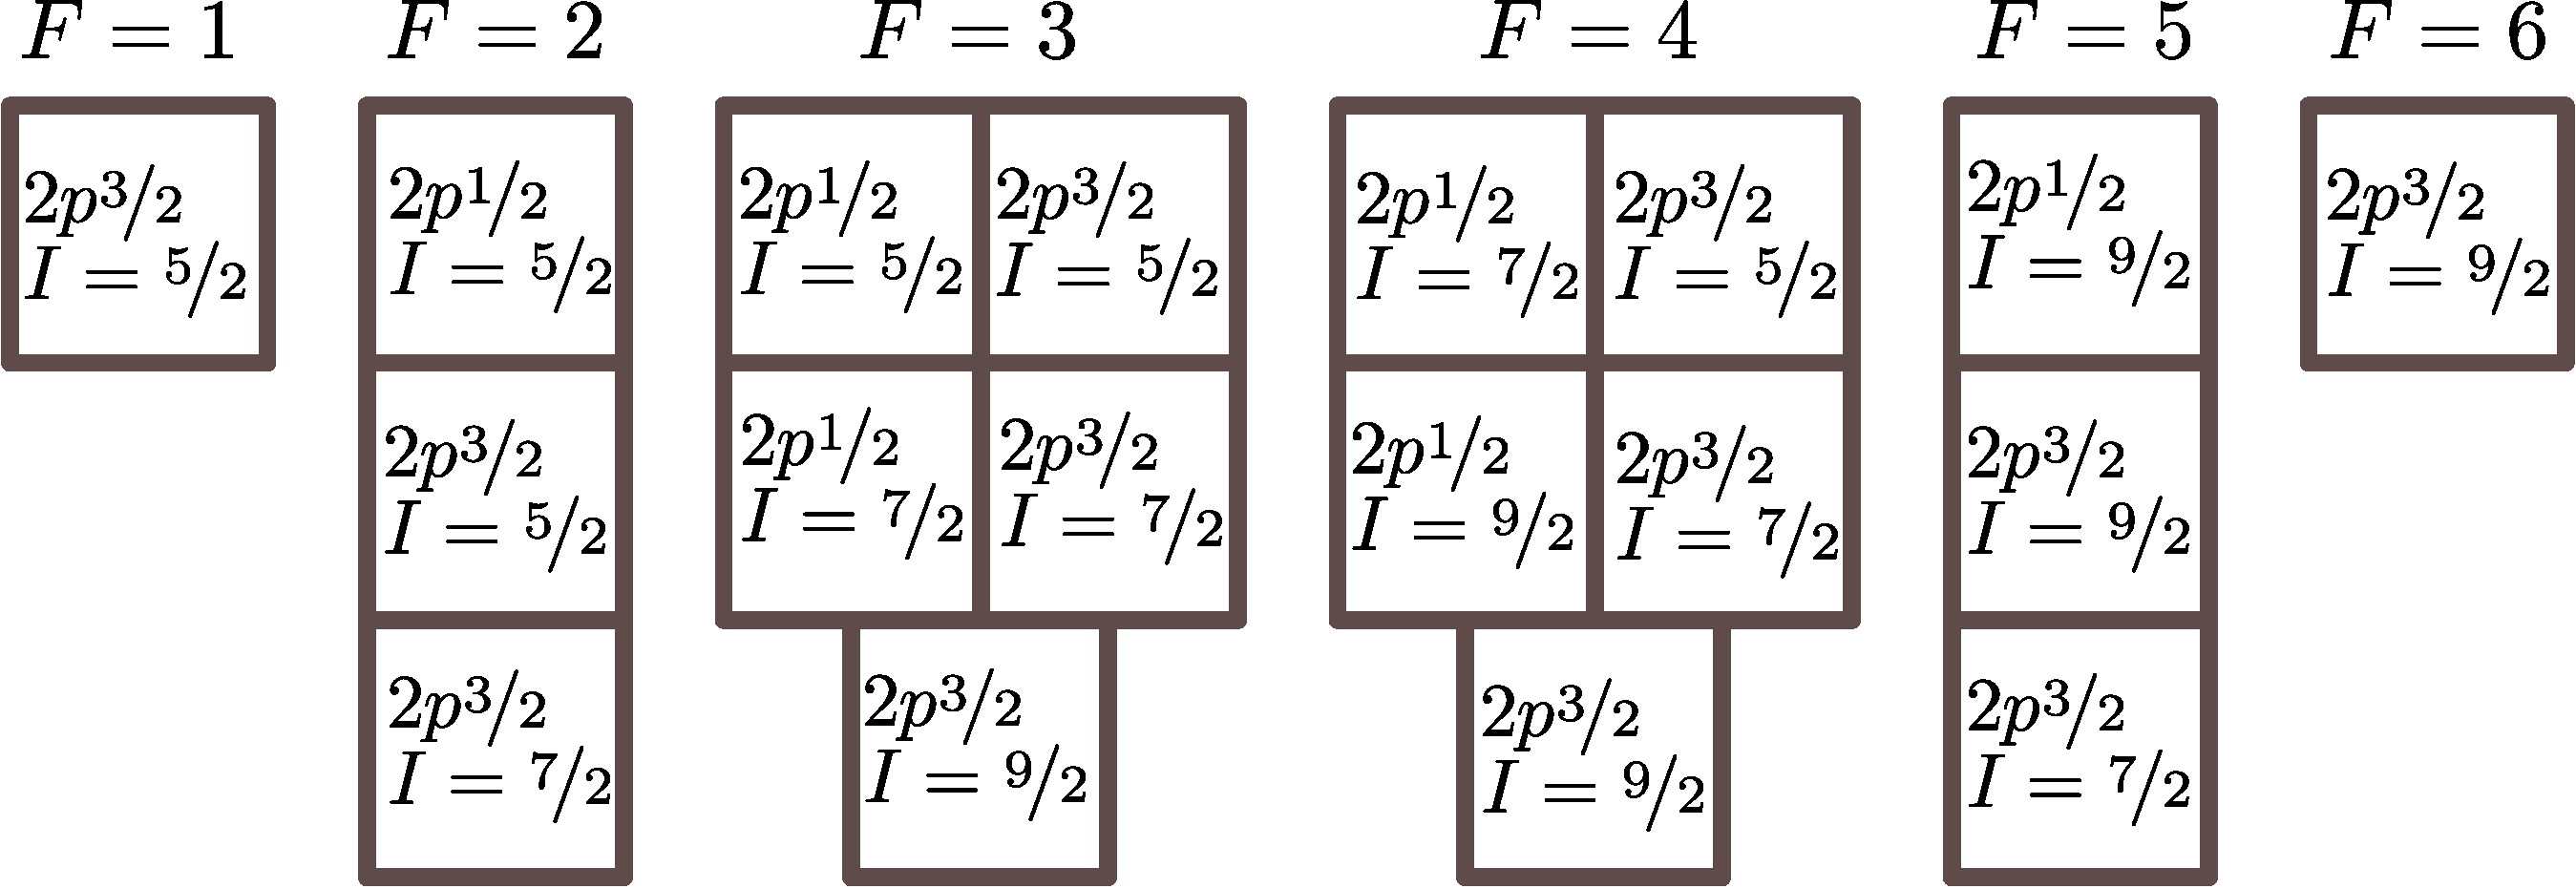
\includegraphics[width=0.91\linewidth]{pics/blocksRe.pdf}%
\caption{Separation of the modelspace consisting of the muonic $2p\nicefrac{1}{2}$ and $2p\nicefrac{3}{2}$ states coupled to the nuclear states with angular momentum $5/2$, $7/2$, and $9/2$. For every possible value of $F\in \{1,...,6\}$, the states are shown, which are involved in the rediagonalization of the hyperfine interaction.}%
\label{fig:blockRe}%
\end{figure}
%
%
\begin{figure}%
\centering
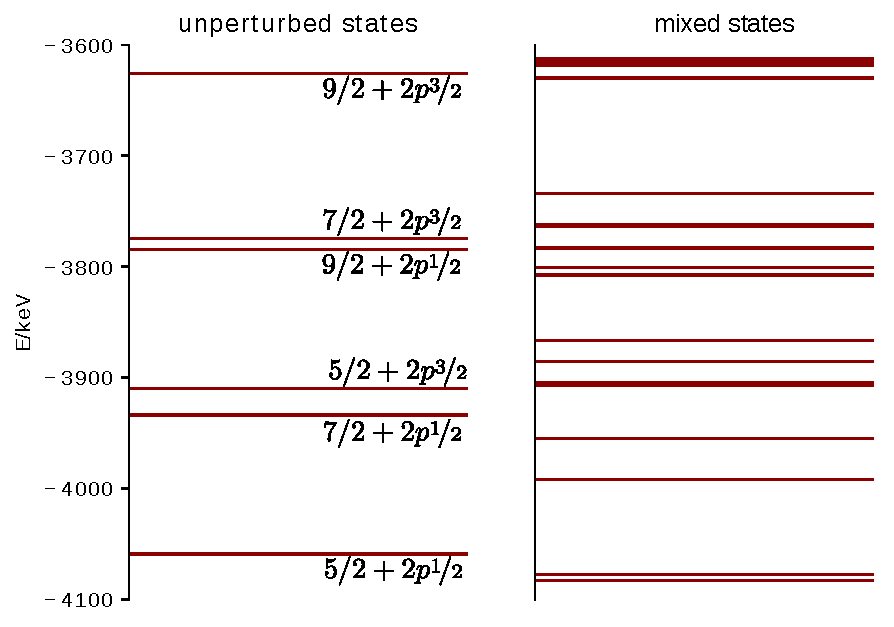
\includegraphics[width=0.88\linewidth]{pics/quad2.pdf}%
\caption{Level scheme of the muonic $2p\nicefrac{1}{2}$ and $2p\nicefrac{3}{2}$ states coupled to the nuclear 5/2, 7/2, and 9/2  states in $^{185}$Re. Zero energy corresponds to the free, resting muon and the nuclear ground state. Through the nuclear rotational states and the strong quadrupole interaction, there is no clear distinction between fine- and hyperfine structure, which results in a rich structure of the energy levels.}%
\label{fig:quad2}%
\end{figure}
%

\subsection{Transition probabilities and intensities}
It has been shown in Sec.~\ref{sec:muon_dynamic} that the coupling of muonic states and nuclear rotational states in connection with a strong quadrupole interaction leads to a rich and complicated level structure without a clear distinction of fine- and hyperfine structure. As a result, there is a large number of potential transitions between the states. For example, if the $L$ x rays are considered, i.e. the transitions from the $3d$ fine structure doublet to the $2p$ fine structure doublet, there are only four transitions if the hyperfine structure is not considered. One of these transitions is suppressed because it is not an electric dipole transition. On the other hand, due to the dynamic hyperfine structure, there are in principle hundreds of $L$ x rays, many of them electric dipole type. As a consequence, for the comparison with experimental spectra, not only the level structure is needed, but also the corresponding relative intensities. Important for the comparison with experiments in the intensity of a transition, which is proportional to the number of measured photons with the energy of the transitions. The intensities are a product of two quantities: Firstly, the intensity is proportional to the transition probability, which can be calculated in principle, as soon as the wave functions and corresponding energies are known. Secondly, the intensities are proportional to the population of the initial state. However, for calculating the population of the initial states, all transition to the initial state from even higher states has to be considered. This eventually leads to a cascade calculation for the muon. Therefore, in the following the transition probabilities and the the population and cascade calculations are discussed separately.

\subsubsection{Transition probabilities}
\label{sec:tranProbs}
In this Section, the transition probabilities due to spontaneous emission of a photon in a muonic transition is analyzed. Starting point is the general formula for the Einstein coefficient (transition probability per time) for state with defined total angular momentum from an initial state $\left|F_iM_i,i_i\right>$ to a final state $\left|F_fM_f,i_f\right>$, where the states are defined in Eq.~\eqref{eq:rediagonState}. Following~\cite[Section 6.]{johnson2007}, this expression reads as
\begin{equation}
\label{eq:transitionGeneral}
A^{(\lambda)}_{J}=\frac{2\alpha (2J+1)(J+1)}{J}\Delta E\,\sum_{M,M_i,M_f} \left|\left<F_fM_f,i_f\middle|\hat{t}^{(\lambda)}_{JM}\middle|F_iM_f,i_i\right>\right|^2,
\end{equation}
where $\Delta E$ is the energy difference of the initial and final state, $J$ is the total angular momentum of the photon and $\lambda=1$ is an electric transition, whereas $\lambda=0$ is a magnetic transition. The multipole transition operator $\hat{t}^{(\lambda)}_{JM}$ is defined in Eqs.~(6.120), (6.121), (6.128),(6.129) of~\cite{johnson2007} in terms of the multipole components of the vectorpotential $\mathbf{a}^{(\lambda)}_{JM}$ and of the scalar potential $\Phi_{JM}$ as
\begin{equation}
\boldsymbol{\alpha}\cdot \mathbf{a}^{(\lambda)}_{JM}(\mathbf{r}_\mu) - \Phi_{JM}(\mathbf{r}_\mu) = i\sqrt{\frac{(2J+1)(J+1)}{4\pi J}}\hat{t}^{(\lambda)}_{JM}(\mathbf{r}_\mu).
\end{equation}
Using the definition of Eq.~\eqref{eq:rediagonState}, the matrix elements are written as
\begin{equation}
\label{eq:tranElement1}
\left<F_fM_f,i_f\middle|\hat{t}^{(\lambda)}_{JM}\middle|F_iM_f,i_i\right> = 
\sum_{k_i,\,k_f}\alpha^{(i_f)\,*}_{k_f} \alpha^{(i_i)}_{k_i}\left<F_fM_f\,I_{k_f}K\,n_{k_f}\kappa_{k_f} \middle|\hat{t}^{(\lambda)}_{JM}\middle|F_iM_i\,I_{k_i}K\,n_{k_i}\kappa_{k_i}\right>.
\end{equation}
Since muonic transitions are considered in this section, it acts on the muonic coordinates $\mathbf{r}_\mu$, which is one subsystem of the composite states in Eq.~\eqref{eq:transitionGeneral} with total angular momentum $F_i$ and $F_f$, respectively. Since the multipole transition operator is an irreducible tensor operator of rank $J$, Eq.~\eqref{app:subsystem_expectation} can be used for calculating the matrix elements. This results in the following expression for the matrix elements:
\begin{alignat}{2}
\left<F_fM_f\,I_{k_f}K\,n_{k_f}\kappa_{k_f} \middle|\hat{t}^{(\lambda)}_{JM}\middle|F_iM_i\,I_{k_i}K\,n_{k_i}\kappa_{k_i}\right>=\delta_{I_{k_f}I_{k_i}}(-1)^{F_i+j(\kappa_{k_f})+I_{k_i}-J}
\notag\\[7.5pt]
\times\sqrt{2F_i+1}\text{C}^{F_fM_f}_{F_iM_i\,JM}
\begin{Bmatrix}
j(\kappa_{k_i})&I_{ki}&F_i\\
F_f&J&j(\kappa_{k_f})
\end{Bmatrix}
\left< n_{k_f}\kappa_{k_f}\middle|\middle|\hat{t}^{(\lambda)}_{J}\middle|\middle|n_{k_i}\kappa_{k_i}\right>
\label{eq:tranElement2}
\end{alignat}
The Clebsch-Gordan coefficients in Eq.~\eqref{eq:tranElement2} do not depend on the summation indices $k_i$ and $k_f$, and the only dependency on the projection numbers $M$, $M_f$, and $M_i$ are as arguments of the Clebsch-Gordan coefficients. Therefore, the summation over $M$, $M_f$, $M_i$ only affacts the Clebsch-Gordan coefficient and the sum rule~\cite{varshalovich1988}
\begin{equation}
\sum_{M,M_i,M_f}\left(C^{F_fM_f}_{F_iM_i\,JM}\right)^2 = 2F_f+1
\end{equation}
can be used to simplify the calculation of Eq.~\eqref{eq:transitionGeneral} considerably. The reduced matrix elements in the muonic variables in Eq.\eqref{eq:tranElement2} can be evaluated in length gauge as~\cite{johnson2007}
\begin{alignat}{2}
&\left< n_{f}\kappa_{f}\middle|\middle|\hat{t}^{(1)}_{J}\middle|\middle|n_{i}\kappa_{i}\right>=&&
\left<n_f\kappa_f\middle|\middle|C_J\middle|\middle|n_i\kappa_i\right>\\
&&&\times\int\text{d}r \text{\huge[}\frac{\kappa_f-\kappa_i}{J+1}\left(j^\prime_J(\Delta E\,r)\right)(G_{n_f\kappa_f}(r)F_{n_i\kappa_i}(r)+G_{n_i\kappa_i}(r)F_{n_f\kappa_f}(r))\\
&&& \hspace{1.5cm}+J\frac{j_J(\Delta E\,r)}{\Delta E\,r}\left(F_{n_f\kappa_f}(r)G_{n_i\kappa_i}(r)-G_{n_f\kappa_f}(r)F_{n_i\kappa_i}(r)\right)\text{\huge]}
\end{alignat}
for electric transitions with $\lambda= 1 $ and as
\begin{alignat}{2}
&\left< n_{f}\kappa_{f}\middle|\middle|\hat{t}^{(0)}_{J}\middle|\middle|n_{i}\kappa_{i}\right>=&&
\left<n_f\,-\kappa_f\middle|\middle|C_J\middle|\middle|n_i\kappa_i\right>\notag\\
&&&\times\int\text{d}r\frac{\kappa_i+\kappa_f}{J+1}j_J(\Delta E\,r)\left(-G_{n_f\kappa_f}(r)F_{n_i\kappa_i}(r)-F_{n_f\kappa_f}(r)G_{n_i\kappa_i}(r)\right)
\end{alignat}
for magnetic transitions with $\lambda = 0$. The reduce matrix elements of the normalized spherical harmonics $\text{C}_{JM}(\vartheta,\varphi)$ read as~\cite{johnson2007}
\begin{equation}
\left<n_f\kappa_f\middle|\middle|C_J\middle|\middle|n_i\kappa_i\right>=(-1)^{j(\kappa_f)+1/2}\sqrt{(2j(\kappa_i)+1)(2j(\kappa_f)+1)}
\begin{pmatrix}
j(\kappa_f)&j(\kappa_i)&J\\
-\nicefrac{1}{2}&\nicefrac{1}{2}&0
\end{pmatrix}
\pi(l(\kappa_f)+l(\kappa_i)+J),
\end{equation}
where the function $\pi(x)$ is defined in Eq.~\eqref{eq:parityFunc}.
\subsubsection{Population of initial states and muonic cascade}
After the transition probabilities have been discussed in Sec.~\ref{sec:tranProbs}, the remaining issue of the initial population is discussed in this Section.
The muonic cascade is visualized in Fig.~\ref{fig:cascade}.
%
\begin{figure}%
\centering
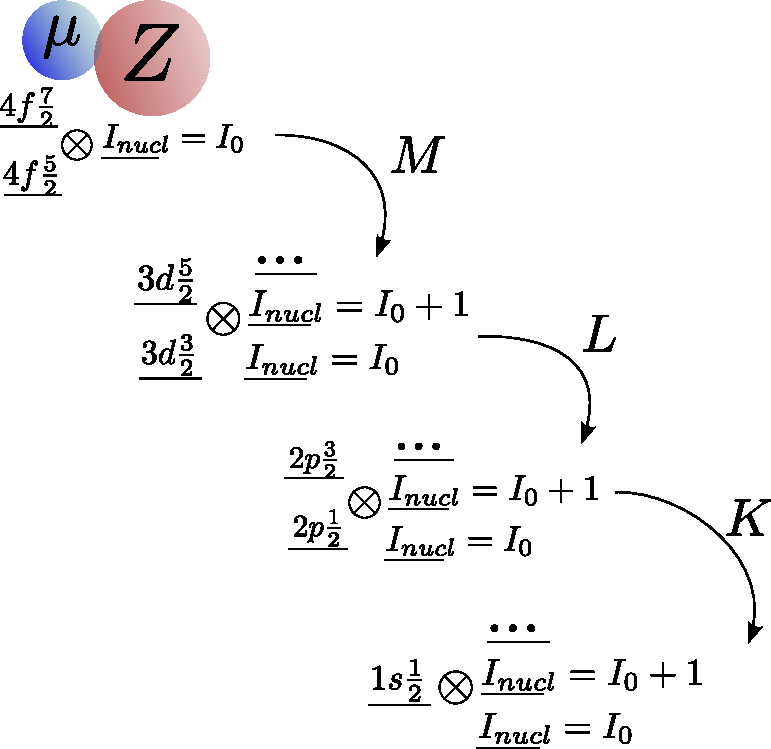
\includegraphics[width=0.62\linewidth]{pics/cascade.pdf}%
\caption{Visualization of the muonic cascade, starting from the muonic $4f$ states and the nucleus in its ground state, Then, the muon is cascading towords its ground state through the $3d$ and $2p$ states. The population of a state in the $3d$ modelspace is obtained by summing up all transitions from the $4f$ states to this state. In this way, all intensities can be calculated starting from a given initial population of the $4f$ states.}%
\label{fig:cascade}%
\end{figure}
%

\section{Higher order corrections for the dynamic hyperfine structure}

\subsection{Residual second order corrections}
\label{sec:muon_residualSO}

\subsection{Quadrupole-Uehling interactions}
\label{sec:muon_quadUehl}

\section{Struture of muonic Rhenium-185}
\label{sec:muon_re}

\subsection{Low lying states}
\subsection{Extraction of quadrupole moment from $5g\rightarrow 4f$ transitions}



\section{Bound muon g factor in Helium-4}
\label{sec:muon_he}

\section{Summary}
\label{sec:muon_summary}
 
  
  %\chapter{Muonic papers}

\begin{itemize}
\item multipole expansion of arbitrary nuclear potential
\item Introduce magnetic dipole and electric quadrupole hyperfine splitting in the Furry picture
\item introduce vacuum polarization corrections (Uehl, Quad-Uehl, WK, KS)
\item Describe usage of modified wave functions (Uehl+WK+KS)
\item Describe g factor correction for bound muon due to Uehl+KS (our PRD)
\item Describe modification of matrix elements with Quad-Uehl
\item Introduce dynamic hyperfine structure
\item Describe calculations of second order terms
\item Description of transition probabilities with hyperfine states
\end{itemize} 


\section{Introduction}
A muon is a charged elementary particle, which is in many aspects similar to the electron, in particular, it has the same electric charge, but it is ${\approx}\,{200}$ times heavier than the electron~\cite{codata}. When coming close to an atom, a muon can be captured by the nucleus and form a hydrogen-like muonic ion, which is typically also surrounded by the atomic electrons. This atomic system is commonly referred to as a muonic atom. The lifetime of the muon is big enough to be considered stable in the structure calculations of these muonic bound states. Muonic atomic systems feature strong dependence on nuclear parameters and therefore can provide information about atomic nuclei \cite{Wheeler1949}. This triggered interest in precise knowledge of the level structure of muonic atoms \cite{BorieRinker1982,Devons1995}. Due to the muon's high mass, it is located much closer to the nucleus; and, especially for heavy nuclei, this results in big nuclear size effects and a strong dependence of the muon bound state energies on the nuclear charge and current distributions, as well as large relativistic effects.

A combination of the knowledge about the level structure and experiments measuring the transition energies in muonic atoms enabled the determination of nuclear parameters like charge radii \cite{Piller1990,Schaller1980}, quadrupole moments \cite{Dey1979}, and magnetic HFS constants \cite{Ruetschi1984}. One of the most precise measurements to date is the determination of the nuclear root-mean-square radius of $^{208}$Pb on a $0.2\%$ level~\cite{Bergem1988}.

Recent measurements on muonic hydrogen renewed the interest in muonic atoms, revealing a disagreement between the values for the proton charge radius extracted from muonic and electronic systems \cite{Pohl2010}. This allows the assumption that there can be unidentified effects in muonic systems, and triggered detailed theoretical investigation of muonic hydrogen und light muonic atoms, e.g., Refs \cite{indelicato2013,pachucki2015}. Deeper knowledge of the physics of heavy muonic atoms could also contribute to the understanding of the muonic puzzles. In addition, nuclear parameters obtained from muonic x rays would be beneficial for experiments on atomic parity violation \cite{Wansbeek2008}. For this reason, there are upcoming experiments on heavy muonic atoms \cite{kirch2016}. The complicated level structure of these systems demands accurate theoretical calculations.

We present updated state-of-the-art calculations of the fine and hyperfine structure of heavy muonic atoms and analyze the individual contributions. In combination with experimental data, they can be used for the determination and further improvement of values of nuclear parameters. The fine structure is calculated including finite size effects and leading order effects of the vacuum polarization. Additionally, the screening from the surrounding atomic electrons is considered. The hyperfine structure is then calculated with extended quadrupole and magnetization distributions, including the previously mentioned effects. Results are presented for muonic $^{205}$Bi, $^{147}$Sm, and $^{89}$Zr. The dual-kinetic-balance method \cite{Shabaev2004} was applied for the numerical evaluation of the listed contributions.

Muonic relativistic units with ${\hbar}{=}{c}{=}{m_\mu}{=}{1}$ are used, where $m_\mu$ is the muon's mass, and the Heavyside charge unit with $\alpha=e^2/4\pi$, where $\alpha$ is the fine structure constant and the electron's charge is ${e}{<}{0}$.
%
%
\section{Interaction between Muon and Nucleus}
The total Hamiltonian for a muon bound to a nucleus can be written as a sum of nuclear, muonic, and interaction Hamiltonian \cite{Devons1995}. Thus, we consider the Hamiltonian
\begin{equation}
H = H_{N} + H^{(0)}_{\mu} + H_{\mu - N},
\end{equation}
with the nuclear Hamiltonian $H_{N}$, the Dirac Hamiltonian $H^{(0)}_{\mu}$ for the free muon, and the interaction Hamiltonian $H_{\mu - N}$. The nucleus is described in the rotational model, i.e. in a state with well defined angular momentum and charge- and current density in the body fixed nuclear frame \cite{kozhedub2008}. As a next step, the interaction between the bound muon and the atomic nucleus is expanded, where electric and magnetic interactions are taken into account. The interaction Hamiltonian is
\begin{equation}
\label{eq:Hint}
H_{\mu - N} = H_{E} + H_{M}
\end{equation}
where the electric part reads
\begin{equation}
\label{eq:elInt}
H_{E}= - \alpha \int \mathrm{d}V^{\prime}\, \frac{\rho (\vec{r}^{\,\prime})}{|\vec{r}_{\mu}-\vec{r}^{\,\prime}|} ,
\end{equation}
with the fine structure constant $\alpha$, the position $\vec{r}^{\,\prime}$ of the nuclear charge distribution and the position $\vec{r}_{\mu}^{\,\prime}$ of the muon in the nuclear frame. The nuclear charge distribution $\rho(\vec{r})$ is normalized to the nuclear charge $Z$ as
\begin{equation}
\label{eq:norm}
\int \mathrm{d}V\rho(\vec{r}) = Z.
\end{equation}
Conveniently, the nuclear charge distribution is divided into a spherically symmetric part $\rho_0(r)$ and a part $\rho_2(r)$ describing the quadrupole distribution in the nuclear frame as \cite{hitlin1970}
\begin{equation}
\label{eq:rho}
\rho(\vec{r}^{\,\prime}) = \rho_0(r^{\prime}) + \rho_2(r^{\prime}) \, Y_{20}(\vartheta^\prime,\varphi^\prime),
\end{equation}
with the spherical harmonics $Y_{lm}(\vartheta,\varphi)$. Since an analogous part for the dipole distribution would be an operator of odd parity, it would vanish after averaging with muon wave functions of defined parity \cite{johnson2007}, and thus it is not considered here and neither are higher multipoles beyond the quadrupole term. Correspondingly, the electric interaction Hamiltonian from (\ref{eq:Hint}) can be written as
\begin{equation}
\label{eq:quadInt}
H_E = H^{(0)}_E + H^{(2)}_E,
\end{equation}
where the spherically symmetric part of the charge distribution gives rise to
\begin{equation}
\label{eq:Hmonopole}
H^{(0)}_E(r_\mu)= - 4 \pi \alpha \int_0^\infty \mathrm{d}r \, r^2 \frac{\rho_0(r)}{r_>},
\end{equation}
with $r_>=\text{max}(r,r_\mu)$. This interaction Hamiltonian will be included in the numerical solution of the Dirac equation for the muon as described in Sec. \ref{sec:radialEq}. The quadrupole part of the interaction $H^{(2)}_E$ causes hyperfine splitting, which is calculated perturbatively in Sec. \ref{sec:elQuad}.\\

As for the magnetic part, we consider dipole interaction. Therefore, the corresponding interaction Hamiltonian from (\ref{eq:Hint}) reads \cite{Elizarov2005}
\begin{equation}
\label{eq:Hmag}
H_{M} = \frac{|e|}{4 \pi}\,\vec{\mu}\cdot \left( F_{\text{BW}}(r) \frac{\vec{r}}{r^3} \times \vec{\alpha} \right),
\end{equation}
with the charge of the muon $e=-|e|$, the nuclear magnetic moment $\vec{\mu}$, its distribution function $F_{\text{BW}}$, and the Dirac matrices $\vec{\alpha}$. If the nuclear current density is described by a normalized scalar function $f_\mu(r)$ as
\begin{equation}
\label{eq:currentdistr}
\vec{j}(r)= \text{rot}\left(\vec{\mu}f_\mu(r)\right),
\end{equation}
then the distribution function is given by
\begin{equation}
\label{eq:Fbw}
F_{\text{BW}}(r)=-r^2 \frac{\partial}{\partial r}\,\int \text{d}V^{\prime}\,\frac{f_\mu(r^{\prime})}{|\vec{r}-\vec{r}\,^{\prime}|}.
\end{equation}
The difference in the hyperfine splitting between a point-like magnetic moment and a spacial distribution of the magnetization is called the Bohr-Weisskopf effect \cite{bohrWeisskopf1950}. In Sec. \ref{sec:elQuad}, the matrix elements of the magnetic interaction are analyzed, paying special attention to the distribution function $F_{\text{BW}}$. We expect the contribution of the higher-order terms, namely electric octupole, magnetic quadrupole, and beyond, to be smaller than the uncertainty of the considered terms \cite{Devons1995,Steffen1985}. Therefore they can be ignored here.

For evaluating these Hamiltonians, the appropriate states are states of defined total angular momentum. A nuclear state $\ket{IM}$ with nuclear angular momentum quantum number $I$ and projection $M$ on the $z$ axis of the laboratory frame and a muonic state $\ket{n\kappa m}$ with total angular momentum $j(\kappa)=|\kappa|-\frac{1}{2}$ and projection $m$ are coupled to a state $\ket{FM_FI\kappa}$ with angular momentum $F$ and projection $M_F$ as
\begin{equation}
\label{eq:totalState}
\ket{FM_FI\kappa}=\sum_{M,m} C^{FM_F}_{IM\,jm} \ket{I M} \, \ket{n\kappa m},
\end{equation}
where $C^{jm}_{j_1m_1j_2m_2}$ are the Clebsch-Gordan coefficients \cite{varshalovich1988}. Here, $n$ is the principal quantum number of the muon and $\kappa=(-1)^{j+l+\frac{1}{2}}(j+\frac{1}{2})$ with the orbital angular momentum quantum number $l$.
%
%
\section{Dirac equation with finite size corrections}
\label{sec:radialEq}
As a basis for further calculations, the Dirac equation
\begin{equation}
\label{eq:diracSph}
\left( \vec{\alpha}\cdot \vec{p}+ \beta + V(r_\mu) \right) \ket{n \kappa m} = (1-E_{n \kappa}) \ket{n \kappa m}
\end{equation} 
is solved for the muon. Here, $\vec{\alpha}$ and $\beta$ are the four Dirac matrices, $E_{n \kappa}$ are the binding energies, and the potential $V(r)$ is the spherically symmetric part of the interaction with the nucleus, which is the monopole contribution from the electric interaction (\ref{eq:Hmonopole}) and the Uehling potential from (\ref{eq:uehl_2}). A Fermi type charge distribution \cite{Beier2000} is used to model the monopole charge distribution as
\begin{equation}
\label{eq:fermi}
\rho_0 (r)=\frac{N}{1+\text{exp}((r-c)/a)},
\end{equation}
where $a$ is a skin thickness parameter and $c$ the half-density radius. The normalization constant $N$ is chosen such that (\ref{eq:norm}) is fulfilled. It has been proven, that $a=t/(4\,\text{log}3)$, with $t=2.30\,\text{fm}$, is a good approximation for most of the nuclei \cite{Beier2000}. The parameter $c$ is then determined by demanding, that the charge radius squared
\begin{equation}
\left<r^2\right>=\cfrac{\int\text{d}r \, r^4\rho_0(r)}{\int\text{d}r \, r^2\rho_0(r)}
\end{equation}
agrees with the values from the literature \cite{Angeli2013}. Since the potential in (\ref{eq:diracSph}) is spherically symmetric, the angular part can be separated and the solution with spherical spinors $\Omega_{\kappa m}(\vartheta,\varphi)$ can be written as \cite{greiner2000}
\begin{equation}
\ket{n\kappa m}=\frac{1}{r}\colvec{2}{G_{n\kappa}(r)\,\Omega_{\kappa m}}{i\,F_{n\kappa}(r)\,\Omega_{-\kappa m}},
\end{equation}
and the resulting equations for the radial functions are solved with the dual-kinetic-balance method \cite{Shabaev2004} to obtain $G_{n\kappa}$ and $F_{n\kappa}$, and the corresponding eigenenergies numerically. 

In Table \ref{tab:sphDirac}, the binding energies for muonic $^{205}_{83}$Bi, $^{147}_{62}$Sm, and $^{89}_{40}$Zr are shown, both with and without the corrections from the Uehling potential (\ref{eq:uehl_2}). The finite nuclear size effect is illustrated by also including the binding energies $E^{(C)}_{n\kappa}$ of the pure Coulomb potential $-Z\alpha / r_\mu$, which read \cite{greiner2000}
\begin{equation}
\label{eq:finestructure_formula_2}
E^{(C)}_{n\kappa}=1-\left(1+\frac{(Z\alpha)^2}{\left( n-|\kappa|+\sqrt{\kappa^2-(Z\alpha)^2} \right)^2}\right)^{-\frac{1}{2}}.
\end{equation}
The uncertainties include the error in the rms radius value as well as a model error, which is estimated via the difference of the binding energies with the Fermi potential (\ref{eq:fermi}) and the potential of a charged sphere with the same rms radius. For heavy nuclei, the finite nuclear size correction can amount up to 50$\,\%$, and thus the binding energy is halved.

%begin table
\begin{table}[b]
\caption{\label{tab:sphDirac}
Overview of the binding energies for muonic $^{205}_{83}$Bi, $^{147}_{62}$Sm, and $^{89}_{40}$Zr, obtained by solving the Dirac equation with the spherically symmetric parts of the muon-nucleus interaction. The values for solving the Dirac equation only with the electric monopole potential, and with the electric monopole potential and the Uehling potential are presented to show the influence of the leading order vacuum polarization. The binding energies (\ref{eq:finestructure_formula_2}) for a  point like nucleus are shown as well. The reduced mass is used to include the non-relativistic recoil corrections from Section \ref{sec:recoil}. The corrections from section \ref{sec:screen} are not included in this table. All energies are in keV.}
%\begin{ruledtabular}
\begin{tabular}{cclll}
& state & \text{point like}& \text{finite size (fs)}\footnotemark[1] &\text{fs+Uehling}\footnotemark[2]\\ \hline \\[-7pt]
$^{205}$Bi & 1s\nicefrac{1}{2} &\text{21573.3} & \text{10699.(51.)} &\text{10767.(52.)} \\
  & 2s\nicefrac{1}{2} & \text{\phantom{1}5538.6} & \text{\phantom{1}3654.(15.)} & \text{\phantom{1}3674.(15.)}\\
  & 2p\nicefrac{1}{2} & \text{\phantom{1}5538.6} & \text{\phantom{1}4893.(3.)} & \text{\phantom{1}4927.(3.)} \\
  & 2p\nicefrac{3}{2} & \text{\phantom{1}4958.9} & \text{\phantom{1}4706.(5.)} & \text{\phantom{1}4737.(5.)} \\
  & 3s\nicefrac{1}{2} & \text{\phantom{1}2394.3} & \text{\phantom{1}1796.(5.)} & \text{\phantom{1}1804.(6.)} \\
  & 3p\nicefrac{1}{2} & \text{\phantom{1}2394.3} & \text{\phantom{1}2170.0(5)} & \text{\phantom{1}2190.1(5)} \\
  & 3p\nicefrac{3}{2} & \text{\phantom{1}2221.4} & \text{\phantom{1}2131.(1.)} & \text{\phantom{1}2141.(1.)} \\
  & 3d\nicefrac{3}{2} & \text{\phantom{1}2221.4} & \text{\phantom{1}2216.9(3)}& \text{\phantom{1}2227.8(3)}\\
  & 3d\nicefrac{5}{2} & \text{\phantom{1}2174.6} & \text{\phantom{1}2172.8(2)} & \text{\phantom{1}2183.0(2)} \\[7pt]
 $^{147}$Sm & 1s\nicefrac{1}{2} & \text{11423.8} & \text{\phantom{1}7165.(28.)} & \text{\phantom{1}7213.(29.)} \\
  & 2s\nicefrac{1}{2} & \text{\phantom{1}2895.7} & \text{\phantom{1}2230.(7.)} & \text{\phantom{1}2242.(7.)} \\
  & 2p\nicefrac{1}{2} & \text{\phantom{1}2895.7} & \text{\phantom{1}2778.(2.)} & \text{\phantom{1}2795.(2.)} \\
  & 2p\nicefrac{3}{2} & \text{\phantom{1}2736.9} & \text{\phantom{1}2689.(2.)} & \text{\phantom{1}2706.(2.)} \\
  & 3s\nicefrac{1}{2} & \text{\phantom{1}1268.9} & \text{\phantom{1}1061.(2.)} & \text{\phantom{1}1066.(2.)} \\
  & 3p\nicefrac{1}{2} & \text{\phantom{1}1268.9} & \text{\phantom{1}1228.6(4)} & \text{\phantom{1}1234.2(4)} \\
  & 3p\nicefrac{3}{2} & \text{\phantom{1}1221.7} & \text{\phantom{1}1204.7(6)} & \text{\phantom{1}1210.0(6)} \\
  & 3d\nicefrac{3}{2} & \text{\phantom{1}1221.7} & \text{\phantom{1}1221.4(1)} & \text{\phantom{1}1226.2(1)} \\
  & 3d\nicefrac{5}{2} & \text{\phantom{1}1207.6} & \text{\phantom{1}1207.4} & \text{\phantom{1}1212.1} \\[7pt]
 $^{89}$Zr & 1s\nicefrac{1}{2} & \text{\phantom{1}4595.5} & \text{\phantom{1}3643.(8.)} & \text{\phantom{1}3669.(8.)} \\
  & 2s\nicefrac{1}{2} & \text{\phantom{1}1155.2} & \text{\phantom{1}1021.(2.)} & \text{\phantom{1}1026.(2.)} \\
  & 2p\nicefrac{1}{2} & \text{\phantom{1}1155.2} & \text{\phantom{1}1147.8(2)} & \text{\phantom{1}1153.7(2)} \\
  & 2p\nicefrac{3}{2} & \text{\phantom{1}1129.9} & \text{\phantom{1}1127.0(2)} & \text{\phantom{1}1132.6(2)} \\
  & 3s\nicefrac{1}{2} & \text{\phantom{11}510.6} & \text{\phantom{11}469.8(5)} & \text{\phantom{11}471.4(5)} \\
  & 3p\nicefrac{1}{2} & \text{\phantom{11}510.6} & \text{\phantom{11}508.0(1)} & \text{\phantom{11}509.8(1)} \\
  & 3p\nicefrac{3}{2} & \text{\phantom{11}503.1} & \text{\phantom{11}502.0(1)} & \text{\phantom{11}503.8(1)} \\
  & 3d\nicefrac{3}{2} & \text{\phantom{11}503.1} & \text{\phantom{11}503.1} & \text{\phantom{11}504.5} \\
  & 3d\nicefrac{5}{2} & \text{\phantom{11}500.7} & \text{\phantom{11}500.7} & \text{\phantom{11}502.1} \\

\end{tabular}
%\end{ruledtabular}
\footnotetext[1]{$V(r_\mu)=H^{(0)}_E(r_\mu)$}
\footnotetext[2]{$V(r_\mu)=H^{(0)}_E(r_\mu)+V_{\text{Uehl}}(r_\mu)$
%\footnotetext[3]{$V(r_\mu)=-Z\alpha/r_\mu$
\\see eq. (\ref{eq:Hmonopole}), (\ref{eq:diracSph}), and (\ref{eq:uehl_2}) for definitions}
\end{table}
%end table
%
%
\section{Vacuum polarization}
\label{sec:qed}

For atomic electrons, usually the self-energy QED correction is comparable to the vacuum polarization correction \cite{Beier2000}. For muons, however, the vacuum polarization correction is much larger due to virtual electron-positron pairs, which are less suppressed due to their low mass compared to the muon's mass \cite{BorieRinker1982}. The spherically symmetric part of the vacuum polarization to first order in $\alpha$ and $Z\alpha$ is the Uehling potential \cite{Elizarov2005}
\begin{align}
V_{\text{Uehl}}(r_\mu)=-\alpha \frac{2\alpha}{3\pi}\int_0^\infty \text{d}r^{\prime}\,4\pi \rho_0(r^\prime)\int_1^\infty \text{d}t\,\left( 1+\frac{1}{2t^2} \right)\nonumber\\
\times\frac{\sqrt{t^2-1}}{t^2} \frac{\text{exp}(-2m_e|r_\mu-r^\prime|t)-\text{exp}(-2m_e(r_\mu+r^\prime)t)}{4m_er_\mu t},
\label{eq:uehl_2}
\end{align}
where $m_e$ is the electron mass and $\rho_0$ is the spherically symmetric part of the charge distribution from (\ref{eq:rho}). This potential can be directly added to the Dirac equation (\ref{eq:diracSph}). In this way, all iterations of the Uehling potential are included \cite{indelicato2013}. Results for our calculations can be found in Table \ref{tab:sphDirac}.
%
%
\section{Recoil corrections}
\label{sec:recoil}
Taking into account the finite mass and the resulting motion of the nucleus leads to recoil corrections to the bound muon energy levels. In nonrelativistic quantum mechanics, as in classical mechanics, the problem of describing two interacting particles can be reduced to a one particle problem by using the reduced mass $m_r$ of the muon-nucleus system \cite{landaulifshitz3}. With the mass of the nucleus $m_N$, the reduced mass reads in the chosen system of units as
\begin{equation}
\label{eq:redmass}
m_r=\frac{m_N}{m_N+1},
\end{equation}
and the Dirac equation is accordingly modified to
\begin{equation}
\label{eq:diracSphRed}
\left( \vec{\alpha}\cdot \vec{p}+ \beta\,m_r + V(r_\mu) \right) \ket{n \kappa m} = (m_r-E_{n \kappa}) \ket{n \kappa m}.
\end{equation} 
In relativistic quantum mechanics, this separation is not possible. We follow an approach used in Refs. \cite{friar1973,BorieRinker1982}, which includes the nonrelativistic part of the recoil correction already in the wave functions by using the reduced mass in the Dirac equation and calculating the leading relativistic corrections perturbatively. If $E^{\text{(fm)}}_{n\kappa}$ denotes the binding energy of (\ref{eq:diracSph}) with the finite size potential (\ref{eq:Hmonopole}) but with the reduced mass replaced by the full muon rest mass, and $E^{\text{(rm)}}_{n\kappa}$ the binding energy in the same potential but with the reduced mass (\ref{eq:redmass}), then the leading relativistic recoil correction $\Delta E^{\text{(rec,rel)}}_{n\kappa}$ according to Ref. \cite{BorieRinker1982} reads
\begin{equation}
\label{eq:relrec}
\Delta E^{\text{(rec,rel)}}_{n\kappa} = -\frac{\left(E^{\text{(fm)}}_{n\kappa}\right)^2}{2 M_N}+\frac{1}{2 M_N}\left< h(r) + 2 E^{\text{(fm)}}_{n\kappa} P_1(r)  \right>,
\end{equation}
where $M_N$ is the mass of the nucleus, and the functions $h(r)$ and $P_1(r)$ are defined in Eqs. (109) and (111) of Ref. \cite{BorieRinker1982}, respectively. In Table \ref{tab:recoil}, the binding energies obtained from solving the Dirac equation with the muon rest mass and the reduced mass of the muon-nucleus system are compared, and the leading relativistic recoil correction is shown. The uncertainties include errors in the rms radius, the model of the charge distribution and for the relativistic recoil, and a $(m_\mu/M_N)^2$ term due to higher-order corrections in the mass ratio of muon and nucleus, which dominates the uncertainty for lower $Z$.
%begin table
\begin{table}
\caption{\label{tab:recoil}Recoil corrections to the binding energies of the muon. fm (full mass) denotes the finite size binding energy, analogous to the fourth column of Table \ref{tab:sphDirac}, but with the rest mass of the muon used in the Dirac equation. $\Delta E_{\text{rec,nr}}$ is the non-relativistic recoil correction, which is the difference between the finite size Dirac solutions with reduced mass and full mass, respectively. $\Delta E^{\text{(rec,rel)}}_{n\kappa}$ is the leading relativistic recoil correction from Section \ref{sec:recoil}.
All energies are in keV.}
%\begin{ruledtabular}
\begin{tabular}{lllll}
& state & $E^{\text{(fm)}}$ &$\Delta E^{\text{rec,nr}}$&$\Delta E^{\text{(rec,rel)}}_{n\kappa}$\footnotemark[1]\\ \hline \\[-7pt]
 $^{205}$Bi & 1s\nicefrac{1}{2} & \text{10702.(51.)} & \text{-2.80(4)} & \text{0.39(4)} \\
  & 2s\nicefrac{1}{2} & \text{\phantom{1}3656.(15.)} & \text{-1.42(2)} & \text{0.09(3)}\\
  & 2p\nicefrac{1}{2} & \text{\phantom{1}4895.6(3.0)} & \text{-2.24(1)} & \text{0.12(3)} \\
  & 2p\nicefrac{3}{2} & \text{\phantom{1}4708.2(4.6)} & \text{-2.27(1)} & \text{0.01(1)} \\
  & 3s\nicefrac{1}{2} & \text{\phantom{1}1796.6(5.5)} & \text{-0.78(1)} & \text{0.03(3)} \\
  & 3p\nicefrac{1}{2} & \text{\phantom{1}2180.0(0.5)} & \text{-1.05} & \text{0.03(3)} \\
  & 3p\nicefrac{3}{2} & \text{\phantom{1}2131.9(1.3)} & \text{-1.06} & \text{0.03(3)} \\
  & 3d\nicefrac{3}{2} & \text{\phantom{1}2218.1(0.3)} & \text{-1.21} & \text{0.02(2)} \\
  & 3d\nicefrac{5}{2} & \text{\phantom{1}2174.0(0.2)} & \text{-1.19} & \text{0.02(2)} \\[7pt]
 $^{147}$Sm & 1s\nicefrac{1}{2} & \text{\phantom{1}7168.(28.)} & \text{-3.17(4)} & \text{0.29(7)} \\
  & 2s\nicefrac{1}{2} & \text{\phantom{1}2231.1(6.7)} & \text{-1.31(1)} & \text{0.05(5)} \\
  & 2p\nicefrac{1}{2} & \text{\phantom{1}2779.4(1.5)} & \text{-1.97(1)} & \text{0.05(5)} \\
  & 2p\nicefrac{3}{2} & \text{\phantom{1}2691.2(1.8)} & \text{-1.96(1)} & \text{0.04(4)} \\
  & 3s\nicefrac{1}{2} & \text{\phantom{1}1062.0(2.3)} & \text{-0.68(1)} & \text{0.02(2)} \\
  & 3p\nicefrac{1}{2} & \text{\phantom{1}1229.5(0.4)} & \text{-0.89} & \text{0.01(1)} \\
  & 3p\nicefrac{3}{2} & \text{\phantom{1}1205.6(0.6)} & \text{-0.89} & \text{0.01(1)} \\
  & 3d\nicefrac{3}{2} & \text{\phantom{1}1222.3(0.1)} & \text{-0.93} & \text{0.01(1)} \\
  & 3d\nicefrac{5}{2} & \text{\phantom{1}1208.3} & \text{-0.92} & \text{0.01(1)} \\[7pt]
 $^{89}$Zr & 1s\nicefrac{1}{2} & \text{\phantom{1}3646.5(8.2)} & \text{-3.36(3)} & \text{0.15(15)} \\
  & 2s\nicefrac{1}{2} & \text{\phantom{1}1022.4(1.5)} & \text{-1.11(1)} & \text{0.02(2)} \\
  & 2p\nicefrac{1}{2} & \text{\phantom{1}1149.2(0.2)} & \text{-1.43} & \text{0.01(1)} \\
  & 2p\nicefrac{3}{2} & \text{\phantom{1}1128.4(0.2)} & \text{-1.41} & \text{0.01(1)} \\
  & 3s\nicefrac{1}{2} & \text{\phantom{11}470.3(0.5)} & \text{-0.54} & \text{0.01(1)} \\
  & 3p\nicefrac{1}{2} & \text{\phantom{11}508.6(0.1)} & \text{-0.64} & \text{0.00} \\
  & 3p\nicefrac{3}{2} & \text{\phantom{11}502.7(0.1)} & \text{-0.63} & \text{0.00} \\
  & 3d\nicefrac{3}{2} & \text{\phantom{11}503.7} & \text{-0.64} & \text{0.00} \\
  & 3d\nicefrac{5}{2} & \text{\phantom{11}501.3} & \text{-0.63} & \text{0.00} \\
\end{tabular}
%\end{ruledtabular}
\footnotetext[1]{$\Delta E^{\text{rec,nr}}:=E^{\text{(red.mass)}}-E^{\text{(fm)}}$, see Section \ref{sec:recoil} for definitions.}
\end{table}
%end table
%
%
\section{Electron screening}
\label{sec:screen}
%begin table
\begin{table}
\caption{\label{tab:screen}Electron screening corrections to the bound muon energy levels. $\Delta E_{\rm{S,eff}}^{(1)}$ and $\Delta E_{\rm{S,eff}}^{(1+2)}$ are the screening corrections with the effective nuclear charge method, whereas $\Delta E_{\rm{S,3step}}^{(1)}$ and $\Delta E_{\rm{S,3step}}^{(1+2)}$ use the 3 step calculation, both described in Section \ref{sec:screen}. For the superscript $(1)$, only the 1s electrons are considered, while for $({1}{+}{2})$, all electrons from the first and second shell are considered. All energies are in keV.}
%\begin{ruledtabular}
\begin{tabular}{ccrrrr}
&$\mu$-state & $\Delta E_{\rm{S,eff}}^{(1)}$  & $\Delta E_{\rm{S,eff}}^{(1+2)}$ & $\Delta E_{\rm{S,3step}}^{(1)}$ & $\Delta E_{\rm{S,3step}}^{(1+2)}$\\ \hline \\[-7pt]
 $^{205}$Bi & 1s\nicefrac{1}{2} & \text{5.555} & \text{10.825} & \text{5.555} & \text{10.825} \\
  & 2s\nicefrac{1}{2} & \text{5.537} & \text{10.803} & \text{5.538} & \text{10.805} \\
  & 2p\nicefrac{1}{2} & \text{5.548} & \text{10.817} & \text{5.549} & \text{10.818} \\
  & 2p\nicefrac{3}{2} & \text{5.547} & \text{10.816} & \text{5.548} & \text{10.817} \\
  & 3s\nicefrac{1}{2} & \text{5.490} & \text{10.748} & \text{5.494} & \text{10.753} \\
  & 3p\nicefrac{1}{2} & \text{5.514} & \text{10.776} & \text{5.516} & \text{10.779} \\
  & 3p\nicefrac{3}{2} & \text{5.512} & \text{10.774} & \text{5.515} & \text{10.777} \\
  & 3d\nicefrac{3}{2} & \text{5.526} & \text{10.791} & \text{5.528} & \text{10.793} \\
  & 3d\nicefrac{5}{2} & \text{5.525} & \text{10.789} & \text{5.527} & \text{10.792} \\[7pt]
 $^{147}$Sm & 1s\nicefrac{1}{2} & \text{3.705} & \text{7.312} & \text{3.705} & \text{7.312} \\
  & 2s\nicefrac{1}{2} & \text{3.699} & \text{7.305} & \text{3.700} & \text{7.305} \\
  & 2p\nicefrac{1}{2} & \text{3.703} & \text{7.309} & \text{3.703} & \text{7.309} \\
  & 2p\nicefrac{3}{2} & \text{3.703} & \text{7.309} & \text{3.703} & \text{7.309} \\
  & 3s\nicefrac{1}{2} & \text{3.682} & \text{7.285} & \text{3.683} & \text{7.286} \\
  & 3p\nicefrac{1}{2} & \text{3.689} & \text{7.293} & \text{3.691} & \text{7.295} \\
  & 3p\nicefrac{3}{2} & \text{3.689} & \text{7.293} & \text{3.690} & \text{7.294} \\
  & 3d\nicefrac{3}{2} & \text{3.694} & \text{7.299} & \text{3.695} & \text{7.300} \\
  & 3d\nicefrac{5}{2} & \text{3.694} & \text{7.298} & \text{3.694} & \text{7.299} \\[7pt]
 $^{89}$Zr & 1s\nicefrac{1}{2} & \text{2.214} & \text{4.405} & \text{2.214} & \text{4.405} \\
  & 2s\nicefrac{1}{2} & \text{2.212} & \text{4.402} & \text{2.212} & \text{4.403} \\
  & 2p\nicefrac{1}{2} & \text{2.213} & \text{4.403} & \text{2.213} & \text{4.403} \\
  & 2p\nicefrac{3}{2} & \text{2.213} & \text{4.403} & \text{2.213} & \text{4.403} \\
  & 3s\nicefrac{1}{2} & \text{2.205} & \text{4.395} & \text{2.206} & \text{4.396} \\
  & 3p\nicefrac{1}{2} & \text{2.207} & \text{4.397} & \text{2.208} & \text{4.398} \\
  & 3p\nicefrac{3}{2} & \text{2.207} & \text{4.397} & \text{2.208} & \text{4.398} \\
  & 3d\nicefrac{3}{2} & \text{2.209} & \text{4.399} & \text{2.210} & \text{4.400} \\
  & 3d\nicefrac{5}{2} & \text{2.209} & \text{4.399} & \text{2.209} & \text{4.400} \\

\end{tabular}
%\end{ruledtabular}
\end{table}
%end table
The effect of the surrounding electrons on the binding energies of the muon was estimated following Ref. \cite{vogel1973} by calculating an effective screening potential from the charge distribution of the electrons as
\begin{equation}
\label{eq:screenPot}
V_{e}(\vec{r}_\mu)=-\alpha \int \mathrm{d}V\frac{\rho_e (\vec{r})}{|\vec{r}_\mu-\vec{r}|},
\end{equation}
and using this potential in the Dirac equation for the muon. The charge distribution of the electrons is obtained by their Dirac wave functions as $\rho_e (\vec{r})=\sum_i \psi_{e_i}^*(\vec{r})\cdot \psi_{e_i}(\vec{r})$, where $\psi_{e_i}(\vec{r})$  is the four component spinor of the $i$-th considered electron. In order to obtain the wave functions of the electrons, it has to be taken into account, that the muon essentially screens one unit of charge from the nucleus. The simplest possibility is to replace the nuclear charge by an effective charge $\tilde{Z}=Z-1$ and then solve the Dirac equation for the electron with this modified nuclear potential. Another possibility is to start solving the Dirac equation for the muon in the nuclear potential without electron screening. Then, the Dirac equation for the electron is solved for all required states, adding the screening potential due to the bound muon
\begin{equation}
V_{\mu}(\vec{r}_e)=-\alpha \int \mathrm{d}V\frac{\psi_\mu^*(\vec{r})\cdot \psi_\mu(\vec{r})}{|\vec{r}_e-\vec{r}|},
\end{equation}
analogously to (\ref{eq:screenPot}).
The interaction between the electrons is not taken into account here. Finally, the Dirac equation for the muon is solved again, now including the nuclear potential and the screening potential (\ref{eq:screenPot}) due the atomic electrons from the considered electron configuration. This procedure can be repeated in the spirit of Hartree's method \cite{bethe_salpeter} until the electrons and the muon are self-consistent in the fields of each other, but our studies show that one iteration is usually enough since the overlap of muon and electron wave functions in heavy muonic atoms is small. It is important to note, that here the screening potential depends to a small extent on the state of the muon, since the muon wave function is used in the calculation for the electron wave function. The atomic electrons primarily behave like a charged shell around the muon and the nucleus; thus every muon level is mainly shifted by a constant term, which is not observable in muonic transitions. The screening correction $\Delta E_S$ is defined as the difference of the binding energy without screening potential and with screening potential, therefore a positive value indicates that the muon is less bound due to the screening effect. The main contribution to the nonconstant part of the screening potential comes from the 1$s$ electrons, since their wave functions have the biggest overlap with the muon; therefore the exact electron configuration has only a minor effect on transition energies \cite{vogel1973}. In Table \ref{tab:screen}, results for the screening correction are shown for both mentioned methods and for different electron configurations. Values of the screening correction for different electron configurations show that a 10\% error for the non-constant part is a reasonable estimate.
%
%
\section{Hyperfine interactions}
\label{sec:hfs}
\subsection{Electric quadrupole splitting}
\label{sec:elQuad}
%begin hfs table
\begin{table*}
\caption{\label{tab:hfs}
Results for the electric quadrupole and magnetic dipole hyperfine splitting for a selection of hyperfine states of muonic $^{205}_{83}$Bi ($I=\frac{9}{2}$), $^{147}_{62}$Sm ($I=\frac{7}{2}$), and $^{89}_{40}$Zr ($I=\frac{9}{2}$). $\braket{H_E^{(2)}}$ are the values of the electric quadrupole splitting. $\braket{H_M^{\rm{hom}}}$ is the magnetic dipole splitting from (\ref{eq:hmag}) using a homogeneous nuclear current distribution and $\braket{H_M^{\rm{sp}}}$ using the nuclear magnetization distribution in the single particle model. See Section \ref{sec:hfs} for definitions. All energies are in keV.}
%\begin{ruledtabular}
\begin{tabular}{ccllllll}
 nucleus&state&\multicolumn{2}{c}{$\braket{H_E^{(2)}}$}&\multicolumn{2}{c}{$\braket{H_M^{\rm{hom}}}$}&\multicolumn{2}{c}{$\braket{H_M^{\rm{sp}}}$}\\
 & &$F=I-\frac{1}{2}$&$F=I+\frac{1}{2}$&$F=I-\frac{1}{2}$&$F=I+\frac{1}{2}$&$F=I-\frac{1}{2}$&$F=I+\frac{1}{2}$\\[2pt] \hline \\[-7pt]
   $^{205}$Bi & 1s\nicefrac{1}{2} & \phantom{-11}0 & \phantom{-11}0 & -2.27(20) &\phantom{-}1.86(16) & -2.41(20) &\phantom{-}1.97(16) \\
  & 2s\nicefrac{1}{2} & \phantom{-11}0 & \phantom{-11}0 & \text{-0.43(5)} &\phantom{-}0.35(4) & -0.47(6) &\phantom{-}0.38(4) \\
  & 2p\nicefrac{1}{2} & \phantom{-11}0 & \phantom{-11}0 & -1.23(11) & \phantom{-}1.01(9) & -1.31(11) &\phantom{-}1.07(10) \\
  & 2p\nicefrac{3}{2} & -175.(24.) & \phantom{-}175.(24.) & -0.55(2) & \phantom{-}0.010(4) & -0.554(22) & \phantom{-}0.098(4) \\
  & 3s\nicefrac{1}{2} & \phantom{-11}0 & \phantom{-11}0 & \text{-0.144(20)} & \phantom{-}0.118(16) & -0.160(20) & \phantom{-}0.131(16) \\
  & 3p\nicefrac{1}{2} & \phantom{-11}0 & \phantom{-11}0 & -0.311(33) & \phantom{-}0.255(26) & -0.336(33) & \phantom{-}0.275(27) \\
  & 3p\nicefrac{3}{2} & \phantom{1}-48.9(8.0) & \phantom{-1}48.9(8.0) & -0.160(7) & \phantom{-}0.028(1) & -0.163(7) & \phantom{-}0.029(1) \\
  & 3d\nicefrac{3}{2} & \phantom{1}-25.4(1.3) & \phantom{-1}25.4(1.3) & -0.161(6) & \phantom{-}0.028(1) & -0.163(6) & \phantom{-}0.029(1) \\
  & 3d\nicefrac{5}{2} & \phantom{-1}28.3(1.3) & \phantom{1}-28.3(1.3) & -0.103(3) & -0.027 & -0.103(3) & -0.027 \\[7pt]
  $^{147}$Sm & 1s\nicefrac{1}{2} & \phantom{-11}0 & \phantom{-11}0 & \text{\phantom{-}0.42(18)} & -0.33(14) & \phantom{-}0.25(17) & -0.20(14) \\
  & 2s\nicefrac{1}{2} & \phantom{-11}0 & \phantom{-11}0 & \phantom{-}0.072(39) & -0.056(30) & \phantom{-}0.033(39) & -0.026(30) \\
  & 2p\nicefrac{1}{2} & \phantom{-11}0 & \phantom{-11}0 & \phantom{-}0.164(58) & -0.127(45) & \phantom{-}0.106(58) & -0.082(45) \\
  & 2p\nicefrac{3}{2} & \phantom{1}-32.8(3.2) & \phantom{-1}32.8(3.2) & \phantom{-}0.066(8) & -0.004(1) & \phantom{-}0.058(8) & -0.004(1) \\
  & 3s\nicefrac{1}{2} & \phantom{-11}0 & \phantom{-11}0 & \phantom{-}0.023(13) & -0.018(10) & \phantom{-}0.010(13) & -0.008(8) \\
  & 3p\nicefrac{1}{2} & \phantom{-11}0 & \phantom{-11}0 & \phantom{-}0.044(18) & -0.034(14) & \phantom{-}0.026(18) & -0.02(1) \\
  & 3p\nicefrac{3}{2} & \phantom{11}-9.4(1.1) & \phantom{-11}9.4(1.1) & \phantom{-}0.020(3) & -0.001 & \phantom{-}0.017(3) & -0.001 \\
  & 3d\nicefrac{3}{2} & \phantom{11}-3.2(0.1) & \phantom{-11}3.2(0.1) & \phantom{-}0.015(1) & \phantom{-}0.000 & \phantom{-}0.014(1) & \phantom{-}0.000 \\
  & 3d\nicefrac{5}{2} & \phantom{-11}3.7(0.2) & \phantom{11}-3.7(0.2) & \phantom{-}0.010 & \phantom{-}0.004 & \phantom{-}0.010 & \phantom{-}0.004 \\[7pt]
 $^{89}$Zr & 1s\nicefrac{1}{2} & \phantom{-11}0 & \phantom{-11}0 & \phantom{-}0.36(13) & -0.29(10) & \phantom{-}0.23(12) & -0.19(10) \\
  & 2s\nicefrac{1}{2} & \phantom{-11}0 & \phantom{-11}0 & \phantom{-}0.053(23) & -0.043(18) & \phantom{-}0.030(23) & -0.025(18) \\
  & 2p\nicefrac{1}{2} & \phantom{-11}0 & \phantom{-11}0 & \phantom{-}0.071(14) & -0.058(11) & \phantom{-}0.057(14) & -0.047(11) \\
  & 2p\nicefrac{3}{2} & \phantom{-1}12.2(4.7) &\phantom{1}-12.2(4.7) & \phantom{-}0.023(1) & -0.004 & \phantom{-}0.022(1) &-0.004 \\
  & 3s\nicefrac{1}{2} & \phantom{-11}0 & \phantom{-11}0 & \phantom{-}0.016(7) & -0.013(6) & \phantom{-}0.009(7) & -0.007(6) \\
  & 3p\nicefrac{1}{2} & \phantom{-11}0 & \phantom{-11}0 & \phantom{-}0.020(4) & -0.017(4) & \phantom{-}0.016(4) & -0.013(4) \\
  & 3p\nicefrac{3}{2} & \phantom{-11}3.6(1.4) & \phantom{11}-3.6(1.4) & \phantom{-}0.007 & -0.001 & \phantom{-}0.007 & -0.001 \\
  & 3d\nicefrac{3}{2} & \text{\phantom{-11}0.9(0.3)} & \text{\phantom{11}-0.9(0.3)} & \phantom{-}0.004 & \phantom{-}0.000 & \phantom{-}0.004 & \phantom{-}0.000 \\
  & 3d\nicefrac{5}{2} & \text{\phantom{11}-1.1(0.4)} & \text{\phantom{-11}1.1(0.4)} & \phantom{-}0.003 & \phantom{-}0.000 & \phantom{-}0.003 &\phantom{-}0.000 \\

\end{tabular}
%\end{ruledtabular}
\end{table*}
% end hfs table
Since for heavy nuclei the nuclear radius is comparable to the muon's Compton wavelength \cite{Angeli2013,codata}, the muonic wavefunction overlaps strongly with the nucleus and the muon is sensitive to nuclear shape corrections, which results in hyperfine splitting of the energy levels. The quadrupole part of the electric interaction (\ref{eq:quadInt}) can be rewritten as \cite{kozhedub2008}
\begin{equation}
\label{eq:Hquad}
H^{(2)}_E = - \alpha \frac{Q_0 F_{\text{QD}}(r_\mu)}{2\, r_\mu^3} \sum_{m=-2}^2 C_{2m}(\vartheta_N,\varphi_N)C_{2m}^{*}(\vartheta_\mu,\varphi_\mu),
\end{equation}
where $C_{lm}(\vartheta,\varphi)=\sqrt{4\pi/(2l+1)}Y_{lm}(\vartheta,\varphi)$ and angles with a subscript $\mu$($N$) describe the position of the muon ($z$ axis of the nuclear frame) in the laboratory frame. Here, the nuclear intrinsic quadrupole moment is defined via the charge distribution (\ref{eq:rho}) as
\begin{equation}
\label{eq:defQ0}
Q_0 = 2 \sqrt{\frac{4\pi}{5}} \int_0^\infty r^4 \rho_2(r)\,\mathrm{d}r,
\end{equation}
and the distribution of the quadrupole moment is described by the function $f(r_\mu)$, where in the point-like limit $f(r_\mu)=1/r_\mu^{-3}$. For the shell model, where the quadrupole distribution is concentrated around the nuclear rms radius $R_N$, the divergence for $r_\mu=0$ is removed, and the corresponding quadrupole distribution function is
\begin{equation}
F_{\text{QD}}(r_\mu)=
\begin{cases}
\left(\nicefrac{r_\mu}{R_N}\right)^5 & r_\mu \leq R_N\\
1 &r_\mu > R_N
\end{cases}.
\end{equation}
Formally, this corresponds to a charge distribution with
\begin{equation}
\rho_2(r_\mu)=\frac{Q_0}{2 R_N^4}\sqrt{\frac{5}{4\pi}}\delta(r_\mu-R_N).
\end{equation}
The matrix elements of the quadrupole interaction (\ref{eq:Hquad}) in the states (\ref{eq:totalState}) read \cite{Korzinin2005}
\begin{IEEEeqnarray}{l}
\label{eq:hquad}
\bra{FM_FI\kappa}H^{(2)}_E\ket{FM_FI\kappa}= - \alpha (-1)^{j+I+F}\\
\times \bra{I|}\frac{Q_0}{2} \widehat{C}_2(\vartheta_N,\varphi_N)\ket{|I} 
\bra{n\kappa|}\frac{F_{\text{QD}}(r_\mu)}{r_\mu^{3}}\widehat{C}_2(\vartheta_\mu,\varphi_\mu)\ket{|n\kappa}\nonumber.
\end{IEEEeqnarray}
The reduced matrix element in the nuclear coordinates can be expressed with the spectroscopic nuclear quadrupole moment $Q$ as
\begin{equation}
\nonumber
\bra{I|}\frac{Q_0}{2} \widehat{C}_2(\vartheta_N,\varphi_N)\ket{|I}= Q\sqrt{\frac{(2I+3)(2I+1)(I+1)}{4I(2I-1)}},
\end{equation}
and the reduced matrix elements in the muonic coordinates are 
\begin{IEEEeqnarray}{l}
\bra{n\kappa|}f(r_\mu)\widehat{C}_2(\vartheta_\mu,\varphi_\mu)\ket{|n\kappa} =\\
\quad-\sqrt{\frac{(2j+3)(2j+1)(2j-1)}{16j(j+1)}} \nonumber\\
\quad\times\int_0^\infty \left( G^2_{n\kappa}(r_\mu)+F^2_{n\kappa}(r_\mu)\right)\frac{F_{\text{QD}}(r_\mu)}{r_\mu^{3}} \mathrm{d}r_\mu.\nonumber
\end{IEEEeqnarray}
The values for the nuclear rms-radii $R_N$ and the spectroscopic quadrupole moments $Q$ are taken from Refs.~\cite{Angeli2013,Stone2005}. In Table \ref{tab:hfs}, results for the electric quadrupole hyperfine splitting for the nuclei $^{205}_{83}$Bi, $^{147}_{62}$Sm, and $^{89}_{40}$Zr are shown for a selection of hyperfine states, including uncertainties stemming from the error in the quadrupole moment and an estimation of the modeling uncertainty.
%
%
\subsection{Magnetic dipole splitting}
\label{sec:magndip}
In addition, the hyperfine splitting arises from the interaction of the nuclear magnetic moment with the muon's magnetic moment, which is also sensitive to the spatial distribution of the nuclear currents. Since the magnetic moment of the muon is inversely proportional to its mass, the magnetic hyperfine splitting in muonic atoms is less important than in electronic atoms. The matrix elements of the corresponding Hamiltonian (\ref{eq:Hmag}) in the state (\ref{eq:totalState}) are \cite{Korzinin2005}
\begin{IEEEeqnarray}{l}
\label{eq:hmag}
\bra{FM_FI\kappa}H_M\ket{FM_FI\kappa}=\\
\,\,\left[ F(F+1)-I(I+1)-j(j+1)\right] \nonumber\\
\,\,\times\frac{\alpha}{2 m_p}\frac{\mu}{\mu_N}\frac{\kappa}{Ij(j+1)}\int_0^\infty \frac{G_{n\kappa}(r_\mu)F_{n\kappa}(r_\mu)F_{\text{BW}}(r_\mu)}{r_\mu^2}\mathrm{d}r_\mu,\nonumber
\end{IEEEeqnarray}
where $m_p$ is the proton mass, and the ratio of the observed magnetic moment $\mu:=\bra{II}(\vec{\mu})_z\ket{II}$ and the nuclear magneton $\mu_N$ can be found in the literature \cite{Stone2005}. For the simple model of a homogeneous nuclear current distribution the distribution function (\ref{eq:Fbw}) of the Bohr-Weisskopf effect reads
\begin{equation}
\label{eq:bwsimple}
F_{\rm{BW}}(r_\mu)=\begin{cases}
\left( \nicefrac{r_\mu}{R_N} \right)^3 & r_\mu \leq R_N\\
1 &r_\mu > R_N
\end{cases}.
\end{equation}
Furthermore, an additional method is used to obtain the distribution function $F_{\rm{BW}}$ from the nuclear single particle model, where the nuclear magnetic moment is assigned to the odd nucleon and the Schrödinger equation for this nucleon is solved in the Woods-Saxon potential of the other nucleons \cite{Elizarov2005}. In Table \ref{tab:hfs}, results for the magnetic dipole hyperfine splitting for the nuclei $^{205}_{83}$Bi, $^{147}_{62}$Sm, and $^{89}_{40}$Zr are presented for a selection of hyperfine states, using both methods for obtaining $F_{\rm{BW}}$, where the model error is estimated by the difference of these two methods and the uncertainty in the magnetic moment is also taken into account.
%
%
\section{Conclusion}
Improved calculations for the fine and hyperfine structure of heavy muonic atoms were presented. In this work, finite-size corrections, leading-order vacuum polarization, electron screening, and nonrelativistic recoil corrections are already included in the solution of the Dirac equation. Thus, all further calculations of the hyperfine structure also contain these corrections via using the corrected wave functions. The electric quadrupole and magnetic dipole hyperfine structure was calculated to first order, using extended charge and current distributions. The detailed shape of these distributions represent a source of uncertainty for the predicted values, and thus motivates the comparison with experimental data, especially for nuclei with to date unknown charge distributions.

The presented usage of modified wave functions for the calculation of hyperfine effects can be extended to other phenomena in muonic atoms, for example, the dynamic hyperfine structure with highly deformed nuclei.





%%%%%%%%%%%%%%%%%%%%%%
%Dynamic Draft
%%%%%%%%%%%%%%%%%%%%%
\section{Introduction}
A muon is an elementary particle which is similar to the electron in many aspects, in particular it has the same electric charge. Bound states between a muon and an atomic nucleus are commonly referred to as muonic atoms. The muon, however, is about two hundred times heavier than the electron~\cite{codata2016} and the Bohr radius of muonic atoms is correspondingly downsized by the same factor. If compared to electronic bound states, the wave functions of muonic bound states therefore have a much bigger overlap with the nucleus~\cite{Patoary2018}, and it has been recognized early that muonic transition energies enable the extraction of information about the nuclear charge distribution~\cite{wheeler1953}. In a typical experimental setting, atomic electrons are also present and electron-muon interaction has to be taken into account in principle. However, it was shown that the screening effect due to atomic electrons is small for low-lying muonic states~\cite{michel2017,vogel1973,fricke1969} and therefore muonic atoms can essentially be considered as a hydrogen-like system. In contrast to electronic atoms, where the magnetic dipole splitting dominates over the electric quadrupole splitting, the muonic magnetic dipole splitting is suppressed because the magnetic moment of the muon is smaller than the electron's one by a factor of the electron-muon mass ratio. Therefore, the hyperfine splitting in muonic atoms is mainly due to electric quadrupole interaction, providing an ideal environment for testing electric interactions. Experiments on muonic atoms have already provided nuclear parameters like RMS radii~\cite{fricke1995} and quadrupole moments~\cite{stone2016,tanaka1983}, as well as knowledge about the distribution of electric charge inside the nuclei, e.g.~\cite{tanaka1984_2,tanaka1984}, for a wide range of charge numbers. For the extraction of these parameters a thorough understanding of the muon spectrum for a given nuclear model is indispensable~\cite{BorieRinker1982}. This includes, amongst others, the influence of a spatially extended distribution of electric charge and quadrupole moment inside the nucleus. Especially for heavy nuclei, the quadrupole interaction between muon and nucleus beyond first order can be important~\cite{tanaka1984,hitlin1970,wu1969,Devons1995}, which is called the dynamic hyperfine structure in muonic atoms. As a consequence, transition energies have to be calculated by diagonalizing the quadrupole interaction in a small modelspace. A non-relativistic estimation of the residual second order electric quadrupole interaction with states outside of this modelspace has been presented earlier in Ref.~\cite{chen1970}.

The contributions from bound state quantum electrodynamics also influence muonic atoms significantly. In particular, the vacuum polarization (VP) by virtual electron-positron pairs modifies the electric interaction between muon and nucleus at short distances. Due to the small electron-muon mass ratio, the electronic loop is far less suppressed compared to electronic bound states and leads to sizeable corrections of the energy levels in muonic atoms. VP influences multipole interactions of all orders. In the past, however, the corresponding correction to the quadrupole interaction between muon and nucleus has at most been considered with a power-series expansion~\cite{Fricke1969vp,zehnder1975} or for specific forms of the nuclear charge distribution~\cite{pearson1963}, which does not enable precision calculations for heavy muonic atoms.

With upcoming experiments on high-Z muonic atoms~\cite{kirch2016} and anticipating increasing experimental precision, an accurate treatment of the quadrupole interactions including leading order VP and second order terms is desirable. To tackle this shortcoming, we derive the VP correction in Uehling approximation for multipole interactions of any order and for arbitrary charge distributions. Thereby, a numerical treatment of quadrupole interactions in heavy muonic atoms up to second order including nuclear finite size effects and VP is presented, using relativistic muon states. It is shown that it can lead to energy shifts potentially important for the extraction of nuclear parameters from future experiments.

Muonic relativistic units with ${\hbar}{=}{c}{=}{m_\mu}{=}{1}$ are used throughout this work, where $m_\mu$ is the muon's mass, along with the Heavyside charge unit with ${\alpha}{=}{e^2}{/}{4\pi}$, where $\alpha$ is the fine structure constant and the elementary charge $e$ is negative.\\

%
%
\section{Rotational Nuclear Model for \\Muonic Atoms}
The typical energy scale for nuclear transitions is a few orders
of magnitude larger than for an electronic transitions
in atoms. Therefore, the electrons essentially interact only
with the nuclear ground state. In muonic atoms, however, the energy scale of the hyperfine structure can be of the same order as low lying nuclear rotational states.
Therefore, in muonic atoms a high degree of
mixing between muonic and nuclear states is present and the excitation energies and quadrupole moments of several nuclear states are needed for the description of the level structure. Nuclear parameters can be taken from experimental data or, if not available, obtained by theoretical models. The rotational nuclear model for muonic atoms has been very successful in describing the level structure of heavy muonic atoms with large electric quadrupole interactions between muon and atomic nucleus~\cite{tanaka1984,hitlin1970,wu1969,Devons1995}. The nucleus is modeled as a rigid rotor, where a fixed distribution of electric charge, given in the nuclear frame, rotates in the laboratory frame. The muon is described as a Dirac particle coupled to such a nucleus. Thereby, the Hamiltonian of the coupled muon-nucleus system reads
\begin{equation}
H = H_{\text{N}} + H_\mu + V_{\text{el}} + V_{\text{uehl}},
\label{eq:htot}
\end{equation}
where $H_{\text{N}}$ is the nuclear Hamiltonian, and ${H_\mu}{=}{\vec{\alpha} \cdot \vec{p} + \beta m_\mu}$ is the free Dirac Hamiltonian for the muon with momentum $\vec{p}$, and $\vec{\alpha}$ and $\beta$ are the four Dirac matrices. 
The interaction between muon and nucleus is described by including the electric interaction potential $V_{\text{el}}$ and additionally the VP correction in Uehling approximation $V_{\text{uehl}}$ in the Hamiltonian.

The degrees of freedom of the rigid rotor model are the three Euler angles $\phi$, $\theta$, and $\psi$ describing the position of the nuclear body fixed frame in the laboratory frame. The corresponding wave functions for the rotational part are proportional to the Wigner functions $D^{I^{\,*}}_{MK}(\phi,\theta,\psi)$ or $\left|IMK\right>$ in braket notation~\cite{ring_schuck,brown_carrington}. $I$ is the total nuclear angular momentum, $M$ and $K$ are the projections on the $z$ axis of the laboratory and nuclear body-fixed system, respectively. Throughout this work, the conventions and notation of the angular momentum algebra, like Wigner $D$ functions, Clebsch-Gordan coefficients, and $6j$~symbols, correspond to~\cite{varshalovich1988}. The energies of the nuclear rotational states
\begin{equation}
H_{\text{N}} \left|IMK\right> = E_I \left|IMK\right>
\label{eq:enucl}
\end{equation}
are typically taken from literature~\cite{ENSDF}. The electric interaction in terms of the nuclear charge distribution $\rho(\vec{r})$ reads
\begin{equation}
V_{\text{el}}(\vec{r}_\mu^{\,\prime}) = -Z \alpha \int \text{d}^3 r_N^{\prime}\, \frac{\rho(\vec{r}_N^{\,\prime})}{|\vec{r}_\mu^{\,\prime}-\vec{r}_N^{\,\prime}|},
\label{eq:pot}
\end{equation}
where primed coordinates belong to the nuclear system and unprimed to the laboratory system, ${\vec{r}_{\mu}}{=}{(r_\mu,\vartheta_\mu,\varphi_\mu)}$ are the muonic coordinates. A multipole expansion of Eq.~\eqref{eq:pot} in the laboratory frame has been demonstrated eg. in Ref.~\cite{kozhedub2008}, so we refer to Appendix \ref{sec:multipole} for derivations and explicit expressions, and denote the result as
\begin{equation}
V_{\text{el}}(\vec{r}_\mu,\phi,\theta) = \sum_{l=0}^\infty V^{(l)}_{\text{el}}(\vec{r}_\mu,\phi,\theta).
\label{eq:multipoles}
\end{equation}
For a nuclear charge distribution with axial and reflection symmetry, the terms with odd~$l$ vanish, thus the first two non-vanishing terms are the monopole (${l}{=}{0}$) and quadrupole (${l}{=}{2}$) term.

To first order  in $\alpha$ and $Z\alpha$, VP due to a virtual electron-positron pair can be expressed explicitly in position space for an arbitrary nuclear charge distribution and is referred to as Uehling potential, which reads in the chosen system of units as~\cite{Fullerton1976}
\begin{equation}
{V_{\text{uehl}}(\vec{r}_\mu^{\,\prime})}{=}{-Z\alpha\frac{2 \alpha}{3\pi} \int \text{d}^3r_N^{\prime} \frac{\rho(\vec{r}_N^{\,\prime})}{|\vec{r}_\mu^{\,\prime} - \vec{r}_N^{\,\prime}\,|} K_1(2m_e{|\vec{r}_\mu^{\,\prime} - \vec{r}_N^{\,\prime}\,|}),}
\label{eq:Vvp}
\end{equation}
where $m_e$ is the electron mass and $K_1(x)$ belongs to the family of functions
\begin{equation}
K_n(x)=\int_1^\infty \text{d}t\,\text{e}^{-xt}\left(\frac{1}{t^3}+\frac{1}{2t^5}\right)\sqrt{t^2-1}t^n.
\label{eq:defKn}
\end{equation}
In order to obtain the VP corrections to the quadrupole interaction, a multipole expansion of Eq.~(\ref{eq:Vvp}) has to be performed in a similar way, whereas the dependence on $|\vec{r}_\mu^{\,\prime}-\vec{r}^{\,\prime}|$ now also is present in the argument of $K_1(x)$. The result in the laboratory frame can be written similar to Eq.~\eqref{eq:multipoles} as
\begin{equation}
V_{\text{uehl}}(\vec{r}_\mu,\phi,\theta) = \sum_{l=0}^\infty V^{(l)}_{\text{uehl}}(\vec{r}_\mu,\phi,\theta),
\label{eq:uehlmultipoles}
\end{equation}
where the ${l}{=}{0}$-term is the well-known Uehling potential for a spherically symmetric charge distribution, given in Eq.~\eqref{eq:sph_uehl}, and the ${l}{=}{2}$-term is the corresponding correction of the quadrupole interaction. The derivation and expressions for $V^{(l)}_{\text{uehl}}(\vec{r}_\mu,\phi,\theta)$ in Eq.~\eqref{eq:uehlmultipoles} can be found in Appendix \ref{sec:multipole}.
%
% figure quad uehling + mixed uehling quad
%
\begin{figure}[b]
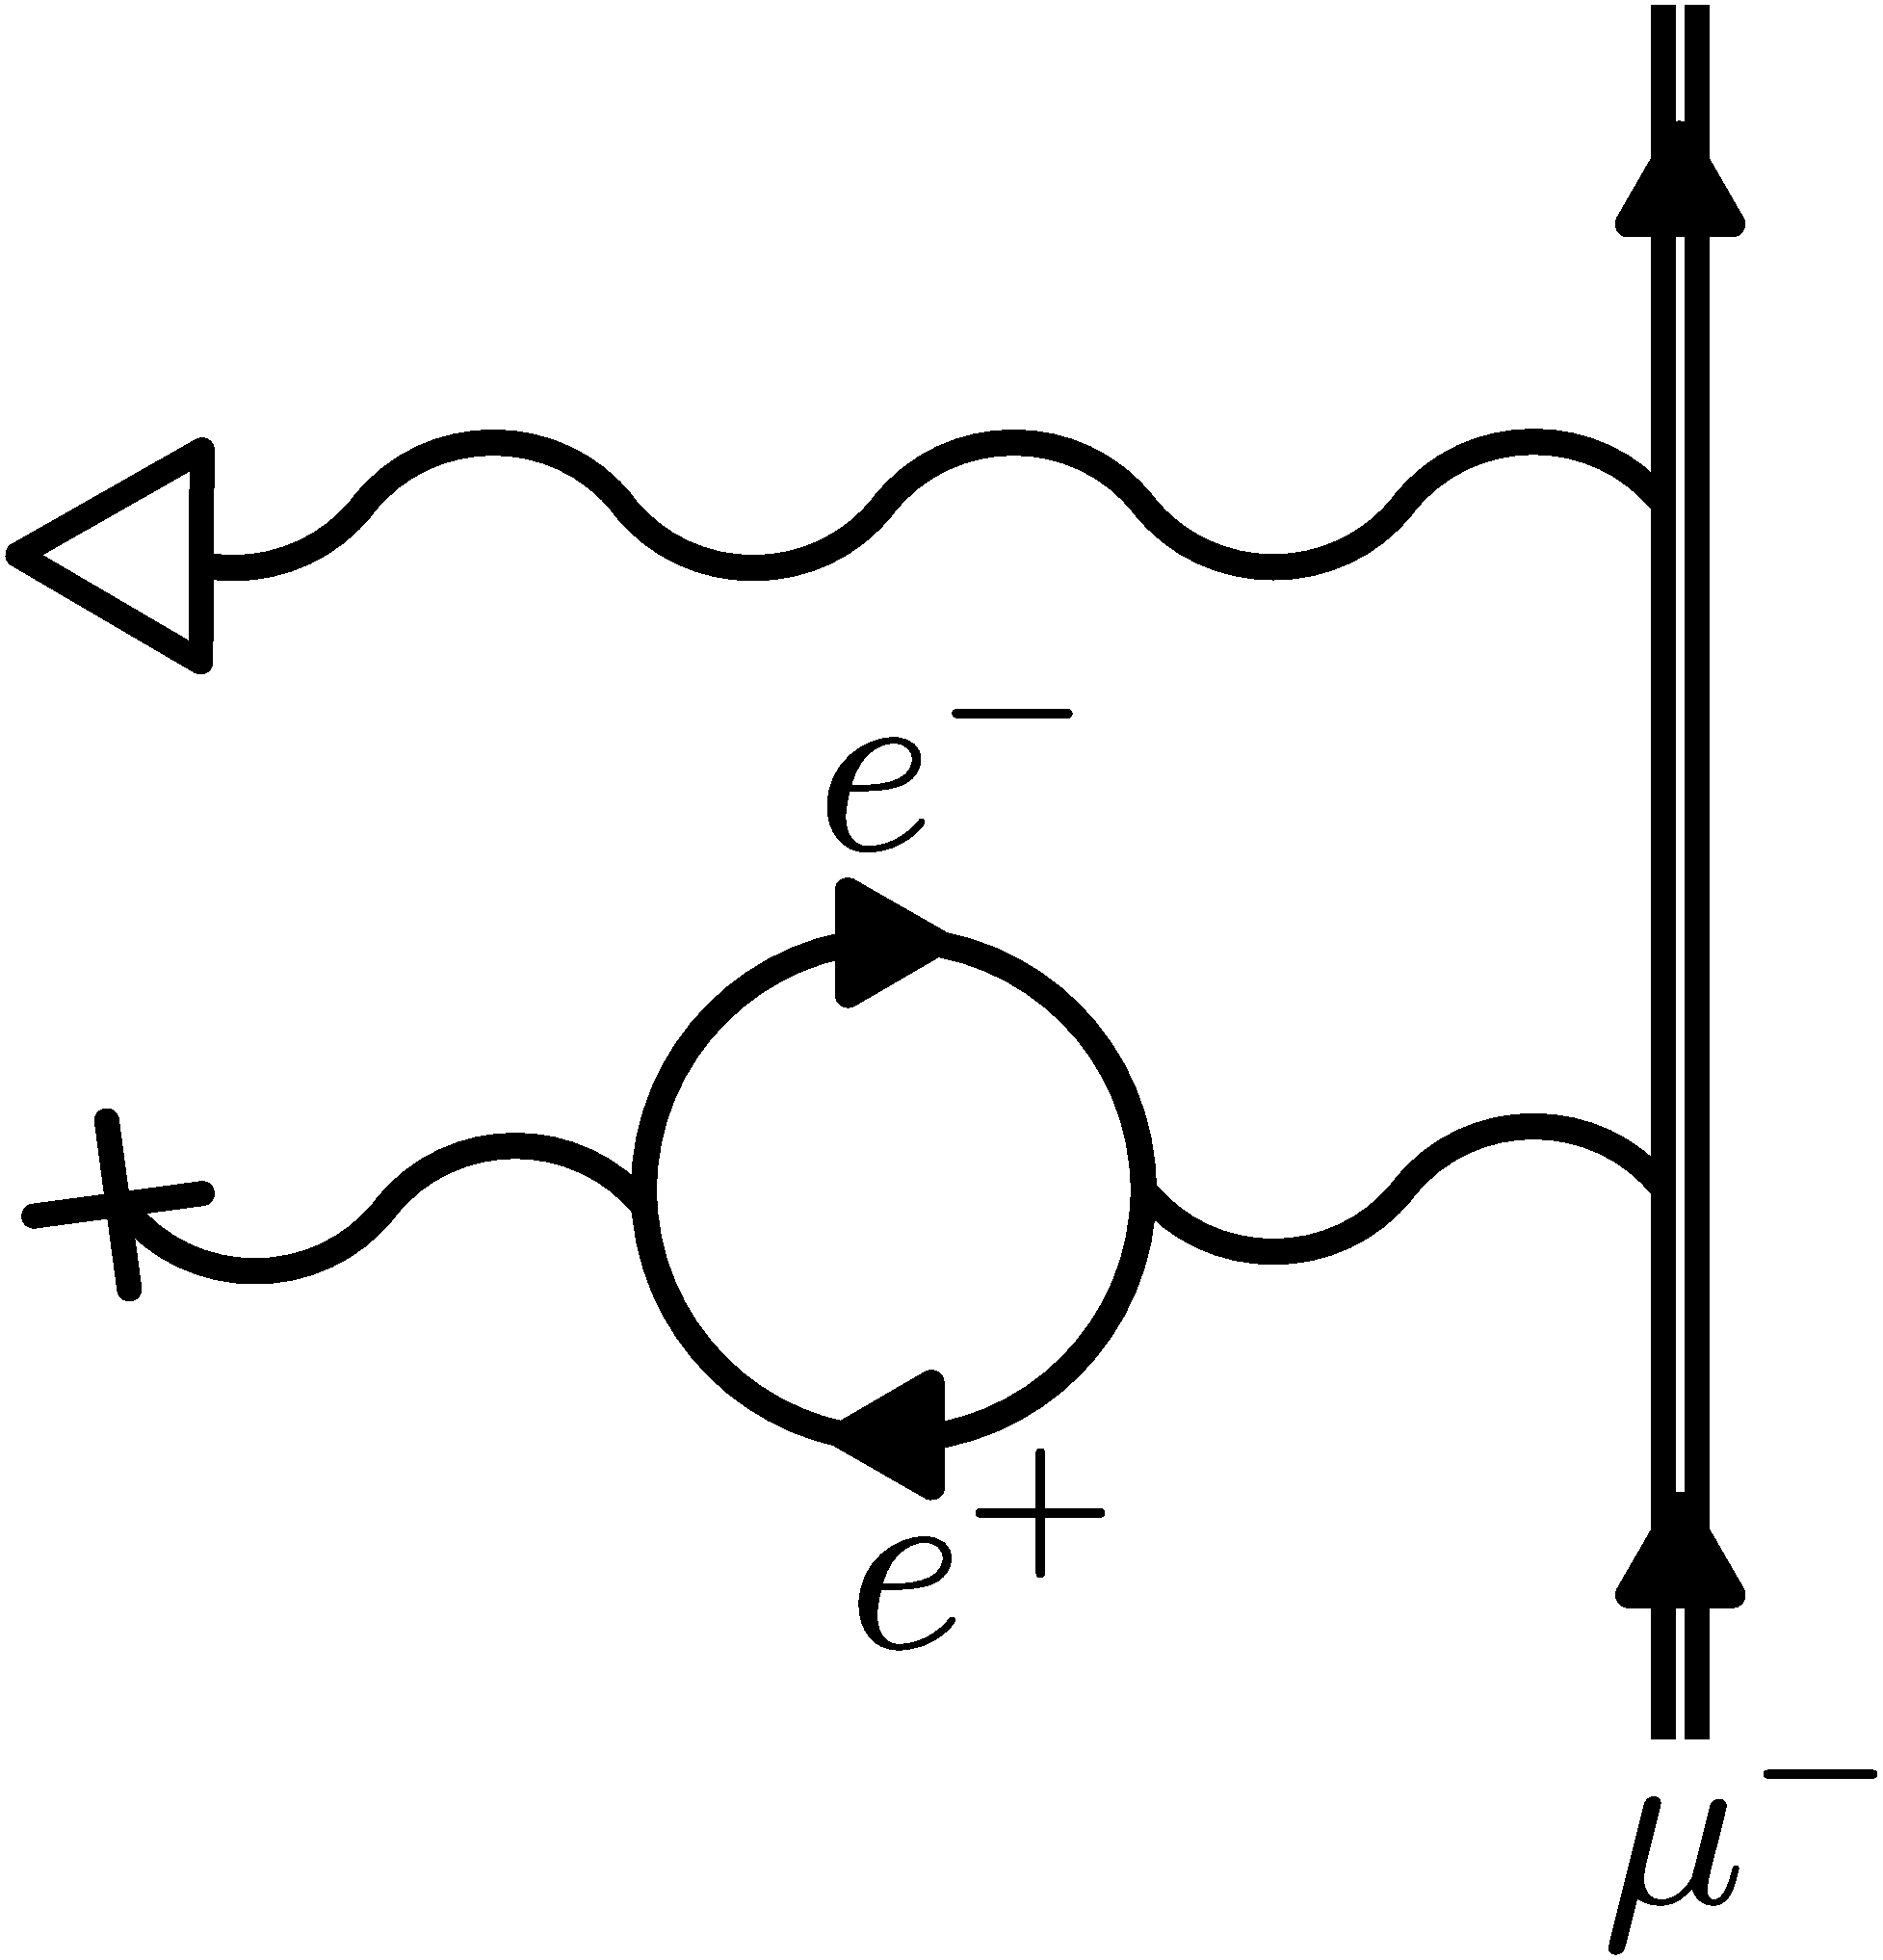
\includegraphics[width=0.22\textwidth]{pics/mixed}\hfill
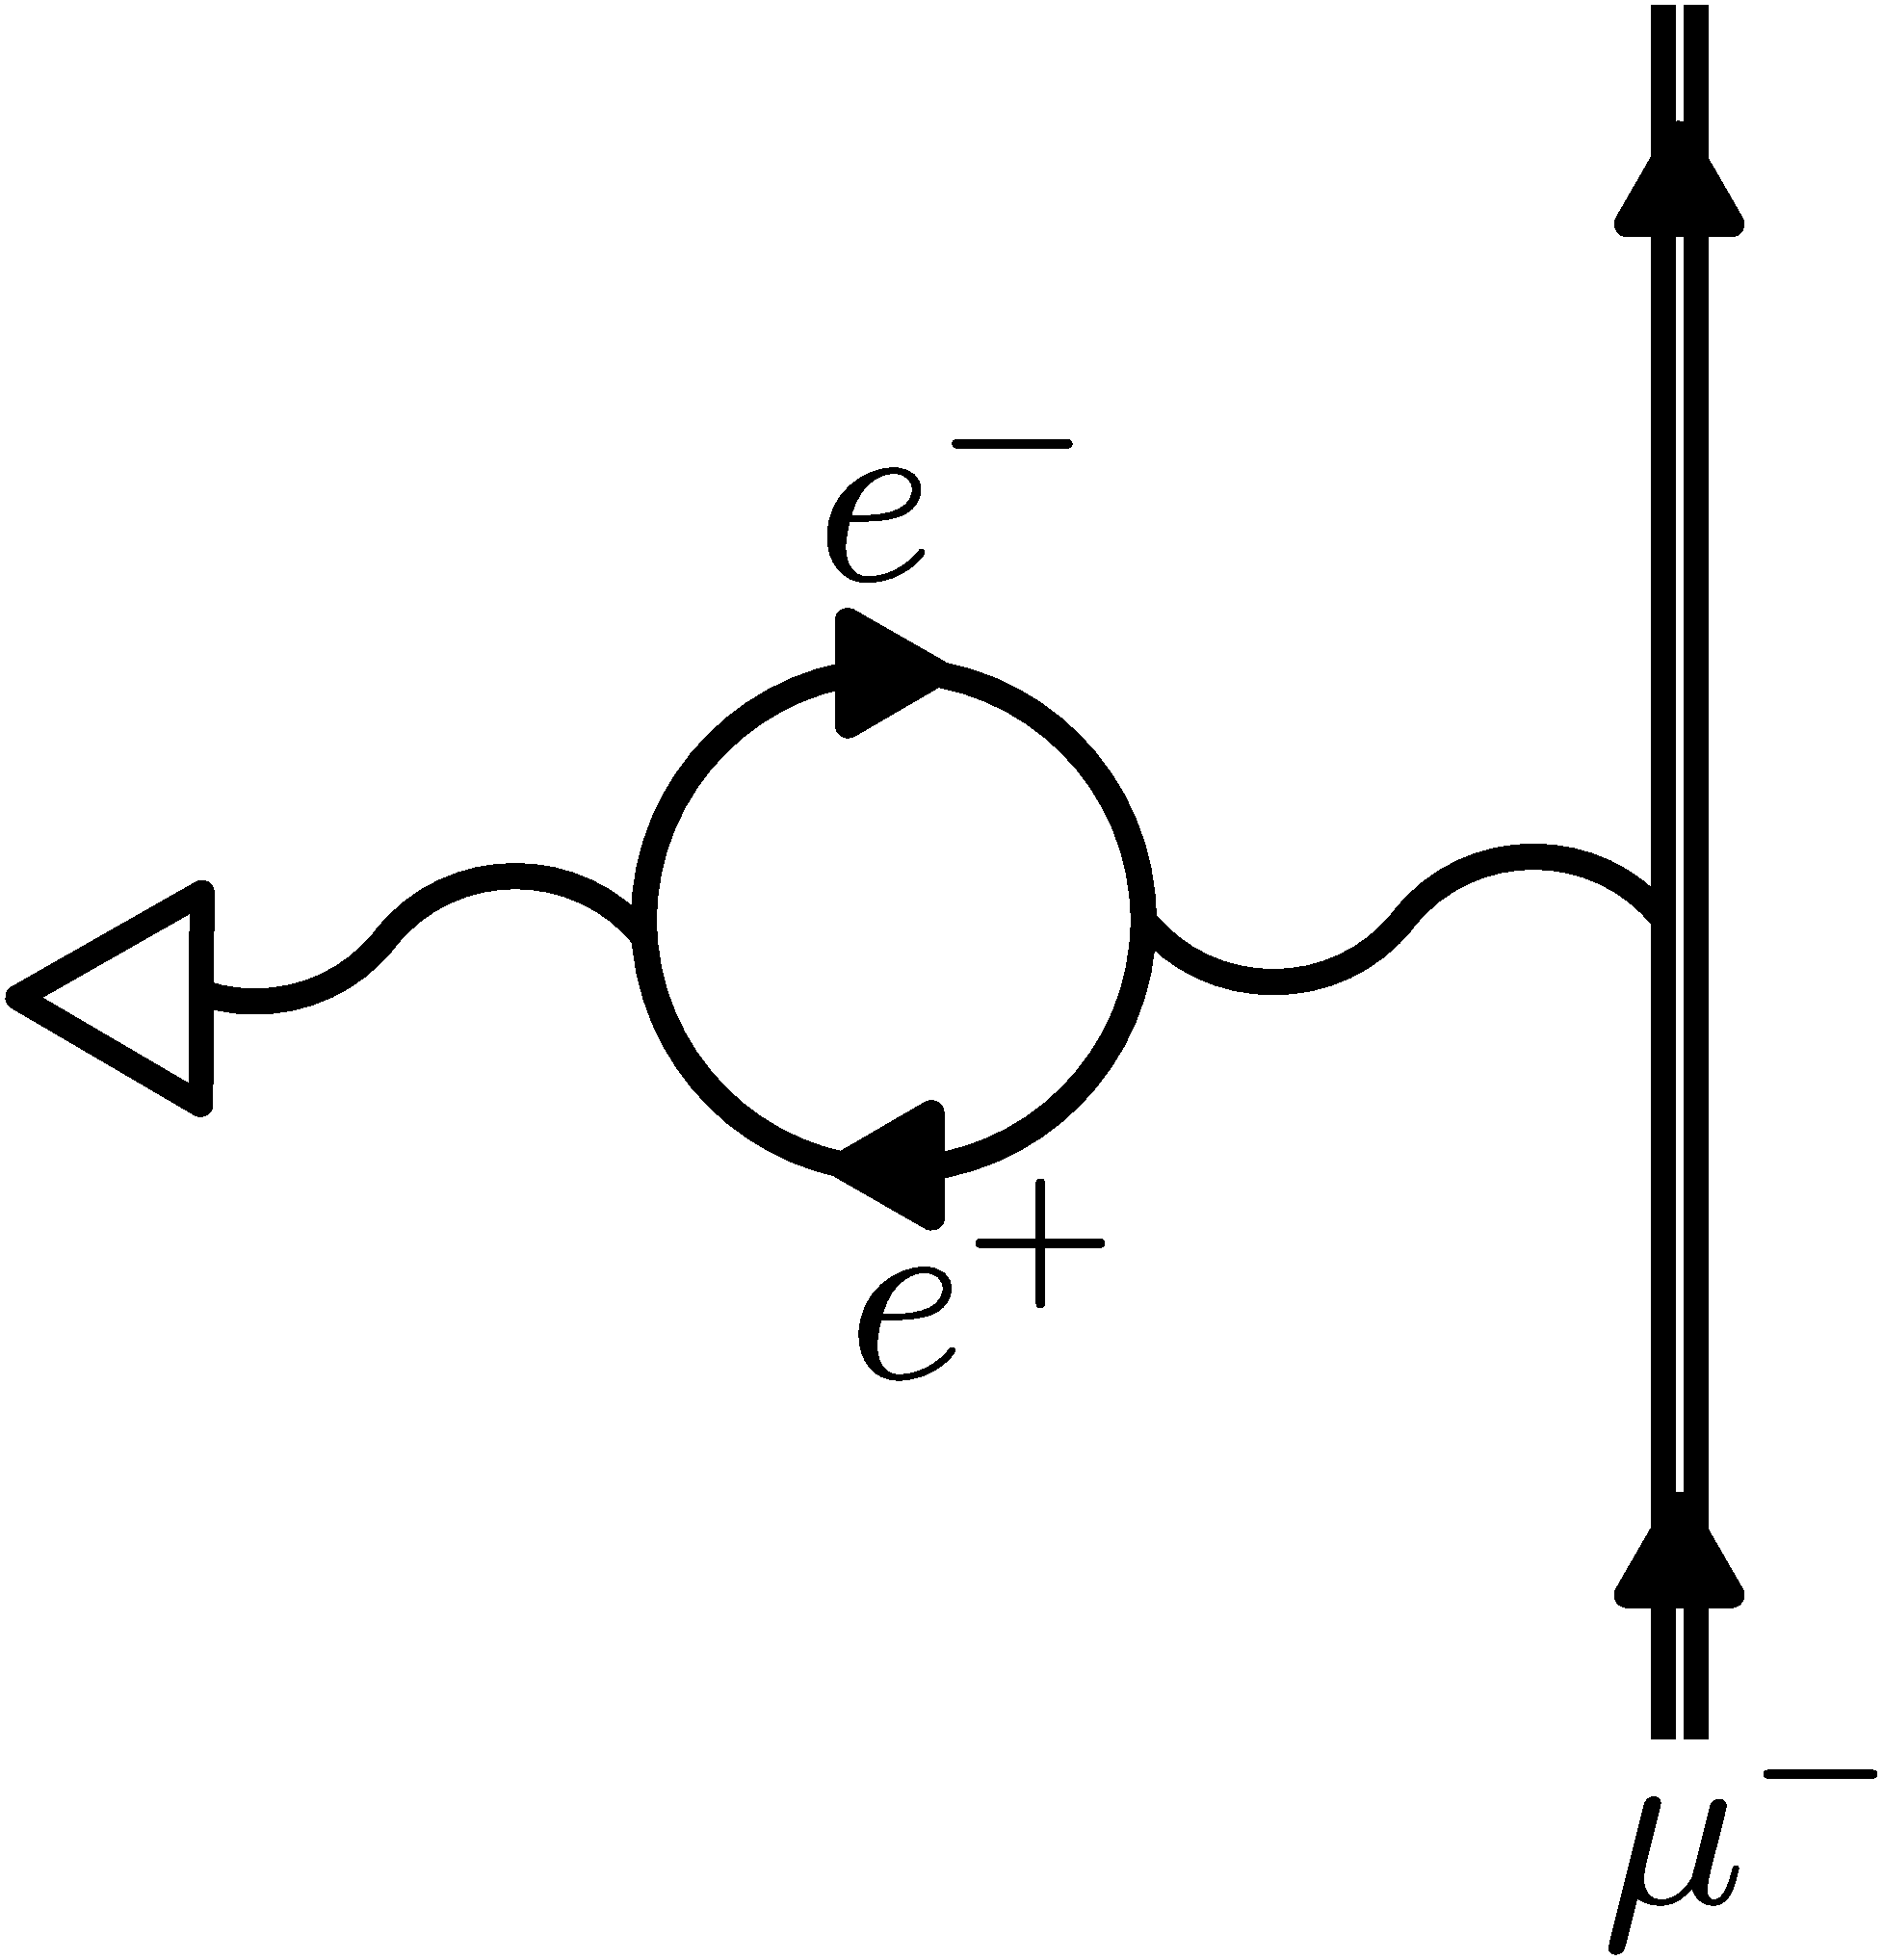
\includegraphics[width=0.22\textwidth]{pics/quehl}\\
$\qquad\qquad\qquad$(a)\hfill(b)$\qquad\qquad\qquad$
\caption{
Feynman diagrams for the leading order contributions of the vacuum polarization to the quadrupole interaction in muonic atoms. An external double line stands for the bound-muon wave function. A single internal line for the free electron propagator, and a wave line for the photon propagator. A cross represents the interaction with the monopole potential, and a triangle the interaction with the quadrupole potential. Contribution (a) is calculated by including the spherically symmetric contribution of the Uehling potential in the Dirac equation~\eqref{eq:h0mu}; Contribution (b) by including the quadrupole contribution of the Uehling potential in the matrix elements from Eq.~\eqref{eq:quadel_uehl} and \eqref{eq:second}.
}
\label{fig:quehl}
\end{figure}
%
%

The monopole terms $V^{(0)}_{\text{el}}(r_\mu)$ and $V^{(0)}_{\text{uehl}}(r_\mu)$ only depend on the muonic radial coordinate and thus were included in this work in the unperturbed muonic states as
\begin{equation}
\left( H_\mu + V^{(0)}_{\text{el}}+V^{(0)}_{\text{uehl}}\right) \left|n\kappa m\right> = E_{n\kappa}\left|n\kappa m \right>,
\label{eq:h0mu}
\end{equation}
where $\left|n\kappa m \right>$ are the solutions of the spherical Dirac equation in terms of the well-known spherical spinors and radial functions $G_{n\kappa}(r_\mu)$ and $F_{n\kappa}(r_\mu)$ with energy $E_{n \kappa}$~\cite{greiner2000}. $n$, $\kappa$, $m$ are the principal quantum number, the relativistic angular quantum number and the $z$ component of the total angular momentum of the muon, respectively. In this way, the monopole Uehling potential and all iterations thereof are included in the muonic wave functions~\cite{michel2017}.
\section{Electric quadrupole interaction}
\subsection{Dynamic Hyperfine structure}
The hyperfine splitting due to electric quadrupole interactions is considered in the coupled basis, where a state with total angular momentum $F$ and its projection on the $z$  axis $M$ is formed for a given muonic and nuclear state as
\begin{equation}
\left| FM\,n\kappa\,IK \right> = \sum_{m,M^\prime} C^{FM}_{jm\,IM^\prime} \left|n\kappa m\right>\otimes\left|IM^\prime K\right>,
\end{equation}
with the Clebsch-Gordan coefficients $C^{jm}_{j_1m_1\,j_2m_2}$. The matrix elements of the electric quadrupole interaction are written as
\begin{equation}
\Delta E^{(2)}_{\text{el}} = \left< FMn_1\kappa_1I_1K\right|{V_{\text{el}}^{(2)}}\left|FMn_2\kappa_2I_2K\right>,
\label{eq:quadel}
\end{equation}
where the diagonal elements correspond to the first order electric hyperfine splitting~\cite{michel2017}. The explicit expressions are given in Eqs.~\eqref{eq:matel} and~\eqref{eq:defmulti} in the Appendix.
\begin{table}[b]
\caption{\label{tab:params}%
Nuclear parameters used in the numerical calculations. $I_0$ is the nuclear ground state angular momentum. RMS and $Q_\text{spec}$ are the nuclear RMS radius and spectroscopic quadrupole moment of the nuclear ground state from~\cite{Angeli2013,Stone2005}, respectively. $c$, $a$, $\beta$ are the parameters of the deformed Fermi distribution derived from RMS and $Q_\text{spec}$, see Sec. \ref{sec:num} for details. $E_{I}$ are the excitation energies of the nuclear rotational states with angular momentum $I$ in Eq.~\eqref{eq:enucl}, the values are taken from~\cite{ENSDF}.}
%\begin{ruledtabular}
\begin{tabular}{rll}
& $^{185}_{\phantom{1}75}$Re & $^{235}_{\phantom{1}92}$U\\ \hline \\[-10pt]
$I_0$ \hfill$\phantom{.}$ & $5/2$ & $7/2$ \\
RMS \hfill[fm] & $5.3596(172)$ & $5.8337(41)$ \\
$Q_\text{spec}$ \hfill[b] & $2.21(4)\phantom{111}$ & $4.936(6)\phantom{1}$ \\
$c$ \hfill[fm] & $6.3517$ & $6.9562$ \\
$a$ \hfill[fm] & 0.5234 & 0.5234 \\
$\beta$ \hfill$\phantom{.}$ & 0.2322 & 0.2711 \\[7pt]
$E_{I_0 + 1}$ \hfill[keV] & 125.3587(9) &  $\phantom{1}$46.108(8) \\
$E_{I_0 + 2}$ \hfill[keV] & 284.2(3) & 103.903(8) \\
$E_{I_0 + 3}$ \hfill[keV] & 475.7(4) & 171.464(13) \\
$E_{I_0 + 4}$ \hfill[keV] & 697.1(5) & 250.014(21) \\
$E_{I_0 + 5}$ \hfill[keV] & 949.7(5) & 339.976(24) \\
\end{tabular}
%\end{ruledtabular}
\end{table}
For heavy, deformed nuclei, the fine structure as well as the first order quadrupole hyperfine structure of muonic energy levels is similar to the energies of the low-lying nuclear rotational states. Therefore, the total Hamiltonian has to be rediagonalized in finite subspaces of a muonic finestructure multiplet and the first few nuclear rotational states. Since multipole interactions are diagonal in $F$ and $M$, there is no mixing of states with different total angular momentum. Thus, if $d$ is the dimension of the subspace, new states
\begin{equation}
\left| FM k \right> := \sum_{i=1}^{d} a^{(k)}_i \left| FM\,n_i\kappa_i\,I_iK \right>
\label{eq:compstate}
\end{equation}
with $k \in {1,...,d}$ may be defined, in which the coefficients $a_i^{(k)}$ have to be chosen such that the matrix representation of the total Hamiltonian \eqref{eq:htot} in the subspace is diagonal. The corresponding eigenenergies are written as $E^{(F,k)}_{\text{quad}}$. This leads to a rich and complex level structure and to hyperfine structure also for nuclei with zero ground-state angular momentum and is know as the dynamic hyperfine structure~\cite{wu1969,Devons1995}.

\subsection{Higher order contributions}
In this work, the VP in Uehling approximation is included in the dynamic hyperfine structure, considering the finite nuclear size. For this, the matrix elements of the quadrupole Uehling interaction
\begin{equation}
\Delta E^{(2)}_{\text{uehl}} = \left< FMn_1\kappa_1I_1K\right|{V_{\text{uehl}}^{(2)}}\left|FMn_2\kappa_2I_2K\right>,
\label{eq:quadel_uehl}
\end{equation}
are added to the matrix elements from Eq.~\eqref{eq:quadel}. The explicit formulas for Eq.~\eqref{eq:quadel_uehl} are given in Eqs.~\eqref{eq:matel} and~\eqref{eq:defmultiuehl} in the Appendix.
By including the monopole Uehling potential in the unperturbed muon states in Eq.~\eqref{eq:h0mu} and the quadrupole Uehling potential in the matrix elements~\eqref{eq:quadel_uehl}, all contributions of the Uehling potential to the electric quadrupole interactions are included, as shown schematically in Fig.~\ref{fig:quehl}~(a) and (b), respectively.

After a subspace has been chosen and rediagonalization has been performed, the quadrupole interaction with states outside of the subspace leads to residual second order corrections to the energy levels~\cite{chen1970}. 
For the total second order correction a summation over the complete (discrete and continous) spectrum for both nuclear and muonic states has to be performed. For the complete nuclear spectrum, sophisticated models or numerous experimental data are required. Therefore, in this work, we calculate the second order corrections, where the nucleus stays in the rotational ground state, but the complete muonic spectrum is considered.
The second order energy shift is
\begin{equation}
\Delta E_{\text{2.ord.}}^{(F,k)}= \sum_i\frac{\left|\left< FMk\right|{V_{\text{el}}^{(2)}}{+}{V_{\text{uehl}}^{(2)}}\left|FMn_i\kappa_iI_iK \right>\right|^2}{E_{F,k}-E_i},
\label{eq:second}
\end{equation}
where the sum is to be taken over all states not considered in the rediagonalization, including continuum states of the muon, and the unperturbed energy of the state $i$ is $E_i=E_{n_i\kappa_i}+E_{I_i}$.
%
%
\section{Numerical Evaluation}
\label{sec:num}
Calculations have been performed for muonic Rhenium and Uranium, assuming a deformed Fermi nuclear charge distribution which reads as
\begin{equation}
\rho_{ca\beta}(\vec{r}\,)=\cfrac{N}{1+\exp (\frac{r-c(1+\beta \text{Y}_{20}(\vartheta))}{a})},
\label{eq:deffermi_2}
\end{equation}
where $c$ is the half-density radius, $a$ the skin thickness, $\beta$ the deformation parameter, and $N$ a normalization constant determined by the condition
\begin{equation}
\int \text{d}^3r\, \rho_{ca\beta}(\vec{r}\,)=1.
\end{equation}
Using the deformed Fermi distribution has proved to be very successful in the description of the level structure of heavy muonic atoms, e.g.~\cite{hitlin1970,tanaka1984,tanaka1984_2}.
Values for the parameters can be estimated by using a value ${a}{=}{2.3\,\text{fm}/(4\ln 3)}$, which has proved to be a sufficiently accurate value for most nuclei~\cite{Beier2000}. Then, $c$ and $\beta$ are chosen such that the quadrupole moment and RMS value of the distribution are in agreement with the literature values from~\cite{Angeli2013,Stone2005}. For the nuclear states involved in the dynamic hyperfine structure, also the excitation energies are needed from literature~\cite{ENSDF}. The used parameters are summarized in Table~\ref{tab:params}.
With these parameters, the electric and Uehling potentials, both monopole and quadrupole parts, can be calculated numerically. The muon wave functions are obtained by solving the Dirac equation~\eqref{eq:h0mu} with the dual-kinetic-balance method~\cite{Shabaev2004}. Thereby, a complete set of muonic bound and continuum states is obtained. An overview for the binding energies of muon states important for the dynamic hyperfine splitting are shown in Table~\ref{tab:monopole}.

\begin{table}[b]
\caption{\label{tab:monopole}%
Binding energies of the low-lying, unperturbed muonic states due to the spherically symmetric parts of the electric and Uehling potential obtained by solving Eq.~\eqref{eq:h0mu} for muonic Rhenium and Uranium. The first column shows the binding energies for a point-like Coulomb potential, the second and third column include the finite size corrections without and with Uehling potential, respectively. See Sec. \ref{sec:num} for details. All energies are in keV.
}
%\begin{ruledtabular}
\begin{tabular}{ccrrr}
& state & \text{point like}& \text{finite size (fs)} &\text{fs+Uehling}\\ \hline \\[-7pt]
$^{185}$Re &1s\nicefrac{1}{2} & 17229.12 & 9333.46 & 9394.02 \\
&2s\nicefrac{1}{2} & 4398.85 & 3083.91 & 3100.44 \\
&2p\nicefrac{1}{2} & 4398.85 & 4032.61 & 4059.50 \\
&2p\nicefrac{3}{2} & 4033.07 & 3885.75 & 3910.50 \\
&3s\nicefrac{1}{2} & 1912.97 & 1498.01 & 1504.28 \\
&3p\nicefrac{1}{2} & 1912.97 & 1789.84 & 1798.66 \\
&3p\nicefrac{3}{2} & 1804.01 & 1751.38 & 1759.75 \\
&3d\nicefrac{3}{2} & 1804.01 & 1802.05 & 1810.30 \\
&3d\nicefrac{5}{2} & 1773.14 & 1772.36 & 1780.16 \\[7pt]
$^{235}$U&1s\nicefrac{1}{2} & 27351.29 & 12100.56 & 12175.51 \\
&2s\nicefrac{1}{2} & 7074.68 & 4308.67 & 4332.13 \\
&2p\nicefrac{1}{2} & 7074.68 & 5901.35 & 5941.39 \\
&2p\nicefrac{3}{2} & 6130.65 & 5674.78 & 5711.89 \\
&3s\nicefrac{1}{2} & 3033.18 & 2148.86 & 2158.31 \\
&3p\nicefrac{1}{2} & 3033.18 & 2645.58 & 2659.26 \\
&3p\nicefrac{3}{2} & 2751.54 & 2588.19 & 2601.27 \\
&3d\nicefrac{3}{2} & 2751.54 & 2739.69 & 2754.06 \\
&3d\nicefrac{5}{2} & 2679.66 & 2674.77 & 2688.10

\end{tabular}
%\end{ruledtabular}
\end{table}
%
%begin hfs table
\begin{table*}
\caption{\label{tab:hfs_2}
Overview of energy corrections due to residual second order electric quadrupole splitting~$\Delta E_{\text{2.ord.}}$ and quadrupole-Uehling interaction~$\Delta E_{\text{quad-uehl}}$ for $^{185}$Re and $^{235}$U. $F$ is the total angular momentum of muon and nucleus, $I_N$ is the nuclear angular momentum and $\mu$-state is the muonic state in spectroscopic notation. For the muonic $2p$ and $3d$ states, these are mixed by the dynamic hyperfine structure, thus $I_N$ (main) and $\mu$-state (main) show the states with the largest contribution. $E_{\text{quad}}$ is the binding energy without quadrupole Uehling and residual second order quadrupole interaction, see Sec. \ref{sec:num} for details. The states are ordered descending in the total energy~$E_{\text{tot}}$. All energies are in keV.}
%\begin{ruledtabular}
\begin{tabular}{lrccccc|c}
 &F&\multicolumn{1}{c}{$I_{N}\,\text{(main)}$}&$\mu\text{-state (main)}$&\multicolumn{1}{c}{$E_{\text{quad}}$}&\multicolumn{1}{c}{$\Delta E_{\text{2.ord.}}$}&\multicolumn{1}{c}{$\Delta E_{\text{quad-uehl}}$}&\multicolumn{1}{c}{$E_{\text{tot}}$}\\\hline\\[-7pt]
$^{185}\text{Re}$&  2 &   \nicefrac{5}{2} & 1s\nicefrac{1}{2} & 9394.02 &  3.21 &   0.00 & 9397.23 \\
&  6 &  \nicefrac{13}{2} & 1s\nicefrac{1}{2} & 8696.92 &  2.06 &   0.00 & 8698.98 \\
&  8 &  \nicefrac{15}{2} & 1s\nicefrac{1}{2} & 8444.32 &  1.76 &   0.00 & 8446.08 \\
&  2 &   \nicefrac{5}{2} & 2p\nicefrac{1}{2} & 4083.31 &  2.18 &  0.28 & 4085.77 \\
&  3 &   \nicefrac{5}{2} & 2p\nicefrac{1}{2} & 4077.79 &  2.07 &  0.23 & 4080.09 \\
&  3 &   \nicefrac{9}{2} & 2p\nicefrac{3}{2} & 3992.27 &  2.41 &  0.41 & 3995.09 \\
&  4 &   \nicefrac{7}{2} & 2p\nicefrac{1}{2} & 3957.33 &  2.10 &  0.26 & 3959.69 \\
&  3 &   \nicefrac{5}{2} & 2p\nicefrac{3}{2} & 3886.35 &  1.12 & -0.22 & 3887.25 \\
&  5 &   \nicefrac{7}{2} & 2p\nicefrac{3}{2} & 3814.27 &  2.08 &  0.28 & 3816.63 \\
&  4 &   \nicefrac{9}{2} & 2p\nicefrac{1}{2} & 3734.93 &  1.03 & -0.27 & 3735.69 \\
&  6 &   \nicefrac{9}{2} & 2p\nicefrac{3}{2} & 3650.57 &  1.95 &  0.25 & 3652.77 \\
&  5 &   \nicefrac{9}{2} & 2p\nicefrac{3}{2} & 3556.36 &  1.13 & -0.24 & 3557.25 \\
&  7 &  \nicefrac{11}{2} & 2p\nicefrac{3}{2} & 3458.14 &  1.85 &  0.23 & 3460.22 \\
&  6 &  \nicefrac{11}{2} & 2p\nicefrac{3}{2} & 3344.35 &  0.93 & -0.19 & 3345.09 \\
&  8 &  \nicefrac{13}{2} & 2p\nicefrac{3}{2} & 3111.03 &  0.68 &  0.02 & 3111.73 \\
&  7 &  \nicefrac{15}{2} & 2p\nicefrac{3}{2} & 2941.66 &  0.82 & -0.15 & 2942.33 \\
&  8 &  \nicefrac{15}{2} & 2p\nicefrac{3}{2} & 2938.52 &  0.67 & -0.16 & 2939.03 \\
&  3 &   \nicefrac{5}{2} & 3d\nicefrac{3}{2} & 1815.47 &  0.07 &  0.03 & 1815.57 \\
&  1 &   \nicefrac{5}{2} & 3d\nicefrac{3}{2} & 1804.28 &  0.11 & -0.03 & 1804.36 \\
&  3 &   \nicefrac{7}{2} & 3d\nicefrac{5}{2} & 1783.72 &  0.05 &  0.02 & 1783.79 \\
&  0 &   \nicefrac{5}{2} & 3d\nicefrac{5}{2} & 1772.11 &  0.11 & -0.04 & 1772.18 \\[7pt]
$^{235}\text{U}$&  3 &   \nicefrac{7}{2} & 1s\nicefrac{1}{2} & 12175.51 &  6.83 &   0.00 & 12182.34 \\
&  7 &  \nicefrac{15}{2} & 1s\nicefrac{1}{2} & 11925.50&  4.66 &  0.00  & 11930.16 \\
&  9 &  \nicefrac{17}{2} & 1s\nicefrac{1}{2} & 11835.54&  3.54 &  0.00  & 11839.08 \\
&  3 &   \nicefrac{7}{2} & 2p\nicefrac{1}{2} & 6019.06 &  5.99 &  0.85 & 6025.90 \\
&  4 &   \nicefrac{7}{2} & 2p\nicefrac{1}{2} & 6015.01 &  5.96 &  0.83 & 6021.80 \\
&  4 &   \nicefrac{9}{2} & 2p\nicefrac{1}{2} & 5979.31 &  6.02 &  0.86 & 5986.19 \\
&  5 &   \nicefrac{9}{2} & 2p\nicefrac{3}{2} & 5928.94 &  6.06 &  0.88 & 5935.88 \\
&  6 &  \nicefrac{11}{2} & 2p\nicefrac{3}{2} & 5868.85 &  6.00 &  0.89 & 5875.74 \\
&  7 &  \nicefrac{15}{2} & 2p\nicefrac{1}{2} & 5798.66 &  5.30 &  0.91 & 5804.87 \\
&  8 &  \nicefrac{15}{2} & 2p\nicefrac{1}{2} & 5745.59 &  4.71 &  0.87 & 5751.17 \\
&  5 &   \nicefrac{7}{2} & 2p\nicefrac{3}{2} & 5673.10 &  3.12 & -0.42 & 5675.80 \\
&  6 &   \nicefrac{9}{2} & 2p\nicefrac{3}{2} & 5621.02 &  3.02 & -0.46 & 5623.58 \\
&  2 &   \nicefrac{7}{2} & 2p\nicefrac{3}{2} & 5620.12 &  2.78 & -0.56 & 5622.34 \\
&  9 &  \nicefrac{17}{2} & 2p\nicefrac{1}{2} & 5613.24 &  2.05 &  0.13 & 5615.42 \\
&  3 &   \nicefrac{9}{2} & 2p\nicefrac{3}{2} & 5586.28 &  2.81 & -0.54 & 5588.55 \\
&  7 &  \nicefrac{13}{2} & 2p\nicefrac{1}{2} & 5556.38 &  2.60 & -0.50 & 5558.48 \\
&  9 &  \nicefrac{15}{2} & 2p\nicefrac{3}{2} & 5493.59 &  2.44 &  0.24 & 5496.27 \\
&  8 &  \nicefrac{15}{2} & 2p\nicefrac{1}{2} & 5479.30 &  2.14 & -0.53 & 5480.91 \\
& 10 &  \nicefrac{17}{2} & 2p\nicefrac{3}{2} & 5393.16 &  1.77 &  0.13 & 5395.06 \\
&  9 &  \nicefrac{17}{2} & 2p\nicefrac{3}{2} & 5315.81 &  1.73 & -0.44 & 5317.10 \\
&  3 &   \nicefrac{7}{2} & 3d\nicefrac{3}{2} & 2767.16 &  0.44 &  0.09 & 2767.69 \\
&  1 &   \nicefrac{7}{2} & 3d\nicefrac{5}{2} & 2663.35 &  0.61 & -0.13 & 2663.83 \\
\end{tabular}
%\end{ruledtabular}
\end{table*}
% end hfs table
The quadrupole matrix elements from Eq.~\eqref{eq:quadel} can be calculated both for the rediagonalization in the dynamic hyperfine structure and for the evaluation of the residual second-order terms \eqref{eq:second}, using Eq.~\eqref{eq:matel}. As the next step, the total Hamiltonian~\eqref{eq:htot} is diagonalized in finite subspaces or modelspaces consisting of the muonic ($2p\nicefrac{1}{2}$, $2p\nicefrac{3}{2}$) or ($3d\nicefrac{3}{2}$, $3d\nicefrac{5}{2}$) doublet states and nuclear ground state rotational band. For Rhenium, the first six states with $I_N \in \{5/2,...,15/2\}$ are considered, and for Uranium with $I_N \in \{7/2,...,17/2\}$. The excitation energies of the nuclear states are summarized, along with other nuclear parameters, in Table~\ref{tab:params}. Thereby, the composite states and corresponding energies $E_{\text{quad}}$ from Eq.~\eqref{eq:compstate} are obtained and finally, for each of these states the residual second order quadrupole correction \eqref{eq:second} is calculated. Here, the intermediate sum goes over all nuclear and muonic states not included in the modelspace.
Note that for the muonic ground state, a rediagonalization is not necessary, since the diagonal matrix elements of the quadrupole interactions vanish for muonic states with $j=1/2$.
The quadrupole-Uehling contribution to the binding energies can be obtained by performing the calculations for the dynamic hyperfine structure twice; once with the matrix elements~\eqref{eq:quadel} and~\eqref{eq:quadel_uehl} containing both the electric and Uehling interaction ${V_{\text{el}}^{(2)}}{+}{V_{\text{uehl}}^{(2)}}$ and a second time only with the electric part ${V_{\text{el}}^{(2)}}$ from Eq.\eqref{eq:quadel}. The difference between those two approaches gives the quadrupole-Uehling corrections. Results for the residual second order quadrupole correction from Eq.~\eqref{eq:second} and for the quadrupole-Uehling corrections can be found in Table~\ref{tab:hfs_2} for a number of states.
\section{Discussion and Summary}
The quadrupole interaction in the framework of the dynamic hyperfine structure in heavy muonic atoms was analyzed by an fully relativistic treatment of the quadrupole-Uehling potential and of the residual second order terms.
The quadrupole-Uehling interaction was obtained by a multipole expansion of the Uehling potential for an arbitrary nuclear charge distribution without the assumption on the distance between muon and nuclear charge being large.
Since it has the same angular structure as the conventional quadrupole interaction, the quadrupole-Uehling expectation value vanishes between two muonic states with $j=1/2$, thus it does not affect the muonic ground state.
The calculations for Uranium show that it can lead to energy corrections almost on the keV level for very heavy nuclei with muonic $2p$ states and thus can be potentially relevant for comparison between theoretical predictions and experiments. Being a short-ranged potential, it falls of quickly for states further away from the nucleus. For states with $n\geq3$, we find values below $0.15\,$keV, even for high Z.
The generalization to Uehling corrections for higher order multipole is straight forward. In the case of muonic atoms, since the influence of higher order multipoles is already small, we expect this correction will not contribute significantly.

The residual second order quadrupole corrections in the dynamic hyperfine structure were calculated numerically using a basis of relativistic wave functions including nuclear finite size correction and Uehling correction due to the monopole part of the nuclear potential.
In contrast to the first order terms, the muonic ground state energy is affected by the second order corrections. Here, the energy correction amounts up to several keV. Also for muonic $2p$ states, it is of similar size. For the $3d$ levels, we find the energy corrections below half a keV, both for Rhenium and Uranium.
If a more complete nuclear model instead the rotational model is used, the additional nuclear states appear as intermediate state in the second order corrections, leading to the nuclear polarization corrections. Therefore, the approach presented in this work provides a basis for an accurate treatment of the muonic spectrum for the nuclear polarization effect in deformed muonic atoms.

\section{Multipole expansion of electric \\and Uehling potential}
\label{sec:multipole}
With the multipole expansion of the Coulomb potential~\cite{jackson1999}
\begin{equation}
\frac{1}{|\vec{r}_\mu^{\,\prime}-\vec{r}_N^{\,\prime}|}=\sum_{l=0}^\infty \frac{r_<^l}{r_>^{l+1}}\sum_{m=-l}^l  \text{C}^*_{lm}(\vartheta_N^{\prime},\varphi_N^{\prime})\text{C}_{lm}(\vartheta_\mu^\prime,\varphi_\mu^\prime),
\end{equation}
where $r_<:=\min (r_\mu,r_N)$, $r_>:=\max (r_\mu,r_N)$, the electric potential~\eqref{eq:pot} can be written as
\begin{align}
V_{\text{el}}(\vec{r}_\mu^{\,\prime})=&\sum_{l,m}-Z\alpha \left[ \int \text{d}^3r^{\prime}_N \frac{r_<^l}{r_>^{l+1}}\text{C}^*_{lm}(\vartheta_N^{\prime},\varphi_N^{\prime})\rho(\vec{r}_N^{\,\prime})\right]\notag\\
&\,\times\text{C}_{lm}(\vartheta_\mu^{\prime},\varphi_\mu^\prime),
\end{align}
where ${\text{C}_{lm}(\vartheta,\varphi)}{=}{\sqrt{4\pi/(2l+1)}\text{Y}_{lm}(\vartheta,\varphi)}$ are the normalized spherical harmonics and primed coordinates belong to the nuclear body-fixed system.
For axially symmetric charge distributions, only the ${m}{=}{0}$-terms are non-zero after integrating over the charge distribution. The dependency on the muonic angular variables can be transformed to the laboratory system by
\begin{equation}
\text{P}_{l}(\cos\vartheta_\mu^\prime)=
 \sum_{m=-l}^l C^*_{lm}(\theta,\phi)C_{lm}(\vartheta_\mu,\varphi_\mu).
\end{equation}
Thereby, the potential as a function of the Euler angles and the muon's position in the laboratory frame reads
\begin{align}
V_{\text{el}}(\vec{r}_\mu,\phi,\theta)=&\sum_{l=0}^\infty-Z\alpha \left[ \int \text{d}^3r^{\prime}_N \frac{r_<^l}{r_>^{l+1}}\text{P}_{l}(\cos \vartheta_N^{\prime})\rho(\vec{r}_N^{\,\prime})\right]\notag\\
&\quad\,\times \sum_{m=-l}^l \text{C}^*_{lm}(\theta,\phi)\text{C}_{lm}(\vartheta_\mu,\varphi_\mu).\notag\\
=:&\sum_{l=0}^\infty Q_{\text{el}}^{(l)}(r_\mu)\sum_{m=-l}^lC^*_{lm}(\theta,\phi)C_{lm}(\vartheta_\mu,\varphi_\mu)&\notag\\
=:& \sum_{l=0}^\infty V^{(l)}_{\text{el}}(\vec{r}_\mu,\phi,\theta),
\label{eq:defmulti}
\end{align}
where $Q_{\text{el}}^{(l)}(r_\mu)$ describe the radial distribution of the mulitpole moments.

The Uehling potential can be expanded in multipoles in a similar way, now with a different dependence on $|\vec{r}_\mu^{\,\prime}-\vec{r}_N^{\,\prime}|$, as
\begin{align}
\frac{K_1(2m_e{|\vec{r}_\mu^{\,\prime} - \vec{r}^{\,\prime}\,|})}{|\vec{r}_\mu^{\,\prime} - \vec{r}^{\,\prime}\,|}
&=\sum_{l=0}^\infty c_l(r_\mu,r_N)\\
&\times\sum_{m=-l}^l \text{C}^*_{lm}(\vartheta_N^{\prime},\varphi_N^{\prime})\text{C}_{lm}(\vartheta_\mu^\prime,\varphi_\mu^\prime).\notag
\end{align}
The expansion coefficients $c_l$ can be calculated, using the fact that rotations do not change the absolute value of vectors, as
\begin{equation}
|\vec{r}_\mu^{\,\prime} - \vec{r}_N^{\,\prime}|
=|\vec{r}_\mu - \vec{r}_N|
=\sqrt{r_\mu^2 + r_N^2 - 2 r_\mu r_N y},
\end{equation}
with ${y}{=}{\cos(\sphericalangle \vec{r}_\mu\vec{r}_N)}$ being the cosine of the angle between the vectors $\vec{r}_\mu$ and $\vec{r}_N$, and read as
\begin{equation}
c_l(r_\mu,r_N)=\frac{2l+1}{2} \int_{-1}^1 \text{d}y \frac{K_1(2m_e{|\vec{r}_\mu - \vec{r}_N|})}{|\vec{r}_\mu - \vec{r}_N|} P_l(y),
\label{eq:defcl}
\end{equation}
and are evaluated by numerical integration.
Thereby, the Uehling potential can be written, analogously to Eq.~\eqref{eq:defmulti}, as
\begin{align}
V_{\text{uehl}}(\vec{r}_\mu,\phi,\theta)=&\sum_{l=0}^\infty-Z\alpha\frac{2\alpha}{3\pi} \notag\\
&\quad\times\left[ \int \text{d}^3r^{\prime}_N c_l(r_\mu,r_N)\text{P}_{l}(\cos \vartheta_N^{\prime})\rho(\vec{r}_N^{\,\prime})\right]\notag\\
&\quad\,\times \sum_{m=-l}^l \text{C}^*_{lm}(\theta,\phi)\text{C}_{lm}(\vartheta_\mu,\varphi_\mu).\notag\\
=:&\sum_{l=0}^\infty Q^{(l)}_{\text{uehl}}(r_\mu)\times\sum_{m=-l}^lC^*_{lm}(\theta,\phi)C_{lm}(\vartheta_\mu,\varphi_\mu)&\notag\\
=:& \sum_{l=0}^\infty V^{(l)}_{\text{uehl}}(\vec{r}_\mu,\phi,\theta).
\label{eq:defmultiuehl}
\end{align}
For $l=0$, the expression for Uehling potential of a spherical charge distribution~\cite{Fullerton1976} which only depends on $r_\mu$ is recovered as
\begin{align}
\label{eq:sph_uehl}
V^{(0)}_{\text{uehl}}(r_\mu)=& -\frac{2\alpha (Z\alpha)}{3 m_e r}\int_0^\infty \text{d}r^{\prime}\,\rho_0(r^\prime)\\
&\times\left[K_0(2m_e|r-r^\prime|)-K_0(2m_e(r+r^\prime))\right]\notag
\end{align}
where the spherically averaged part of the charge distribution is
\begin{equation}
\rho_0(r)=\int_0^{2\pi}\text{d}\varphi\int_0^\pi\text{d}\vartheta \sin(\vartheta)\rho(\vec{r}\,)/(4\pi).
\end{equation}
%
%
\section{Matrix elements\\of quadrupole interactions}
\label{sec:mat}
Both the electric and Uehling multipole interaction are a scalar product of rank-$l$ spherical tensors in the angular variables of the muon and of the nucleus. Thus, their matrix elements in states of defined total angular momentum can be reduced to a product of two reduced matrix elements~\cite{varshalovich1988} as
\begin{align}
&{\left< F_1M_1n_1\kappa_1I_1K\right|V^{(l)}(\vec{r}_\mu,\phi,\theta)\left|FMn_2\kappa_2I_2K\right>} {=}
{\delta_{\scriptscriptstyle F_1F_2}\delta_{\scriptscriptstyle M_1M_2}}\notag\\
&\qquad\times(-1)^{F_1+j_2+I_1}
\left\{
\begin{matrix}
j_1&j_2&l\\
I_1&I_2&F_1
\end{matrix}
\right\}\left< I_1K\big{|}\big{|}\text{C}_l(\theta,\phi)\big{|}\big{|}I_2K\right>\notag\\
&\qquad\times \left< n_1\kappa_1\big{|}\big{|}Q^{(l)}(r_\mu)\text{C}_l(\vartheta_\mu,\varphi_\mu) \big{|}\big{|}n_2\kappa_2\right>.\label{eq:matel}
\end{align}
The matrix elements for the nucleus, reduced in $M$ but not in $K$, read~\cite{brown_carrington}
\begin{align}
\left< I_1K\big{|}\big{|}\text{C}_l(\theta,\phi)\big{|}\big{|}I_2K\right>=&(-1)^{I_2+K}
\sqrt{(2I_1+1)(2I_2+1)}\notag\\
&\times\,\left(
\begin{matrix}
I_1&I_2&l\\
-K&K&0
\end{matrix}
\right),
\end{align}
and the reduced matrix elements in the muonic variables are~\cite{johnson2007}
\begin{align}
&\left< n_1\kappa_1\big{|}\big{|}Q^{(l)}(r_\mu)\text{C}_l(\vartheta_\mu,\varphi_\mu) \big{|}\big{|}n_2\kappa_2\right> =  \\
&\quad (-1)^{j_1+1/2} \sqrt{(2j_1+1)(2j_2+1)}
\left(
\begin{matrix}
j_1&j_2&l\\
-\frac{1}{2}&\frac{1}{2}&0
\end{matrix}
\right)\notag\\
&\quad\times\,
\int \text{d}rr^2 ({g_{n_1\kappa_1}(r)g_{n_2\kappa_2}(r)}{+}{f_{n_1\kappa_1}(r)f_{n_2\kappa_2}(r)}) Q^{(l)}(r_\mu),\notag
\end{align}
where $g_{n\kappa}(r)$ and $f_{n\kappa}(r)$ are the two radial functions of the solutions of the Dirac equation in the spherically symmetric potential~\cite{greiner2000} from Eq.~\eqref{eq:h0mu}.






 
  

  \cleardoublepage
  \phantomsection
  \addcontentsline{toc}{chapter}{Summary \& Outlook} %\protect\large
  \chapter*{Summary \& Outlook}
\markboth{Summary \& Outlook}{}
\label{ch:conclusion}

%\subsubsection*{Summary}
In the present thesis, nuclear structure effects caused by extended and deformed nuclear charge distributions and corrections from quantum electrodynamics in the spectra of heavy ions and muonic atoms are investigated. 
Here, the focus is on two topics, namely, on the analysis of the level structure and spectra of muonic atoms, and on improved calculations of the nuclear shape effect on the bound-electron $g$ factor for spinless nuclei beyond the previously used perturbative evaluation.\\[11pt]%
%
Chapter~\ref{ch:muonic_atoms} deals with high-precision calculations of the spectra of muonic atoms. 
As a first step, the implementation of the most important effects, namely, finite nuclear size, vacuum polarization, recoil, and electron screening on the fine and hyperfine structure is discussed in Sec.~\ref{sec:calculationSpectraMuon}.
This includes calculations of the dynamical hyperfine structure, which means that the hyperfine structure is considered beyond the first order in the quadrupole interaction for the most important states.
A finite-basis-set method based on B-splines has been used, which is a well established and efficient method in atomic physics, but had not been used in the context of muonic atoms before. Thereby, a practical, numerical representation of the complete spectrum of muon wave functions is obtained.

In Sec.~\ref{sec:higherorder}, enhanced theoretical approaches for calculations connected to the electric quadrupole interaction between muon and nucleus are presented. 
Firstly, this includes a numerical evaluation of the leading-order vacuum polarization correction (Uehling potential) to the quadrupole matrix elements for an arbitrary, deformed nuclear charge distribution. In contrast to previous works, this is done without any approximations on the shape of the charge distribution or the distance between nucleus and muon. For this, a multipole expansion of the Uehling potential is performed. In this thesis, the corresponding expansion coefficients are given in a form suitable for numerical evaluation, as well as analytically in terms of special functions.
Secondly, the energy correction due to residual second-order quadrupole interaction is calculated by means of the finite basis set of muon wave functions.
Both contributions are shown to be potentially important for upcoming experiments.

In Sec.~\ref{sec:muon_re}, the theoretical calculations of this thesis are compared to state-of-the-art experiments in muonic atom spectroscopy, performed recently at the Paul Scherrer Institute (Switzerland) by the MuX collaboration. Theoretical spectra have been fitted to experimental ones by adjusting the parameters of the nuclear model. In this way, the nuclear quadrupole moment of $_{\phantom{1}75}^{185}$Re and $_{\phantom{1}75}^{187}$Re were extracted from the observed ${n}{=}{5}\rightarrow {n}{=}{4}$ x-rays. Obtaining values for the nuclear quadrupole moments is of great importance, because they can be tested against predictions from theoretical nuclear models. 
Also, the spectra of low-lying muonic x-rays in $_{\phantom{1}75}^{185}$Re have been explained by the calculations in this thesis.\\[11pt]%
%
Chapter~\ref{ch:nucl_def} covers non-perturbative calculations of nuclear shape effects on the bound-electron $g$ factor. Here, the previously used perturbative method is introduced, which is called the effective-radius method, because the homogeneously charged sphere model of a given radius with approximately the same energy correction as the deformed nuclear charge distribution is used. 
Then, the non-perturbative, numerical method used in this thesis is explained, wherein the nuclear potential, the solution of the Dirac equation and the corresponding $g$ factor are calculated in an all-numeric manner, starting with the deformed nuclear charge distribution. Calculations for a wide range of nuclei across the nuclear chart reveal that the perturbative evaluation overestimated the nuclear shape effect on the 20\% level. The difference between the fully numerical and perturbative, effective-radius method is investigated. It is shown that the formulas for a perturbative calculation of the effective radius and the corresponding energy correction of the homogeneously charged sphere are mainly responsible for the disagreement, but also the incompleteness of the effective radius method itself contributes.

Furthermore, the connection between nuclear finite size and deformation effects is discussed and it is demonstrated how the consideration of deformed nuclei can reduce the model uncertainty in the theoretical prediction of finite-nuclear-size effects on the bound-electron $g$ factor. The previous, conservative estimation of this uncertainty is the difference in the $g$ factors due to a homogeneously charged sphere and a Fermi-type nuclear charge distribution. If parameters of the deformed nuclear charge distribution are available, the finite-nuclear-size and shape $g$-factor corrections can be calculated with their help. In this way, the remaining model uncertainty is reduced due to the more realistic nuclear model, which is demonstrated with calculations for hydrogen-like uranium.\\[11pt]%
%
Finally, in Chapter~\ref{sec:muon_he}, finite nuclear size and several vacuum polarization corrections to the bound-muon $g$ factor in muonic helium are presented. In combination with other calculations, this enabled a theoretical prediction of the $g$ factor on the $10^{-9}$ level. It has been shown that not only the finite nuclear size and first-order Uehling correction are important on this level of accuracy, but also the two-loop Uehling and Källén-Sabry corrections, evaluated in this thesis. 
It was proposed that an independent and more accurate determination of the muon mass is possible through a combination of our results with future measurements of a similiar accuracy.\\[11pt]%
%
%\subsubsection*{Outlook}
The ongoing experimental campaign on spectroscopy of heavy muonic atoms by the MuX collaboration will provide further possibilities to extract information on atomic nuclei from muonic x-rays, where the methods and codes from this thesis can be used. 
Due to progress in the experiments, it will be possible to analyze muonic x-rays also for radioactive nuclei, which will include the measurement of muonic x-rays up to the heaviest elements like $_{\phantom{1}96}^{248}$Cm. 
The analysis of low-lying transitions is particularly interesting, since they contain the most information on the nuclear structure, such as the RMS radius of the electric charge distribution.

Currently, the limiting factor for theoretical predictions of low-lying transitions is the nuclear polarization correction. This is a second-order correction to the-bound state energies due to virtual excitation of the atomic nucleus in a muonic atom. Therefore, many excited states of the nucleus contribute and as a consequence, an advanced nuclear model or a complete set of experimental data has to be used for a description of the nuclear polarization correction.
The calculation of the residual second-order quadrupole interaction, as performed in this thesis, already demonstrated how the muonic part in second-order corrections can be evaluated with finite-basis-set methods. It would be highly desirable to combine the muonic calculations of this thesis with up-to-date nuclear structure theory or experimental data for a precise evaluation of the nuclear polarization correction in heavy muonic atoms. However, \textit{ab initio} calculations for heavy nuclei pose a great challenge for nuclear structure theory.\\[11pt]%
%
Thinking further ahead, it would be insightful to cross-check the consistency of nuclear effects in muonic and electronic atoms in the high-$Z$ regime. 
For example, muonic atom spectroscopy with $_{\phantom{1}96}^{248}$Cm can be expected in the near future and the shape of the nuclear charge distribution can be potentially extracted from the corresponding muonic x-rays. Although this is a radioactive isotope, it has a halflife of several hundreds of thousands of years, thus also Penning trap experiments on the bound-electron $g$ factor in $_{\phantom{1}96}^{248}$Cm might be feasible. Then, the parameters of the nuclear charge distribution obtained from muonic x-rays can be used to calculate the finite nuclear size and nuclear shape effects for the bound-electron $g$ factor. Provided that all other contributions, such as two-loop QED corrections, are under control, a comparison with the measured $g$ factor can test the consistency of nuclear effects in electronic and muonic atoms. 
Furthermore, a better understanding of nuclear structure effects and a higher accuracy of nuclear parameters can lead to more stringent tests of QED, for example via $g$-factor measurements, and to improved determination of fundamental constants.

%According to the principle of lepton universality, electrons and muons couple to fields in the same way and the only difference is their mass.
%
%.\\[1cm]
%ideas outlook:
%\begin{itemize}
%\item MuX will keep measuring up to the very heaviest elements in the near future and for this, updated calculations as presented in this thesis are needed
%\item team up with nuclear physics for new nuclear polarization corrections and thereby analysis of low-lying states
%\item crosscheck charge distribution parameters from muonic experiments and use these in g factor experiments to check consistency of electronic and muonic systems
%\end{itemize}
 










%Appendix
%----------------------------------------------------------------------
  \cleardoublepage
  \phantomsection
  \addcontentsline{toc}{chapter}{Appendix} %\protect\large
  \appendix
  
  \chapter{Conventions and notation\label{app:conventions}}
  	\subsubsection*{Variables}
For the relativistic notation in Chapter~\ref{ch:furry_pic}, the symbols $x$, $y$, $z$, $z_1$, $z_2$, and $p$ are used for four vectors corresponding to $x^\mu=(x^0,\mathbf{x})=(x^0,x^1,x^2,x^3)$, where bold symbols stand for the three-component spacial vectors. The scalar product is $x_\mu y^\mu = x^0 y^0 - \mathbf{x}\cdot\mathbf{y}$, corresponding to the metric $g^{\mu\nu}=\text{diag}(1,-1,-1,-1)$.\\
In all other chapters, three dimensional vectors in spherical coordinates are written as bold symbols $\mathbf{r}=(r,\vartheta,\varphi)$, where $\varphi$ is the polar angle and $\vartheta$ is the azimuthal angle. The volume element is as usual $\text{d}^3\mathbf{r}=\text{d}r\text{d}\varphi\text{d}\vartheta\, r^2 \sin\vartheta $.
\subsubsection*{Feynmanrules}
In Chapter~\ref{ch:furry_pic}, the following Feynman rules in position space are needed, where the notation follows~\cite{itzykson2005}. If external lines are needed, the corresponding solutions of the Dirac equation have to be used.\\

\begin{tabular}{lll}
fermion propagator (ext. field):&
\includegraphics[width=0.2\linewidth]{pics/feynrule_1.pdf} & $S_{\mathcal{A}}(x,y)\phantom{-}$ from Eq.~\eqref{eq:extpropdef}\\[7pt]
fermion propagator (free):&
\includegraphics[width=0.2\linewidth]{pics/feynrule_2.pdf} &$S_{F}(x-y)$ from Eq.~\eqref{eq:freepropdef}\\[7pt]
photon propagator:&
\includegraphics[width=0.2\linewidth]{pics/feynrule_3.pdf} &$g_{\mu\nu}\cfrac{1}{4\pi^2}\cfrac{1}{(x-y)^2-i\epsilon}$\\[7pt]
vertex:&
\includegraphics[width=0.2\linewidth]{pics/feynrule_4.pdf} &$-ie\gamma^\mu\int\text{d}^4x$
\end{tabular}
\subsubsection*{Dirac matrices}
The following representation of the Dirac matrices is chosen, following~\cite{greiner2000}:\\
\textit{$\beta$ and $\gamma$ matrices:}\\[-10pt]
\begin{equation}
\beta=\gamma^0 =
\begin{pmatrix}
\boldsymbol{1}&\boldsymbol{0}\\
\boldsymbol{0}&\boldsymbol{-1}
\end{pmatrix};\qquad
\gamma^{i} = 
\begin{pmatrix}
\boldsymbol{0}&\boldsymbol{\sigma}^i\\
-\boldsymbol{\sigma}^i&\boldsymbol{0}
\end{pmatrix}
\end{equation}
with\\[-10pt]
\begin{equation}
\boldsymbol{0}=
\begin{pmatrix}
0&0\\0&0
\end{pmatrix};\quad
\boldsymbol{1}=
\begin{pmatrix}
1&0\\0&1
\end{pmatrix};\quad
\boldsymbol{\sigma}^1=
\begin{pmatrix}
0&1\\1&0
\end{pmatrix};\quad
\boldsymbol{\sigma}^2=
\begin{pmatrix}
0&-i\\i&0
\end{pmatrix};\quad
\boldsymbol{\sigma}^3=
\begin{pmatrix}
1&0\\0&-1
\end{pmatrix};\quad
\end{equation}
\textit{$\alpha$ matrices:}
\begin{equation}
\boldsymbol{\alpha}^i = \gamma^0 \gamma^i =
\begin{pmatrix}
\boldsymbol{0}&\boldsymbol{\sigma}_i\\
\boldsymbol{\sigma}_i&\boldsymbol{0}
\end{pmatrix}
;\quad\text{with }i \in \{1,2,3\}.
\end{equation}
$\phantom{1}$

\subsubsection*{System of units and physical constants}
Relativistic natural units are used in this thesis, where $\hbar=c_0=1$, where $\hbar$ is the reduced Planck's constant, and $c_0$ is the speed of light in vacuum. In Chapter~\ref{ch:muonic_atoms}, relativistic muonic natural units are used, where additionally $m_\mu=1$, where $m_\mu$ is the muon mass. For example, the electron mass in this system of units has the numerical value of the mass ratio $m_e/m_\mu = 1/206.768 2826$~\cite{codata}.
Furthermore, Lorentz-Heavyside units of electromagnetism are used, corresponding to $\epsilon_0=\mu_0=1$, where $\epsilon_0$ is the vacuum permittivity and $\mu_0$ the vacuum permeability.
Table~\ref{tab:units} gives an overview of the SI-values of the basis units and derived quantities in muonic natural units.\\[1.5cm]

\begin{table}[h]
\caption{\label{tab:units}Overview of the SI-values of the basis units for the used natural systems of units and other important derived quantities. SI Values for $\hbar$, $c$, $m_\mu$, $\epsilon_0$, $\mu_0$ are taken from~\cite{codata2016}.}
\centering\setcellgapes{4pt}\makegapedcells
\begin{tabular}{lc|ll}
\\
Planck's constant &$\hbar$ & \multicolumn{2}{l}{$1.054571800 \phantom{1}\times 10^{-34} \,\text{kg m}^2 \text{s}^{-1}$} \\
speed of light &$c_0$ & \multicolumn{2}{l}{$299792458\phantom{1} \,\,\phantom{\times 1001 ^{-34}} \text{m s}^{-1}$}\\
muon mass &$m_\mu$ & \multicolumn{2}{l}{$1.883531594\phantom{1} \times 10^{-28} \,\text{kg}$}\\
vacuum permittivity &$\epsilon_0$ & \multicolumn{2}{l}{$8.854187817\phantom{1} \times 10^{-12} \,  \text{kg}^{-1} \text{m}^{-3}\text{s}^4\text{A}^2$}\\
vacuum permeability &$\mu_0$ & \multicolumn{2}{l}{$12.566370614 \times 10^{-7\phantom{1}} \,\text{kg m} \text{ s}^{-2}\text{A}^{-2}$}\\[15pt]
%electron mass &$m_e$ & \multicolumn{2}{l}{$9.10938356\phantom{0}\times 10^{-31}\, \text{kg} $}\\
%&& $m_f=m_e$ & $m_f=m_\mu$ \\\cline{3-4}
%distance & $\hbar/(mc)$ & $386.159267\times10^{-15} \,\text{m}$ & $1.86759431\times 10^{-15}\,\text{m}$\\
%time & $\hbar /(m c^2)$ & $1.28808867\times 10^{-21}\,\text{s}$ & $6.22962405\times 10^{-24}\,\text{s}$\\
%energy & $mc^2$ & $8.18710565\times 10^{-14}\,\text{J}$ & $1.69283377\times 10^{-11}\,\text{J}$\\
distance & $\hbar/(m_\mu c)$ & $1.86759431\phantom{11}\times 10^{-15}\,\text{m}$\\
time & $\hbar /(m_\mu c^2)$ & $6.22962405\phantom{11}\times 10^{-24}\,\text{s}$\\
energy & $m_\mu c^2$ & $1.69283377\phantom{11}\times 10^{-11}\,\text{kg m}^2\text{s}^{-2}$\\
\end{tabular}
\end{table}
\clearpage

  	
  \chapter{Special functions\label{app:special_func}}
  	\subsubsection*{Gamma function}
The Gamma funciton is defined as~\cite[Eq.~5.2.1]{NIST:DLMF}
\begin{equation}
\label{app:def_gamma}
\Gamma\left(z\right)=\int_{0}^{\infty}e^{-t}t^{z-1}\mathrm{d}t,
\end{equation}
where the real part of the complex number $z$ has to be strictly greater than zero (otherwise via analytic continuation).
\subsubsection*{Meijer G-function}
The Meijer G-function is a general special function, which includes many other functions as special cases. It is defined as
\begin{equation}
\label{app:def_meijerG}
G^{m,n}_{p,q}\left(z\middle|
\begin{matrix}
a_1,...,a_p\\
b_1,...,b_q
\end{matrix}
\right)
=
\frac{1}{2\pi\mathrm{i}}\int_{L%
}\left({\textstyle\frac{\prod\limits_{\ell=1}^{m}\Gamma\left(b_{\ell}-s\right%
)\prod\limits_{\ell=1}^{n}\Gamma\left(1-a_{\ell}+s\right)}{\left(\prod\limits_%
{\ell=m}^{q-1}\Gamma\left(1-b_{\ell+1}+s\right)\prod\limits_{\ell=n}^{p-1}%
\Gamma\left(a_{\ell+1}-s\right)\right)}}\right)z^{s}\mathrm{d}s,
\end{equation}
where the integration contour $L$ is a suitable path around the poles of $\Gamma(b_l-l)$ and \mbox{$\Gamma(1-a_l+s)$}~\cite[Eq.~16.17.1]{NIST:DLMF}, and $\Gamma(z)$ is defined in Eq.~\eqref{app:def_gamma}. $m$, $n$, $p$, $q$ are integers with $0 \leq m \leq q$ and $0 \leq n \leq p$, and $z,a_1,...,a_p,b_1,...,b_q$ are complex numbers where none of the differences $a_i-b_j$ must be a positive integers for $0\leq i \leq n$, $0\leq j \leq m$.

Arbitrary precision implementations exist in several libraries and computer algebra systems, for example in \cite{mpmath,Mathematica}.

\subsubsection*{Hypergeometric function}
The Hypergeometric function $F(a,b,c,z)$ (or sometimes $_2F_1(a,b,c,z)$) is a special case of the Meijer G-function from Eq.~\eqref{app:def_meijerG} and can be obtained by
\begin{equation}
F(a,b,c,z)=\frac{\Gamma (c)}{\Gamma(a)\Gamma(b)}
G^{1,2}_{2,2}\left(-z\middle|
\begin{matrix}
1-a,1-b\\
0,c
\end{matrix}
\right)
\end{equation}
It can also be written in terms of Gamma functions as~\cite[Eq.~15.2.1]{NIST:DLMF}
\begin{equation}
\label{app:def_hypergeo}
F(a,b,c,z)= \frac{\Gamma(c)}{\Gamma(a)\Gamma(b)}\sum_{s=0}^\infty
\frac{\Gamma(a+s)\Gamma(b+s)}{\Gamma(c+s)s!}z^s
\end{equation}
for $|z|<1$ (otherwise via analytic continuation) and $c$ must not be a negative integer or zero.

\subsubsection*{Wigner D-function}
The Wigner D-function is defined via the Hypergeometric function from Eq.~\eqref{app:def_hypergeo} as~\cite{varshalovich1988}
\begin{alignat}{3}
\label{app:defDfunction}
&D^l_{m_1\,m_2}(\alpha,\beta,\gamma) && = \e^{-i(m_1\alpha+m_2\gamma)}d^{\,l}_{m_1\,m_2}(\beta),&&\\[10pt]
&d^{\,l}_{m_1\,m_2}(\beta)&& = \frac{\xi_{m_1m_2}}{\mu !}\left(\frac{(s+\mu+\nu)!(s+\mu)!}{s!(s+\nu)!}\right)^{1/2}&&\left(\sin \nicefrac{\beta}{2}\right)^\mu\left(\cos \nicefrac{\beta}{2}\right)^\nu\\
&&&&&\times F(-s,s+\mu+\nu+1,\mu+1,\sin^2\nicefrac{\beta}{2}),
\end{alignat}
where $\mu = |m_1-m_2|$, $\nu=|m_1+m_2|$, $s=l-(\mu+\nu)/2$ and
\begin{numcases}{\xi_{m_1\,m_2}=}
1;  m_2 \leq m_1\\
(-1)^{m_2-m_1}; m_2 < m_1,
\end{numcases}
and $F(a,b,c,x)$ are the hypergeometric functions from Eq.~\eqref{app:def_hypergeo}.

\subsubsection*{Spherical Harmonics}
The spherical harmonics $\text{Y}_{lm}(\vartheta,\varphi)$ are special cases of the Wigner D-functions~\cite{varshalovich1988} from Eq.~\eqref{app:defDfunction}:
\begin{equation}
\label{app:defYlm}
\text{Y}_{lm}(\vartheta,\varphi)=\sqrt{\frac{2l+1}{4\pi}}
D^{l\,*}_{m\,0}(\varphi,\vartheta,0)
\end{equation}
The normalized spherical Harmonics $C_{lm}(\vartheta,\varphi)$ are used frequently, which are connected to the spherical harmonics as
\begin{equation}
C_{lm}(\vartheta,\varphi) = \sqrt{\frac{4\pi}{2l+1}}\text{Y}_{lm}(\vartheta,\varphi).
\end{equation}
The set of all spherical harmonics $\text{Y}_{lm}(\vartheta,\varphi)$ with positive integer $l$ and $-l\leq m \leq l$ is a complete orthonormal set~\cite{varshalovich1988} in the space of functions depending on $(\vartheta,\varphi)\in [0,\pi]\otimes [0,2\pi]$. Thus, an arbitrary function $f(\vartheta,\varphi)$ can be written as
\begin{equation}
f(\vartheta,\varphi)=\sum_{l=0}^\infty \sum_{m=-l}^l a_{lm}\text{Y}_{lm}(\vartheta,\varphi),
\end{equation}
with the expansion coefficients obtained by
\begin{equation}
a_{lm}=\int_0^{2\pi}\text{d}\varphi\int_0^\pi\text{d}\vartheta \sin\vartheta \text{Y}^{*}_{lm}(\vartheta,\varphi)f(\vartheta,\varphi)
\end{equation}

\subsubsection*{Legendre Polynomials}
The Legendre Polynomials $P_l(\cos\vartheta)$ can be expressed in terms of the Spherical Harmonics from Eq.~\eqref{app:defYlm} as
\begin{equation}
P_l(\cos\vartheta)=\sqrt{\frac{4\pi}{2l+1}}\text{Y}_{l0}(\vartheta,0).
\end{equation}
For two vectors $\mathbf{r}_i=(r_i,\vartheta_i,\varphi_i)$ with $i\in\{1,2\}$, let $y=\cos\sphericalangle(\mathbf{r}_1,\mathbf{r}_2)$ be the cosine of the angle between the two vectors. Then, the following addition theorem~\cite{varshalovich1988} for Legendre polynomials and spherical harmonics holds:
\begin{equation}
\label{eq:legendreAddTheorem}
P_l(y) = \frac{4\pi}{2l+1}\sum_{m=-l}^l \text{Y}_{lm}^*(\vartheta_1,\varphi_1)\text{Y}_{lm}(\vartheta_2,\varphi_2).
\end{equation}


  \chapter{Angular momentum theory \label{app:ang_theo}}
    Following the notation from~\cite{varshalovich1988}, important results from the theory of rotations and angular momenta are summarized in this Section.
\subsubsection*{Rotation of coordinate systems}
The passive point of view for rotations is used in this thesis, where vectors are invariant objects and the coordinate axes are rotated. Two systems, the laboratory system with unprimed coordinates and the body-fixed system with primed coordinates are considered. The position of the axes of the body-fixed system is described by the Euler angles $\Omega=(\phi,\theta,\psi)$ in terms of the following three successive rotations of the axes of the laboratory system:
\begin{enumerate}
\item Angle $\psi$ about $z$ axis
\item Angle $\theta$ about (original) $y$ axis
\item Angle $\phi$ about (original) $z$ axis
\end{enumerate}
Let $\mathbf{r}$ be a vector with coordinates $(r,\vartheta,\varphi)$ in the laboratory frame and $(r^\prime,\vartheta^\prime,\varphi^\prime)$ in the body fixed frame. Then, the primed angles are a function of the unprimed angles and the three Euler angles and the corresponding relations relations between the coordinates are
\begin{alignat}{3}
& r &&= &&r^\prime,\\
\cos&\,\vartheta^\prime &&= \cos\vartheta && \cos\theta + \sin\vartheta\sin\theta\cos(\varphi-\phi),\\
\cot (\varphi^\prime &+ \psi) &&= \cot (\varphi &&- \phi)\cos(\theta)-\frac{\cot\vartheta \sin\theta}{\sin(\varphi-\phi)}.
\end{alignat}
This gives the following relation for spherical harmonics as a function of $(\vartheta^\prime,\varphi^\prime)$ and the corresponding $(\vartheta,\varphi)$:
\begin{equation}
\label{eq:rot_sphHarm}
\text{Y}_{lm}(\vartheta^\prime,\varphi^\prime)=\sum_{m_2=-l}^l \text{Y}_{lm_2}(\vartheta,\varphi) D^l_{m_2\,m}(\phi,\theta,\phi),
\end{equation}
where $D^l_{m_1\,m_2}(\alpha,\beta,\gamma)$ are the Wigner D functions defined in Eq.~\eqref{app:defDfunction} and $\text{Y}_{lm}(\vartheta,\varphi)$ are defined in Eq.~\eqref{app:defDfunction}.

\subsubsection*{Irreducible tensor operators}
An irreducible tensor operator~\cite{varshalovich1988} of rank $l$ is a $m=2l+1$-component operator $t_{lm}(\mathbf{x})$, depending on the variables $\mathbf{x}$, where the components transform like the spherical harmonics in Eq.~\eqref{eq:rot_sphHarm} under a rotation of the coordinate system described by the Euler angles $(\phi,\theta,\psi)$ as
\begin{equation}
t_{lm}(\mathbf{x}^\prime) = \sum_{m_2=l}^l t_{lm_2}(\mathbf{x}) D^l_{m_2\,m}(\phi,\theta,\psi)
\end{equation}
where the new coordinates $\mathbf{x}^\prime$ are a function of the old $\mathbf{x}$ and the Euler angles $(\phi,\theta,\psi)$.\\ 
The expectation values of irreducible tensor in rotational states $\left|l_1m_1\right>$, and $\left|l_2m_2\right>$ of defined angular momenta $l_1,\,l_2$ with projections $m_1,\,m_2$ on the $z$ axis, respectively, can be written as~\cite{varshalovich1988}
\begin{equation}
\label{app:wignerEckardt}
\left< l_1 m_1 \middle| \hat{t}_{lm} \middle| l_2 m_2\right>=
(-1)^{l_1-m_1}
\begin{pmatrix}
l_1 & l & l_2\\
-m_1 & m & m_2
\end{pmatrix}
\left<l_1 \middle|\middle| \hat{t}_{l} \middle|\middle| l_2\right>,
\end{equation}
where the double-bar matrix element on the right hand side is called the \textit{reduced matrix element}, and the Wigner-$3j$-symbal is defined in~\cite[Section 8.]{varshalovich1988}. This is also known as the Wigner-Eckardt-theorem, and thereby, the dependence of the matrix element on $m_1$, $m_2$, and $m$ can be explicitly written in terms of the Wigner-$3j$-symbol. In practice, this means that matrix elements of irreducible operators only have to be calculated once for a convenient  choice of $m_1$, $m_2$, and $m$, and then can be translated to other values of the projections.\\[9pt]
Let two systems, system 1 and 2, with rotational states $\left|j_1m_1\right>$ and $\left| j_2m_2\right>$ be  coupled to states with defined total angular momentum $j$ as
\begin{equation}
\label{eq:coupledState}
\left|jm\,j_1j_2\right> = \sum_{m_1,m_2}\text{C}^{jm}_{j_1m_1\,j_2m_2}
\left|j_1m_1\right>\otimes\left| j_1m_1\right>,
\end{equation}
and analogously for $j^\prime,\, m^\prime,\,j_1^\prime,\,j_2^\prime$. Here, $\text{C}^{jm}_{j_1m_1\,j_2m_2}$ are the Clebsch-Gordan-coefficients, as defined in~\cite[Section 9.]{varshalovich1988}, and let $t^{(1)}_{l m_1}$, $t^{(2)}_{l m_2}$ be two irreducible tensor operators acting on system 1 and system 2, respectively. Then, the scalar product of these to operators is defined as
\begin{equation}
\label{app:tensor_scalarProd}
t^{(1)}_{l}\cdot t^{(2)}_{l} = \sum_{m}(-1)^{-m}\,\, t^{(1)}_{lm}\cdot t^{(2)}_{l\,-m},
\end{equation}
and matrix elements thereof can be expressed in terms of the reduced matrix elements as~\cite{varshalovich1988}
\begin{equation}
\label{app:reducedMatEl_expectation}
\left< j^\prime m ^\prime\,j_1^\prime j_2^\prime \middle| t^{(1)}_{l}\cdot t^{(2)}_{l} \middle| j m \,j_1 j_2\right>
=
\delta_{j^\prime j}\delta_{m^\prime m}(-1)^{j+j_1+j_2^\prime}
\begin{Bmatrix}
j_1^\prime&j_1&l\\
j_2&j_2^\prime&j
\end{Bmatrix}
\left< j_1^\prime\middle|\middle| t^{(1)}_{l}\middle|\middle|j_1\right>
\left< j_2^\prime\middle|\middle| t^{(2)}_{l}\middle|\middle|j_2\right>.
\end{equation}

\newpage
Another frequently used application of the coupled representation is calculation of the matrix element of one operator $t^{(1)}_{l m_1}$ acting only on the coordinates of system 1, when the states are given in the coupled representation from Eq.~\eqref{eq:coupledState}. In this case, the matrix element reads as~\cite{varshalovich1988}
\begin{equation}
\label{app:subsystem_expectation}
\left< j^\prime m ^\prime\,j_1^\prime j_2^\prime \middle| t^{(1)}_{lm_l} \middle| j m \,j_1 j_2\right>
=
\delta_{j_2^\prime j_2}(-1)^{j+j_1^\prime+j_2-l}
\sqrt{2j+1}
\text{C}^{j^\prime m^\prime}_{j m\,lm_l}
\begin{Bmatrix}
j_1&j_2&j\\
j^\prime&l&j_1^\prime
\end{Bmatrix}
\left< j_1^\prime\middle|\middle| t^{(1)}_{l}\middle|\middle|j_1\right>.
\end{equation}

    
  \chapter{Symmetric Rigid Rotor Model}
    \label{app:rig_rotor}%
In this thesis, a nuclear model is needed which can account for the two following aspects: Firstly, for the description of hyperfine interactions, it needs to describe the angular momentum of the nucleus in its ground state rotational band, both for nuclei with vanishing and integer or half-integer non-zero ground state angular momentum. Secondly, finite nuclear-size effects need to be included. Therefore, the nuclear model needs to include the charge distribution and correspondingly, the distribution of higher-order multipoles, like the electric quadrupole and magnetic dipole. The simplest collective nuclear model which complies with these requirements is the symmetric rigid rotor model. Here, the nucleus is described by rigid charge distribution in a body fixed nuclear frame, i.e. the nucleus does not change the shape of the charge distribution, but it can rotate, which is described by a rotation of the nuclear body-fixed frame in the laboratory frame. The following derivations follow~\cite{edmonds1960,brown_carrington,varshalovich1988}, where the notation and conventions follow~\cite{varshalovich1988}. Generally, rotations of coordinate system are described by the three Euler angles $\Omega=(\phi,\theta,\psi)$, where $\phi$, $\theta$ are the polar and azimuthal angles, respectively, describing the position of the body-fixed $z^{\prime}$ axis in the laboratory frame. $\psi$ is the polar angle describing the orientation of the $x^{\prime}$ and $y^{\prime}$ axes with respect to the $z^{\prime}$ axis. Correspondingly, these are the degrees of freedom for the rigid rotor model. Motivated by the classical kinetic energy of an axially symmetric rotating rigid body, the total energy can be expressed in terms of the moments of inertia ${\Theta_1}{=}{\Theta_2}$, $\Theta_3$ and corresponding angular velocities $\omega_i$ of the rigid body as
\begin{alignat}{2}
&E_{\text{rot}} &&= \frac{1}{2}\Theta_1 \left(\omega_1^2 +\omega_2^2\right)  + \frac{1}{2}\Theta_3 \omega_3 ^2\
%&&&= \frac{1}{2}\Theta_1 (\dot{\theta}^2+\dot{\phi}^2\sin^2\theta)+\frac{1}{2}\Theta_3 (\dot{\phi}\cos\theta+\dot{\psi})^2,\notag\\
\end{alignat}
The angular velocities can be expressed in terms of the Euler angles as
\begin{alignat}{3}
& \omega_1 &&=\dot{\theta}\sin\psi &&-\dot{\phi}\sin\theta\cos\psi,\\
& \omega_2 &&=\dot{\theta}\cos\psi &&+\dot{\phi}\sin\theta\sin\psi,\\
& \omega_3 &&=\dot{\phi}\cos\theta &&+ \dot{\psi},
\end{alignat}
and thereby, the Hamiltonian is obtained by introducing the generalized momenta $p_x=\partial E / \partial x$ for $x\in \{ \phi,\theta,\psi\}$ as
\begin{alignat}{3}
&&&\mathrm{H}(\theta,p_\phi,p_\theta,p_\psi)=\frac{1}{2\Theta_1 \Theta_3}\left( \Theta_1 p^2_\psi + \Theta_3 p^2_\theta + \Theta_3 \left( \frac{p_\psi}{\tan\theta} - \frac{p_\phi}{\sin\theta} \right)^2 \right)
-\frac{(\theta p_\theta - p_\theta \theta)\cot\theta }{2\Theta_1}p_\theta.
\end{alignat}
Since non-Cartesian coordinates are used, the last term vanishes for the classical theory but is needed for the correct quantum theory with naive canonical quantization due to operator ordering~\cite{podolsky1928}.
The corresponding Schrödinger equation for the quantized symmetric rigid rotor can now be obtained by substituting $p_x \rightarrow -i\partial_x$. The eigenenergies $E$ and corresponding eigenfunctions can be found by solving the equation~\cite{edmonds1960}
\begin{alignat}{2}
\left\{\hspace{-3pt}-\frac{1}{2\Theta_1}\left[ \partial^2_\theta + \cot\theta \partial_\theta+\left(\frac{\Theta_1}{\Theta_3}+\cot^2\theta\right)\partial_\psi^2+\frac{1}{\sin^2\theta}\partial_\phi-\frac{2\cos\theta}{\sin^2\theta}\partial_\phi\partial_\psi\right]\hspace{-5pt}-\hspace{-3pt}E\right\}\hspace{-2pt} D(\phi,\theta,\psi)=0.
\end{alignat}
The eigenfunctions turn out to be the complex conjugate of the Wigner D functions $D^{I\,*}_{M\,K}(\phi,\theta,\psi)$ and the corresponding eigenenergies are~\cite{kronig1927}
\begin{equation}
E_{I\,K}=\frac{I(I+1)}{2\Theta_1}+ \left(\frac{1}{2\Theta_3}-\frac{1}{2\Theta_1}\right)K^2.
\label{eq:rig_rotorEn}
\end{equation}
Here, $K$ is angular momentum in the body-fixed nuclear frame, corresponding to the ground state angular momentum, if the nucleus is in its ground-state rotational band, and $I(I+1)$ is the squared total angular momentum with the $z$ component in the laboratory frame $M$. With the correct normalization, the wave functions of the symmetric top read as
\begin{equation}
\label{app:rigidRot_state}
\left<\phi\,\theta\,\psi|IMK\right> = \sqrt{\frac{2I+1}{8\pi^2}}D^{I\,*}_{M\,K}(\phi,\theta,\psi),
\end{equation}
where the Wigner D functions are defined in Eq.~\eqref{app:defDfunction}. 
Instead of the energies~$E_{I\,K}$, also the measured energies of the corresponding nuclear states~\cite{ENSDF} are used. Matrix elements of operators $O(\phi,\theta,\psi)$ depending on the Euler angles are calculated as
\begin{alignat}{2}
&\left< I^{\prime}M^{\prime}K^{\prime} \right|\hat{O}\left|IMK\right>&&=\frac{\sqrt{(2I+1)(2I^{\prime}+1)}}{8\pi^2}\\[4pt]
&
&&\times
\int_0^{2\pi}\text{d}\phi \int_0^{\pi}\text{d}\theta\,\sin\theta \int_0^{2\pi}\text{d}\psi
D^{I^{\prime}}_{M^{\prime}\,K^{\prime}}(\phi,\theta,\psi)O(\phi,\theta,\psi) D^{I\,*}_{M\,K}(\phi,\theta,\psi)\notag
\end{alignat}
For example, in atomic structure calculations, the matrix elements, reduced in $M$ but not in $K$, of spherical harmonics $Y_{lm}(\theta,\phi)$ with rigid rotor states are needed:
\begin{align}
\left< I_1K\big{|}\big{|}\text{Y}_l(\theta,\phi)\big{|}\big{|}I_2K\right>=(-1)^{I_2+K}
\sqrt{(2I_1+1)(2I_2+1)(2l+1)/(4\pi)}
\left(
\begin{matrix}
I_1&I_2&l\\
-K&K&0
\end{matrix}
\right).\notag\\
\phantom{1}\label{eq:rigidRotRedElement} 
\end{align}








      
 % \chapter{Electric and Uehling potentials with special functions \label{app:pots}}    
    %
\begin{itemize}
\item For Charged Shell, charged sphere, normal Fermi, deformed Fermi
\item Give form of corresponding monopole/quadrupole Electric and Uehling potential as analytic as possible
\item Introduce necessary special functions
\end{itemize}




%References, List of Figures, ...
%----------------------------------------------------------------------

  \cleardoublepage
  \phantomsection
  \addcontentsline{toc}{chapter}{Bibliography} %\protect\large
  \backmatter

  \bibliography{bib/mybib-articles,bib/mybib-tdr,bib/mybib-books,bib/mybib-comments,bib/mybib-web}
    %\citestyle{egu}
    \bibliographystyle{bib/osajnl-mod}
%    \bibliographystyle{thesis.bst}
%    \bibliographystyle{amsalpha_cust}
    \thispagestyle{plain}




%Acknowledgements
%----------------------------------------------------------------------

  \cleardoublepage
  \phantomsection
  \addcontentsline{toc}{chapter}{Acknowledgements} %\protect\large

  \chapter*{Acknowledgements}
\markboth{Acknowledgements}{Acknowledgements}

In the following lines, I want to express my gratitude to all people who contributed to this thesis:\\
First of all, I want to thank Honorarprof.~Dr.~Christoph~H.~Keitel for the possibility to work on my PhD project in his division at such a prestigious institute and inspiring environment, and for all the support of my project. \\
I am thankful to Dr.~Natalia S.~Oreshkina for the supervision, the numerous discussions, advice and at the same time enough space to follow my own ideas.\\
I am very grateful to Dr.~Jacek Zatorski for the fruitful and pleasant collaboration.\\
I wish to thank PD Dr. Wolfgang Quint for his efforts in being the second referee and Prof.~Dr.~Maurits W. Haverkort and Prof.~Dr.~Kurt Roth for being part of the examination committee.\\
Furthermore, I am very thankful to Dr.~Elisa Rapisarda, Dr.~Aldo Antognini, Dr.~Andreas Knecht, Stella M. Vogiatzi, Alexander A.~Skawran, and everyone else from the MuX collaboration. It was a great motivation and inspiration to have a theoretical project which is at the same time closely connected to exciting experiments.\\
I am also greatly indebted to Halil Cakir for his excellent updated codes for the numerical calculation with B-splines.\\
I want to thank my  office colleagues Dr.~Shika Bhadoria, Dr.~Ji$\check{\text{r}}${\'\i} Dan$\check{\text{e}}$k, Kamil Dzikowski, Dr.~Jonas Gunst, Dr.~Nicolas Teeny, and all other division members for the good atmosphere, nice conversations and interesting discussions in the office and during breaks.\\
I wish to thank the secretary of our division, Sibel Babacan, for the excellent organization and administration.\\
Many thanks to PD~Dr.~Zoltán Harman, Dr.~Shikha Bhadoria,  Halil Cakir, Dr.~Ji$\check{\text{r}}${\'\i} Dan$\check{\text{e}}$k, Dr.~Vincent Debierre, Kamil Dzikowski, Dr.~Bastian Sikora, and Dr.~Jacek Zatorski for proof reading the thesis.\\%
Finally, I am deeply grateful to my family and to Kasia for their love and support, especially during my time as a doctoral student.
%




    \thispagestyle{plain}


%Deposition
%----------------------------------------------------------------------
%  \include{content/deposition}


%  \part{Appendix}
%  \begin{appendix}
%    \chapter{Lists}
%    \listoffigures
%    \listoftables
%    \bibliography{references}{}
%    \citestyle{egu}
%    \bibliographystyle{plainnat}
%    \include{deposition}
%  \end{appendix}


\end{document}
